% ****** Start of file aipsamp.tex ******
%
%   This file is part of the AIP files in the AIP distribution for REVTeX 4.
%   Version 4.1 of REVTeX, October 2009
%
%   Copyright (c) 2009 American Institute of Physics.
%
%   See the AIP README file for restrictions and more information.
%
% TeX'ing this file requires that you have AMS-LaTeX 2.0 installed
% as well as the rest of the prerequisites for REVTeX 4.1
% 
% It also requires running BibTeX. The commands are as follows:
%
%  1)  latex  aipsamp
%  2)  bibtex aipsamp
%  3)  latex  aipsamp
%  4)  latex  aipsamp
%
% Use this file as a source of example code for your aip document.
% Use the file aiptemplate.tex as a template for your document.
% !TEX program = xelatex
\documentclass[%
 aip,
% jmp,
% bmf,
% sd,
% rsi,
 amsmath,amssymb,
%preprint,%
 reprint,%
%author-year,%
%author-numerical,%
% Conference Proceedings
]{revtex4-1}

\usepackage{graphicx}% Include figure files
\usepackage{dcolumn}% Align table columns on decimal point
\usepackage{bm}% bold math.
\usepackage{overpic}
% \usepackage{hyperef}
%\usepackage[mathlines]{lineno}% Enable numbering of text and display math
%\linenumbers\relax % Commence numbering lines

\usepackage[utf8]{inputenc}
\usepackage[T1]{fontenc}
\usepackage{mathptmx}
\usepackage{etoolbox}
\usepackage{amsmath}
\usepackage{subcaption} % 添加subcaption宏包
\usepackage{booktabs,bigstrut}
\usepackage{CJKutf8}

\usepackage{color}
\usepackage{graphicx}
%\usepackage{epstopdf,epsfig}
\usepackage{newtxtext}
\usepackage{newtxmath}
\usepackage{natbib}
\usepackage{hyperref}
\hypersetup{
    colorlinks = true,
    urlcolor   = blue,
    citecolor  = black,
}
\usepackage[x11names]{xcolor}
\newcommand{\chiefeditor}[1]{\textcolor{black}{#1}}
\newcommand{\refereeone}[1]{\textcolor{black}{#1}}
\newcommand{\refereetwo}[1]{\textcolor{black}{#1}}
\newcommand{\refereethree}[1]{\textcolor{black}{#1}}
\newcommand{\red}[1]{\textcolor{red}{#1}}
\newcommand{\black}[1]{\textcolor{black}{#1}}
%% Apr 2021: AIP requests that the corresponding 
%% email to be moved after the affiliations
\makeatletter
\def\@email#1#2{
 \endgroup
 \patchcmd{\titleblock@produce}
  {\frontmatter@RRAPformat}
  {\frontmatter@RRAPformat{\produce@RRAP{*#1\href{mailto:#2}{#2}}}\frontmatter@RRAPformat}
  {}{}
}
\makeatother
\begin{document}
\UseRawInputEncoding
\begin{CJK*}{UTF8}{gbsn}

\preprint{AIP/123-QED}

\title{An interactive platform of deep reinforcement learning and wind tunnel testing}

\author{Xinhui~Dong~\chiefeditor{(董欣辉)}}
\affiliation{Artificial Intelligence for Wind Engineering (AIWE) Lab, School of Civil and Environmental Engineering, Harbin Institute of Technology, Shenzhen 518055, China}
% \author{Zhuoran~Wang~\chiefeditor{(王卓然)}}
% \affiliation{Artificial Intelligence for Wind Engineering (AIWE) Lab, School of Civil and Environmental Engineering, Harbin Institute of Technology, Shenzhen 518055, China}
% \author{Pengfei~Lin~\chiefeditor{(林鹏飞)}}
% \affiliation{Artificial Intelligence for Wind Engineering (AIWE) Lab, School of Civil and Environmental Engineering, Harbin Institute of Technology, Shenzhen 518055, China}
% \author{Qiulei~Wang~\chiefeditor{(王秋垒)}}
% \affiliation{Artificial Intelligence for Wind Engineering (AIWE) Lab, School of Civil and Environmental Engineering, Harbin Institute of Technology, Shenzhen 518055, China}
% \author{Gang~Hu~\chiefeditor{(胡钢)}}
% \email{hugang@hit.edu.cn}
% \thanks{Corresponding Author}
\affiliation{Artificial Intelligence for Wind Engineering (AIWE) Lab, School of Civil and Environmental Engineering, Harbin Institute of Technology, Shenzhen 518055, China}
% \affiliation{Guangdong Provincial Key Laboratory of Intelligent and Resilient Structures for Civil Engineering, Harbin Institute of Technology, Shenzhen, 518055, China}


\date{\today}

\begin{abstract}
The floating offshore wind turbine (FOWT) system contains a wide range of interdisciplinary knowledge, including aerodynamics of wind turbine, hydrodynamics of floating platform, and mooring system, as well as the complex coupling interactions among these domains. Due to this inherent complexity, achieving accurate simulation and analysis has remained a significant challenge. To address this issue, the present study develops a coupled aerodynamic-hydrodynamic framework based on the open-source computational fluid dynamics (CFD) software OpenFOAM. The framework incorporates multiphase flow, dynamic morphing and overset mesh techniques to facilitate high-fidelity analysis of FOWT. The aerodynamic performance of the IEA 15 MW reference wind turbine and the hydrodynamic response of the UMaine VolturnUS-S semi-submersible platform are independently validated against OpenFAST or experiments to ensure the reliability of the proposed framework. 

% The results show strong agreement, confirming that the simulations accurately capture realistic aerodynamic and hydrodynamic performance, which are then applied in coupled aero-hydrodynamic FOWT analysis. The effects of the wind turbine on floating platform hydrodynamic responses and the impact of the floating platform on wind turbine aerodynamics are investigated in the coupled simulation. The results show that the speed, thrust, and torque of the wind turbine fluctuate with the motion of the floating platform, which closely linked to the surge and pitch motion. Furthermore, A comparison of the platform response in the coupled simulation with that considering only wave loading reveals minimal change in heave motion, but a significant increase in surge and pitch motion due to the wind turbine aerodynamic load. Therefore, the aerodynamic and hydrodynamic components of the FOWT are mutually dependent, underscoring the necessity of a comprehensive analysis to achieve accurate results.

\end{abstract}

\maketitle
\end{CJK*}

\section{Introduction}

Energy is a cornerstone of crucial for national security and development. In the context of rising demand for low-carbon growth and energy transition, the offshore wind industry has emerged as a central component of the global renewable energy sector. Offshore wind power offers several advantages, including high efficiency, limited land requirements, strong scalability, logistical convenience, and proximity to major coastal demand centers. Benefiting from these attributes, the industry has expanded rapidly, with global installed capacity reaching approximately 83 GW by the end of 2024. China has maintained the global lead for two consecutive years, with installed capacity exceeding 41.27 GW, representing nearly half of the world total.

% These years, wind power has gathered growing attention to solve energy issue, leading to the development of high-capacity wind turbines such as DTU-10MW\citet{bak2013dtu}, IEA-15MW\citet{gaertner2020definition}. These large-scale turbines can generate significantly more electricity within a limited spatial footprint. Concurrently, the abundance of wind resources in deep-water regions, coupled with the decreasing availability of suitable nearshore sites, has driven increased interest in offshore deployment further from the coast. Ensuring the safe installation and long-term operation of wind turbines in deep-sea environments has thus become a critical area of research. Nevertheless, numerous challenges remain, one of the most challenges being the accurate prediction of key performance metrics of FOWT under complex marine conditions. 

In recent years, wind power generation has been increasingly recognized as a viable solution to global energy challenges, stimulating the development of large-capacity wind turbines such as the DTU-10 MW\citet{bak2013dtu} and IEA-15 MW\citet{gaertner2020definition} reference models. These turbines are capable of producing greater power output within a limited footprint, while simultaneously reducing infrastructure requirements as well as operation and maintenance costs, thereby lowering the levelized cost of electricity. In addition, the abundance of wind resources in deep-water regions, the reduced visual and noise impacts of offshore installations, and the scarcity of suitable nearshore sites have accelerated the shift toward offshore deployment. As a result, floating offshore wind turbines (FOWTs) have emerged as a focal point of academic and industrial research. Despite this progress, significant challenges remain, particularly the accurate prediction of key performance indicators for FOWTs under complex ocean conditions.

% FOWT is a highly complex system composed of multiple interconnected components, including the wind turbine, floating platform, and mooring system, all of which are coupled\citet{yue2020effects, huanqiang2024investigation}. The aerodynamic forces acting on the wind turbine influence the six-degree-of-freedom motion of the floating platform, which in turn affects the aerodynamic performance of the rotor. Approaches to study such systems typically involve either numerical simulations or experimental measurements\citet{duan2016model, yang2019experimental}. However, physical experiments are often costly and face challenges in simultaneously satisfying both Froude and Reynolds number similarity requirements. As a result, numerical simulation tools—such as OpenFAST\citet{thomsen2021modeling, wang2022oc6}, CFD—have become especially valuable for analyzing the coupled dynamics and performance of FOWTs.

A floating offshore wind turbine (FOWT) is a highly complex system composed of multiple interconnected components, including the wind turbine, floating platform, and mooring system, which are strongly coupled\citet{yue2020effects, huanqiang2024investigation}. The aerodynamic forces acting on the turbine not only induce six degrees of freedom (DOF) motions of the platform (surge, sway, heave, roll, pitch, and yaw), but these motions also modify the inflow conditions, angle of attack, and relative wind speed distribution. These changes, in turn, affect the aerodynamic loads on the blades and the overall rotor performance. Such strong coupling between aerodynamic and hydrodynamic processes can reduce aerodynamic efficiency, amplify load fluctuations, and accelerate structural fatigue. In addition, the low-frequency, large-amplitude motions of the floating platform influence wake development and wind field distribution, thereby affecting the total power output and energy capture efficiency of the wind farm. Consequently, in-depth investigation of these multi-physics coupling mechanisms is essential for assessing the dynamic response, reliability, and service life of FOWTs.

Methods for studying such systems typically involve numerical simulations or experimental measurements\citet{duan2016model, yang2019experimental}. However, physical experiments are often expensive and struggle to meet similarity requirements for both Froude and Reynolds numbers, limiting the ability to extrapolate experimental results to actual full-scale wind turbines. Therefore, multibody dynamics tools such as OpenFAST \citet{thomsen2021modeling, wang2022oc6} and high-fidelity numerical simulation methods such as CFD are crucial for studying the coupled dynamics and aerodynamic performance of floating wind turbines. Numerical simulations not only allow for the systematic investigation of the effect of a single parameter on the system response under controlled conditions, but also provide reliable predictions under extreme sea conditions or long-term operation scenarios that are difficult to cover experimentally. Furthermore, the multi-scale and multi-fidelity simulation framework combines the rapid full-system modeling capabilities of OpenFAST with the high-resolution flow field characterization capabilities of CFD to enable comprehensive analysis of FOWTs in terms of aerodynamics, fluid-structure interaction, platform motion, and wake effects, thus providing solid support for design optimization and engineering applications.

For floating offshore wind turbines (FOWTs), the inflow conditions are inherently complex due to the combined influence of platform motion and ocean environmental factors. The coupled effects of waves, ocean currents, and atmospheric wind fields cause the inflow velocity and direction to exhibit pronounced unsteadiness in both time and space. The six-degree-of-freedom motions of the floating platform further modify the relative flow conditions experienced by the blades, leading to highly coupled aerodynamic loading and platform dynamics\citet{tran2016fully}. Under these unsteady and coupled conditions, rotor–wake interactions become more significant, and the wake evolution, re-energization processes, and interactions with downstream turbines display complex three-dimensional vortex structures and strong temporal variability.

Traditional low-fidelity approaches—such as momentum theory or simplified wake models—often rely on idealized assumptions that neglect critical dynamic effects, leading to substantial deviations in power predictions and load estimates. These limitations render them insufficient for accurate assessment in full-scale wind turbine applications. By contrast, computational fluid dynamics (CFD) methods can explicitly capture turbulence development and boundary-layer physics, thereby providing a more faithful representation of complex coupling mechanisms, including fluid–structure interaction (FSI), free-surface effects, nonlinear wave–structure interactions, and rotor–wake dynamics. This capability enhances the fidelity of numerical simulations and improves the reliability of FOWT performance predictions under a wide range of operating and extreme sea conditions. With the advancement of computing resources and high-performance computing platforms, CFD has gradually evolved from a tool primarily used for verification research to one supporting practical design and optimization\citet{tran2018cfd, cheng2019numerical, liu2017establishing, wang2021verification, zhang2023aerodynamic}. 

% For FOWT, the inflow conditions are inherently more complicated due to the motion of floating platforms and complex marine conditions. Moreover, rotor–wake interactions become more pronounced under such unsteady and coupled conditions. Traditional low-fidelity models often rely on simplifying assumptions that may neglect critical dynamic effects, leading to inaccuracies in performance prediction and load estimation\citet{tran2016fully}. In contrast, CFD can directly resolve the fundamental physical processes, enabling a more accurate representation of fluid–structure interaction (FSI) and rotor–wake interactions. This capability enhances the fidelity of numerical simulations and improves the predictive accuracy for FOWT. Consequently, an increasing number of studies have adopted CFD-based approaches to analyze and evaluate the performance and dynamic behavior of FOWT systems under realistic offshore conditions\citet{tran2018cfd, cheng2019numerical, liu2017establishing, wang2021verification, zhang2023aerodynamic}.

% In this study, a high-fidelity coupled aerodynamic-hydrodynamic analysis framework for FOWT is developed based on the open-source CFD software OpenFOAM. The framework integrates a two-phase flow solver employing the Volume of Fluid (VOF) method, dynamic mesh techniques, and an externally coupled mooring module to accurately represent the complex multiphase interaction involved in FOWT operations.

This study develops a high-fidelity coupled aerodynamic–hydrodynamic analysis framework for floating offshore wind turbines (FOWTs) based on the open-source computational fluid dynamics (CFD) software OpenFOAM, . Designed with generality and scalability, the framework integrates several key modules: (i) a two-phase flow solver employing the volume of fluid (VOF) method to capture air–water interface evolution and wave propagation; (ii) a dynamic meshing technique to resolve the six-degree-of-freedom motion of the floating platform and turbine rotor; and (iii) an externally coupled mooring module to represent the restoring and damping effects of mooring cables on platform dynamics.

Through the integration of these modules, the framework enables accurate representation of the strong coupling between aerodynamics, hydrodynamics, and structural dynamics in numerical simulations, thereby revealing the complex dynamic behavior of FOWTs under the combined influence of aerodynamic loading, platform motion, and mooring forces. Compared with traditional low-fidelity models, the proposed framework delivers high-resolution flow-field data and more reliable load predictions, offering valuable theoretical and methodological support for performance evaluation, structural optimization, and safety assessment of floating wind turbines under extreme operating conditions.


\section{Numerical methods} \label{sec:Methodology}


\subsection{Governing equations}
In CFD, the three-dimensional RANS equation for transient, incompressible and viscous Newtonian fluid are solved, which contains the continuity and momentum equations:

\begin{equation}
\nabla  \cdot {\bf{U}} = 0
\label{con:rewardinDRL}
\end{equation}

\begin{equation}
\begin{split}
\frac{\partial (\rho \mathbf{U})}{\partial t} 
+ \nabla \cdot \left( \rho (\mathbf{U} - \mathbf{U}_g)\mathbf{U} \right) 
= & - \nabla p_d - {\bf{g}} \cdot {\bf{x}}\nabla \rho + \nabla \cdot (\mu_{\mathrm{eff}} \nabla \mathbf{U})\\
&  + (\nabla {\bf{U}}) \cdot \nabla {\mu _{{\rm{eff}}}} + \mathbf{f}_\sigma
\end{split}
\label{con:rewardinDRL}
\end{equation}

where $\mathbf{U}$ and $\mathbf{U}_g$ represent velocity of flow field and grid nodes, respectively; ${p_d} = p - \rho {\bf{g}} \cdot {\bf{x}}$ is dynamic pressure of flow field by subtracting the hydrostatic part from total pressure $\ p$; $\bf{g}$ is the gravity acceleration vector; $\rho$ is the fluid  density; ${\mu _{{\rm{eff}}}} = \rho \left( {\nu  + {\nu _t}} \right)$ denotes  the  effective dynamic viscosity of fluid, in which $\nu$ and $\nu_t$  are the kinematic and eddy viscosity respectively; $\mathbf{f}_\sigma$ is a source term due to surface tension which only takes  effect at the free surface and equals zero elsewhere.
Two-equation turbulence model $k - \omega {\rm{ }}SST$ is employed in this study, where the turbulent kinetic energy  $\ k$ and turbulence dissipation rate $\omega$ can be described as:

\begin{equation}
\begin{array}{l}
\frac{{\partial \rho k}}{{\partial t}} + \nabla  \cdot (\rho {\bf{U}}k) = \nabla  \cdot ({\Gamma _k}\nabla k) + {G_k} - {Y_k} + {S_k}\\
\end{array}
\label{con:rewardinDRL}
\end{equation}

\begin{equation}
\begin{array}{l}
\frac{{\partial \rho \omega }}{{\partial t}} + \nabla  \cdot (\rho {\bf{U}}\omega ) = \nabla  \cdot ({\Gamma _\omega }\nabla \omega ) + {G_\omega } - {Y_\omega } + {D_\omega } + {S_\omega }
\end{array}
\label{con:rewardinDRL}
\end{equation}
Where $\Gamma _k$ and $\Gamma _\omega$ are the effective diffusion coefficients, $G_k$ and $G_\omega$ are turbulence generation terms, $Y_k$ and $Y_\omega$ are turbulent dissipation terms, $S_k$ and $S_\omega$ are source terms, $D_\omega$ is the  cross-diffusion terms.

\subsection{Free surface capturing}

The free surface is captured by Volume of Fluid (VOF) method. A volume fraction variable denoted as $\alpha$ is defined for every cell, representing the ratio of the volume occupied by a certain type of fluid in each cell. For two-phase flow, the distribution of $\alpha$ as follows:

% 需要 \usepackage{amsmath}
\begin{equation}
\begin{cases}
\alpha = 0,      & \text{air}, \\
\alpha = 1,      & \text{water}, \\
0 < \alpha < 1,  & \text{free surface}.
\end{cases}
\label{con:rewardinDRL}
\end{equation}

The volume fraction variable $$\alpha$$ is governed by the following transport equation:

\begin{equation}
\begin{array}{l}
\frac{{\partial \alpha }}{{\partial t}} + \nabla  \cdot \left[ {({\bf{U}} - {{\bf{U}}_g})\alpha } \right] + \nabla  \cdot \left[ {{{\bf{U}}_r}(1 - \alpha )\alpha } \right] = 0
\end{array}
\label{con:rewardinDRL}
\end{equation}

Where ${\bf{U}}_r$ is a velocity field used to compress the interface\citet{shen2013rans}, which is only effective near free surface because of the terms $(1 - \alpha )\alpha$ .


The fluid density and viscosity can be described as:

\begin{equation}
\begin{array}{l}
\begin{array}{l}
\rho  = \alpha {\rho _l} + (1 - \alpha ){\rho _g}
\end{array}
\end{array}
\label{con:rewardinDRL}
\end{equation}

\begin{equation}
\begin{array}{l}
\begin{array}{l}
\mu  = \alpha {\mu _l} + (1 - \alpha ){\mu _g}
\end{array}
\end{array}
\label{con:rewardinDRL}
\end{equation}
where the subscripts $\ l$ and $\ g$ denote liquid and gas respectively.

\subsection{Wave generation}

In this study, wave generation is achieved using the waves2Foam toolbox, a widely adopted tool in academic research. The toolbox implements two primary methods for wave generation and absorption: the relaxation zone method and generating-absorbing boundary conditions (GABC) method. Among them, the GABC approach eliminates the need for predefined relaxation zones, thereby significantly reducing computational costs while maintaining simulation accuracy. Therefore, in this study, GABC is used to generate waves.

Waves2Foam supports a broad range of wave theories, including regular wave formulations such as first-, second-, and fifth-order Stokes waves, Cnoidal waves, and stream function waves, as well as solitary wave theory\citet{cao2015development, shen2016irregular, shen2013development}. It also supports irregular wave generation based on first-order spectral theories, such as the JONSWAP and Pierson–Moskowitz spectra. In the GABC method, theoretical wave elevations and particle velocities are prescribed directly at the boundary faces to achieve wave generation. For wave absorption, a modified Sommerfeld-type boundary condition is applied, derived from potential flow theory, to mitigate wave reflections and ensure numerical stability. 

Stokes second-order waves are employed to validate wave generation in the simulation. A virtual gauge is positioned to record surface elevation over a 60-second period. The recorded wave height is compared with theoretical predictions to evaluate accuracy. Figure 1 and 2 show the CFD visualization and wave elevation comparison.

\begin{figure}[htb]
\centerline{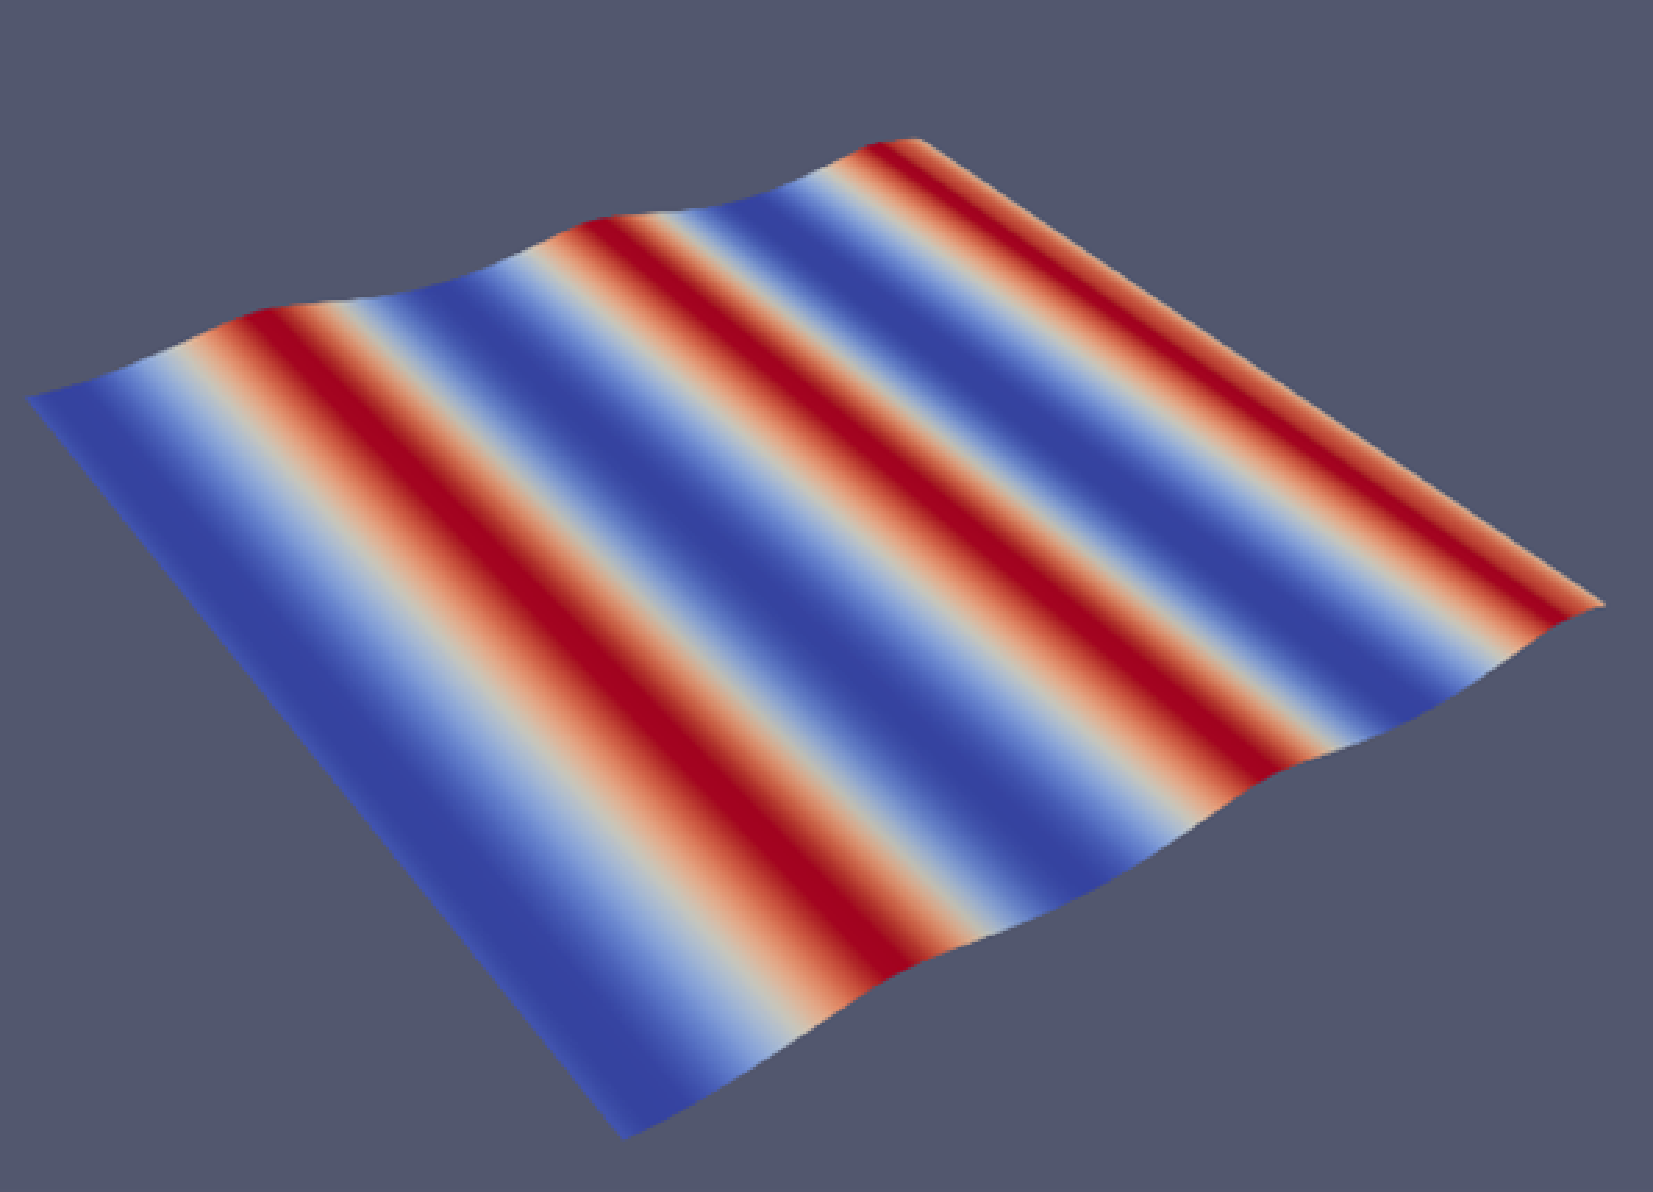
\includegraphics[width=0.8\linewidth]{FIGURE/wave_benchmark.pdf}}
\caption{\black{User Datagram Protocol (UDP)}}
\label{UDP}
\end{figure}

\begin{figure}[htb]
\centerline{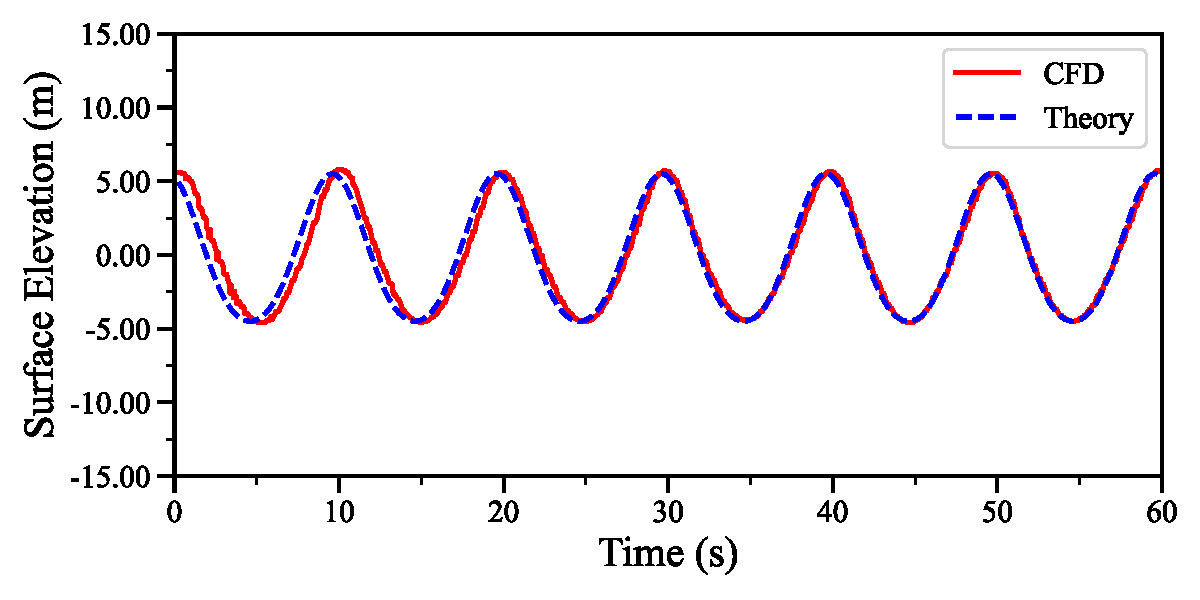
\includegraphics[width=0.8\linewidth]{FIGURE/wave_surface_vs_time.pdf}}
\caption{\black{User Datagram Protocol (UDP)}}
\label{UDP}
\end{figure}

\subsection{Wave generation}

This study employs two dynamic mesh techniques: morphing and overset mesh\citet{quallen2013cfd, tran2016fully}. Morphing mesh is applied to model the six-degree-of-freedom motion of the floating platform and tower, while the overset mesh approach is utilized to capture the rotational motion of the wind turbine. 
Morphing mesh allow continuous object motion by distorting the existing computational mesh without altering its topology, thereby avoiding remeshing and preserving both computational efficiency and numerical stability during platform motion. In contrast, the overset mesh technique enables relative motion between components by overlapping independently generated meshes which exchange information via interpolation. This method offers greater flexibility for handling large rotations and complex interactions.
While morphing mesh offers faster computation and easier implementation, they are generally unsuitable for continuous rotational motion. In contrast, overset meshes, though more computationally expensive and requiring predefined background and component meshes, provide greater versatility and are better suited for simulations involving complex or multi-degree-of-freedom motion. Therefore, this study adopts a hybrid approach that combines both methods to leverage their respective advantages.

This study employed two dynamic meshing techniques: morphing meshes and overset meshes\citet{quallen2013cfd, tran2016fully}, to capture the complex motions of floating offshore wind turbines (FOWTs). The morphing mesh method was primarily applied to simulate the six-degree-of-freedom motion of the floating platform and tower, while the overset mesh method was used to represent the continuous rotational motion of the wind turbine blades. The combination of these two approaches balances numerical stability with geometric flexibility, enabling a more comprehensive representation of fluid–structure interaction effects during turbine operation.

Mesh deformation achieves continuous structural motion by smoothly interpolating shape functions and adjusting node positions within the existing computational mesh, without altering its overall topology. This method avoids frequent remeshing and ensures computational efficiency and numerical stability during translational, heave, and small-amplitude sway motions. It is particularly effective for simulating low-frequency, large-scale platform dynamics, as it reduces numerical dissipation and interpolation errors. However, excessive mesh distortion may occur during prolonged or large-scale motion, leading to reduced accuracy or numerical instability. Consequently, this method is unsuitable for continuous, large-scale rotational motions.

The overset mesh technique, also referred to as the Chimera method, employs multiple independently generated mesh systems. A background mesh resolves the large-scale flow field, while local sub-meshes discretize complex moving components such as rotating blades and towers. Information exchange between meshes is achieved through interpolation, which allows natural treatment of relative motion. This technique offers high flexibility in handling large rotations, multi-degree-of-freedom coupling, and complex geometries, while avoiding mesh distortion. Its main limitation is higher computational cost, as it requires careful definition of overlap regions during preprocessing and stable interpolation throughout the calculation.

In summary, the morphing mesh method provides high efficiency and robustness for large-scale but low-frequency platform motions, whereas the overset mesh method offers greater accuracy and flexibility for continuous blade rotation, although with higher computational cost. To leverage the strengths of both approaches, this study adopted a hybrid strategy. Morphing meshes were used for platform and tower motions, while overset meshes were applied to the rotor. This complementary strategy enhances both accuracy and efficiency, providing a robust technical foundation for high-fidelity aerodynamic, hydrodynamic, and structural coupled simulations of FOWTs.

\subsection{Mooring system}

In this study, the mooring forces were calculated using Moody, a numerical tool specifically developed for cable dynamics analysis with primary applications in mooring system research within offshore engineering. Moody can be employed as a standalone solver or coupled with external computational fluid dynamics (CFD) software, such as OpenFOAM, through an application programming interface (API), thereby enabling advanced fluid–structure interaction simulations. The solver is based on the discontinuous Galerkin finite element method, incorporating high-order Legendre polynomial expansions and a Lax–Friedrich-type Riemann solver. This formulation provides high accuracy and stability when addressing complex problems such as nonlinear tension response, impact loading, and seabed contact.

Moody adopts a flexible input file structure that supports the definition of cable material models, boundary conditions, rigid body objects, and foundation models. It accommodates multiple execution modes, including command-line operation, batch processing, and MATLAB interfaces, and provides post-processing utilities for analyzing cable tension, displacement, and dynamic response. The code is compact and independent of external libraries, ensuring portability across Linux, macOS, and Windows platforms.

Owing to these capabilities, Moody has been widely applied in the dynamic analysis of marine structures, including floating offshore wind turbines and wave energy conversion devices. It thus provides a reliable and practical tool that bridges fundamental research and engineering applications in offshore system dynamics.

\section{Validation}  

\subsection{Model description}  

The IEA Wind 15-Megawatt Offshore Reference Wind Turbine\citet{gaertner2020definition} and the UMaine VolturnUS-S Reference Platform\citet{allen2020definition} are adopted as the baseline models in this study. The key parameters of both models are summarized in Table \ref{tab:WT_parameters}. The verification process is divided into two parts: (1) the aerodynamic performance of the wind turbine, and (2) the hydrodynamic response of the floating platform.

\begin{table}[t]
    \centering
    \caption{Parameters of wind turbine and floating platform}
    \label{tab:WT_parameters}
    \begin{tabular}{cccccc}
    % \toprule\hline
  \hline\hline
        \textbf{Type} & \textbf{Value}   \\ \midrule
         Rated power & 15 MW   \\ 
         Rated wind speed & 10.59 m/s     \\
         Rotor diameter & 240 m     \\
         Maximum rotor speed & 7.56 rpm   \\ 
         Precone angle & $4^\circ$  \\
         Shaft tilt angle & $6^\circ$      \\
         Platform type & Semisubmersible    \\ 
         Total system mass & 20093 t   \\
         Water depth & 200 m     \\
    \hline\hline
    % \bottomrule
    \end{tabular}
\end{table}

% 注释：可以再加点图
\subsection{Aerodynamics}

To verify the aerodynamic performance of the framework, simulation results for the IEA Wind 15 MW offshore reference turbine at rated wind speed are compared with OpenFAST under identical inflow conditions. Overset mesh is employed in this section to accommodate rotational motion of rotor. As illustrated in Figure \ref{Rotor}, the left shows the oversetpatch (Interpolation surface), while the right displays rotor geometry. The blade surface is discretized using a boundary layer mesh consisting of 8 layers, with a growth rate of 1.2 and a first-layer thickness of 0.005 m, ensuring adequate resolution of near-wall flow features. 

\begin{figure}[htb]
\centerline{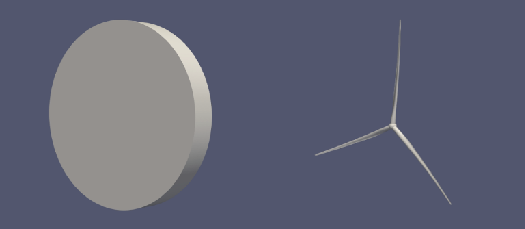
\includegraphics[width=0.8\linewidth]{FIGURE/Rotor.pdf}}
\caption{Oversetpatch and Rotor}
\label{Rotor}
\end{figure}

This section presents a numerical simulation of rotor thrust and torque under rated rotor speed and inflow conditions. The spanwise distributions of normal and tangential blade forces are extracted and compared with OpenFAST results.
Table 3 presents the comparison of rotor thrust and torque between the present simulation and OpenFAST results, showing good overall agreement.


\subsection{Hydrodynamics}

This section evaluates the hydrodynamic performance of the University of Maine VolturnUS-S reference platform through free-decay tests. Such tests are widely used to identify a platform’s natural frequencies and damping characteristics, and they provide an effective means of verifying the accuracy of numerical models. In this study, the response characteristics of both the full-scale platform and a scaled model were examined. The full-scale hydrodynamic results were compared with OpenFAST simulations to validate the numerical predictions, while the scaled model behavior was cross-checked against experimental data from the University of Plymouth. This two-level comparison established consistency between experimental and numerical results and further enhanced the reliability of the simulation framework.

For the representation of mooring forces and platform motion, the open-source tool Moody and deformable meshing techniques were employed, respectively, to ensure accurate modeling of mooring coupling and six-degree-of-freedom platform dynamics. Through multiple layers of validation, including numerical–experimental and full-scale–scaled comparisons, the analytical framework developed in this study was demonstrated to be robust, thereby providing a solid foundation for subsequent high-fidelity coupled simulations of floating wind turbines.

\subsubsection{Validation of the Full-scale Model}

The hydrodynamic performance of the full-scale IEA 15 MW was evaluated through free decay tests in three directions: surge, pitch, and heave.

Static Equilibrium Tests. As the initial step of the full-scale hydrodynamic validation, a static equilibrium test incorporating the mooring system was performed. After 60 seconds, the system stabilized at a center of mass (COM) position of (0.3, 0, −2.375), with a corresponding pitch angle of $-1.32^\circ$. The results closely matched OpenFAST, which reported a COM of (0.367, 0, −2.693) and a pitch angle of $-1.484^\circ$.

Moored decay tests. For the free decay tests, the equilibrium position obtained from the preceding static analysis was used as the initial condition. Prescribed offsets in surge, pitch, and heave were then applied, as detailed in Table 2.

\begin{table}[t]
    \centering
    \caption{Initial offsets for free-decay tests}
    \label{tab:decay_cases}
    \begin{tabular}{lccc}
    \hline\hline
        \textbf{Case} & \textbf{Offset in surge} & \textbf{Offset in pitch} & \textbf{Offset in heave} \\ \hline
        Surge decay  & $30^\circ$ & 0 & 0 \\
        Pitch decay  & 0 & $11^\circ$ & 0 \\
        Heave decay  & 0 & 0 & 5 \\
    \hline\hline
    \end{tabular}
\end{table}
\textbf{Surge decay.} Figure \ref{Full surge} compares the numerically simulated surge motion and mooring tensions with the corresponding FAST results.

\begin{figure}
    \centering

    \begin{subfigure}{0.9\linewidth} % 第一个子图
        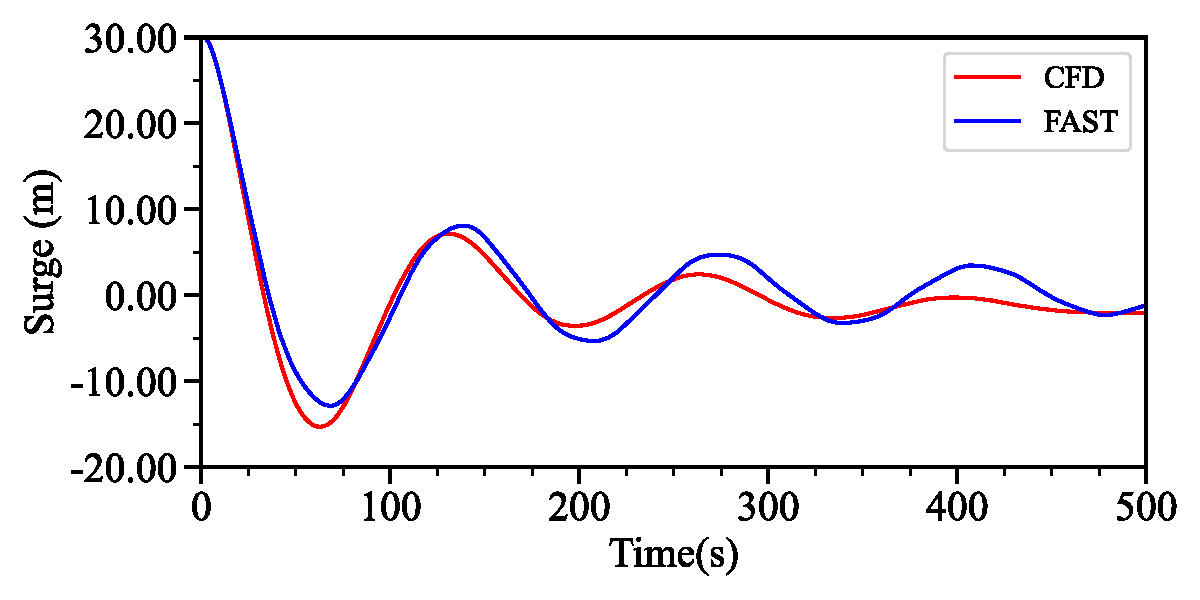
\includegraphics[width=\linewidth]{FIGURE/Full-Hydrodynamics/Surge.pdf}
        \caption{\black{Training curve of reward}}
        \label{reward_3}
    \end{subfigure}
    \begin{subfigure}{0.9\linewidth} % 第一个子图
        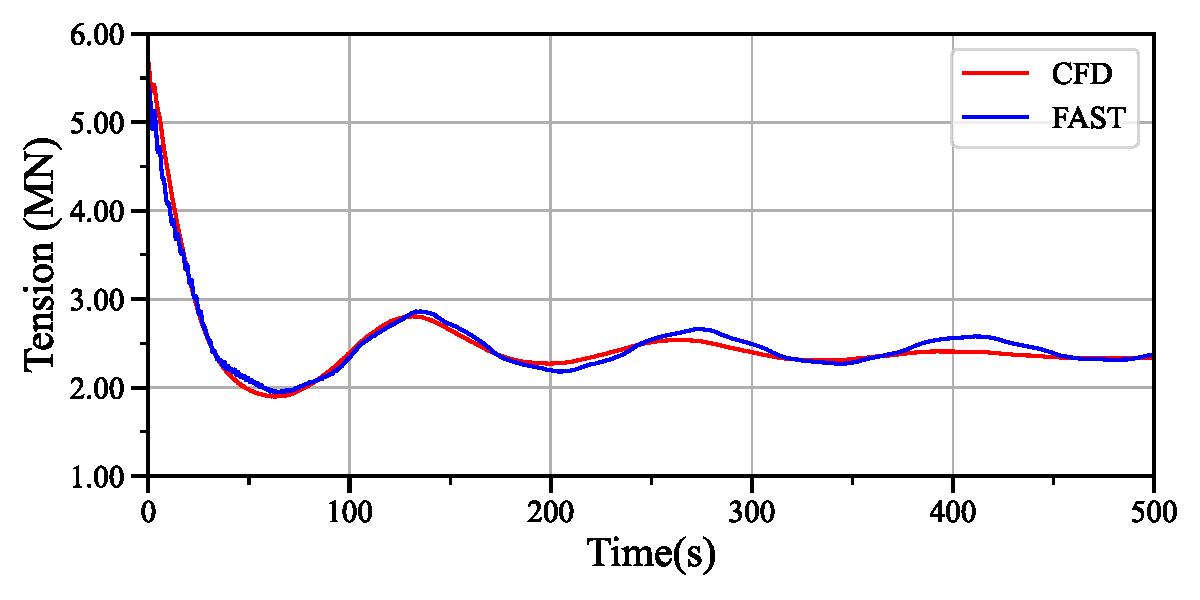
\includegraphics[width=\linewidth]{FIGURE/Full-Hydrodynamics/Surge_Tension_1.pdf}
        \caption{\black{Training curve of Mean $C_d$}}
        \label{Cd_3}
    \end{subfigure}
    % \hspace{0.5\linewidth}
    \begin{subfigure}{0.9\linewidth} % 第二个子图
        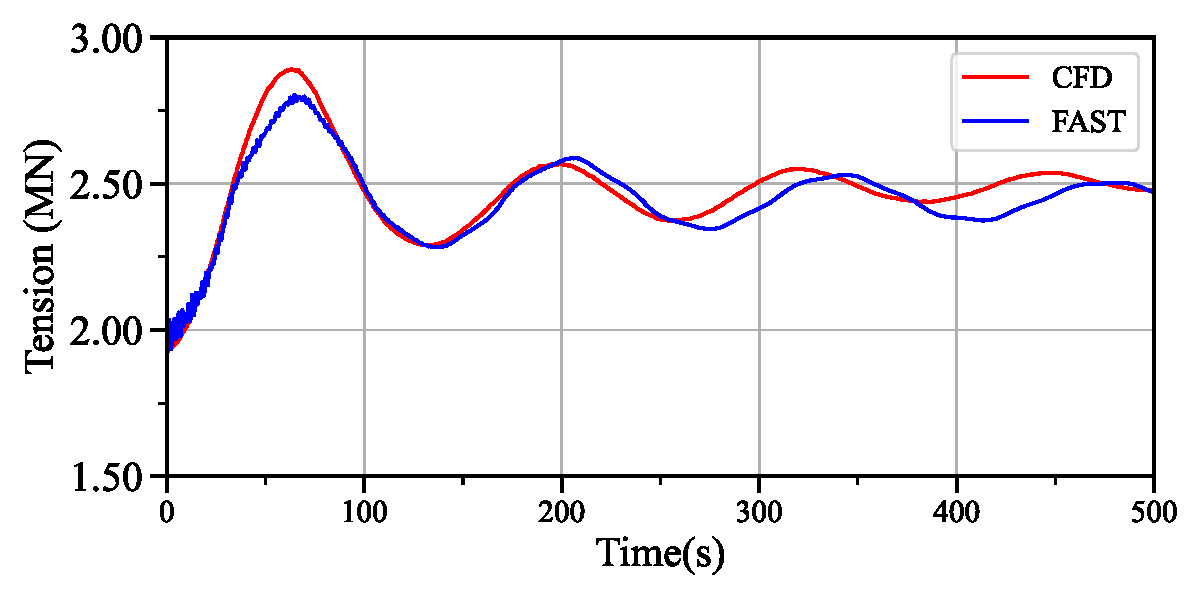
\includegraphics[width=\linewidth]{FIGURE/Full-Hydrodynamics/Surge_Tension_2.pdf}
        \caption{\black{Training curve of Std $C_l$}}
        \label{Cl_3}
    \end{subfigure}
    
    \caption{Surge decay test of full-scale model. Surge motion, fore and aft mooring tension.}
    \label{Full surge}
\end{figure}

\textbf{Pitch decay.} Figure \ref{Full pitch} compares the numerically simulated pitch motion and mooring tensions with the corresponding FAST results.

\begin{figure}
    \centering

    \begin{subfigure}{0.9\linewidth} % 第一个子图
        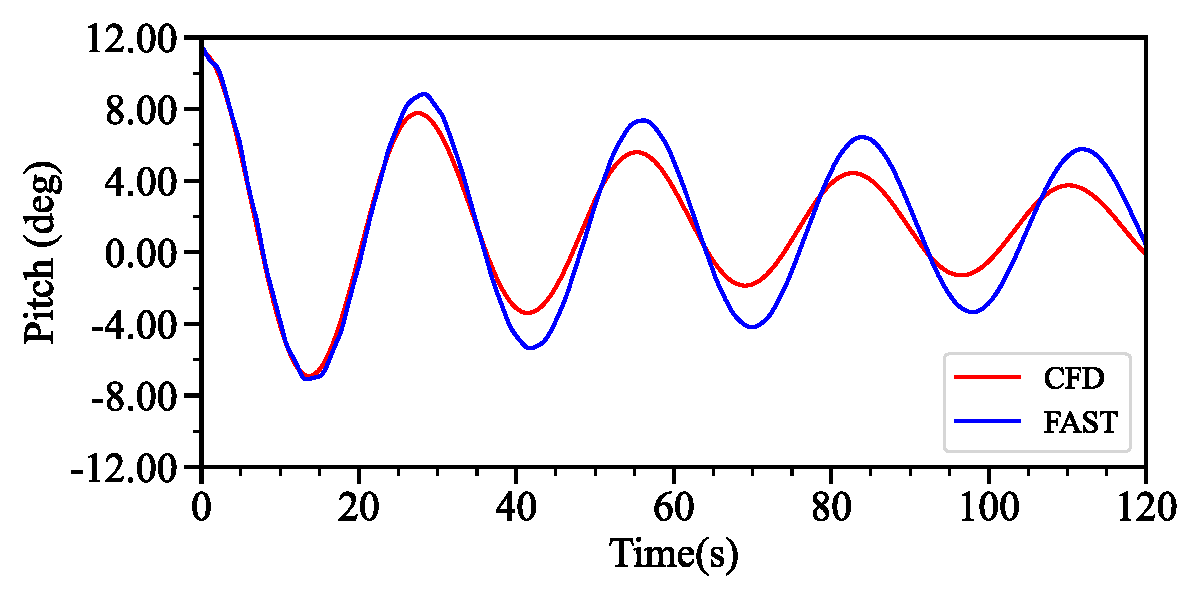
\includegraphics[width=\linewidth]{FIGURE/Full-Hydrodynamics/Pitch.pdf}
        \caption{\black{Training curve of reward}}
        \label{reward_3}
    \end{subfigure}
    \begin{subfigure}{0.9\linewidth} % 第一个子图
        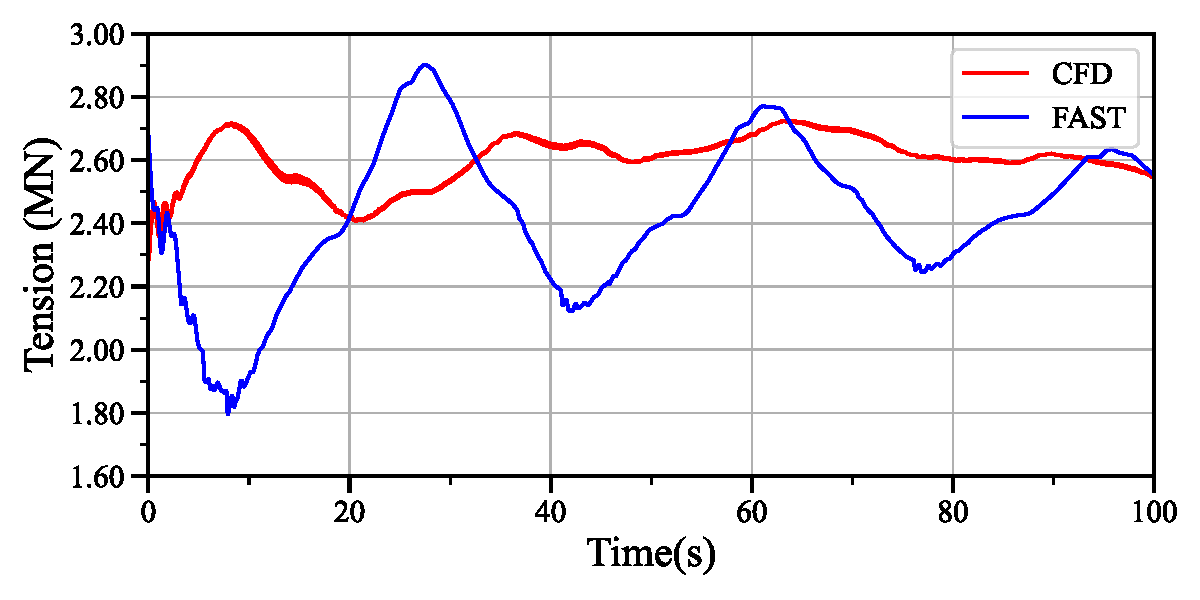
\includegraphics[width=\linewidth]{FIGURE/Full-Hydrodynamics/Pitch_Tension_1.pdf}
        \caption{\black{Training curve of Mean $C_d$}}
        \label{Cd_3}
    \end{subfigure}
    % \hspace{0.5\linewidth}
    \begin{subfigure}{0.9\linewidth} % 第二个子图
        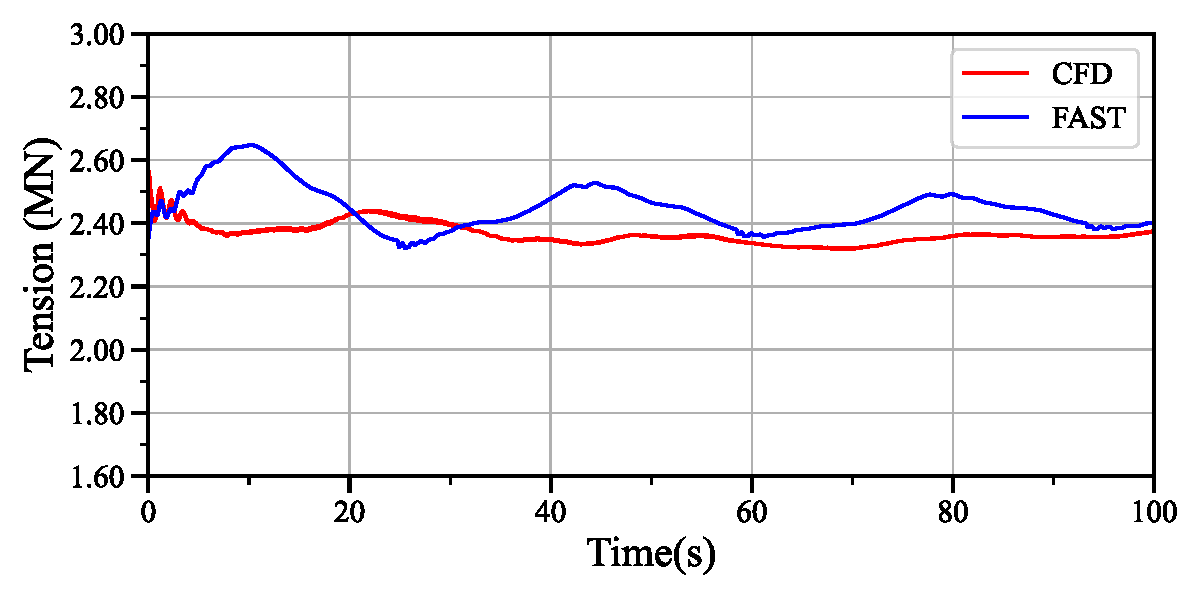
\includegraphics[width=\linewidth]{FIGURE/Full-Hydrodynamics/Pitch_Tension_2.pdf}
        \caption{\black{Training curve of Std $C_l$}}
        \label{Cl_3}
    \end{subfigure}
    
    \caption{Pitch decay test of full-scale model. Pitch motion, fore and aft mooring tension.}
    \label{Full pitch}
\end{figure}

\textbf{Heave decay.} Figure \ref{Full heave} compares the numerically simulated pitch motion and mooring tensions with the corresponding FAST results.

\begin{figure}
    \centering

    \begin{subfigure}{0.9\linewidth} % 第一个子图
        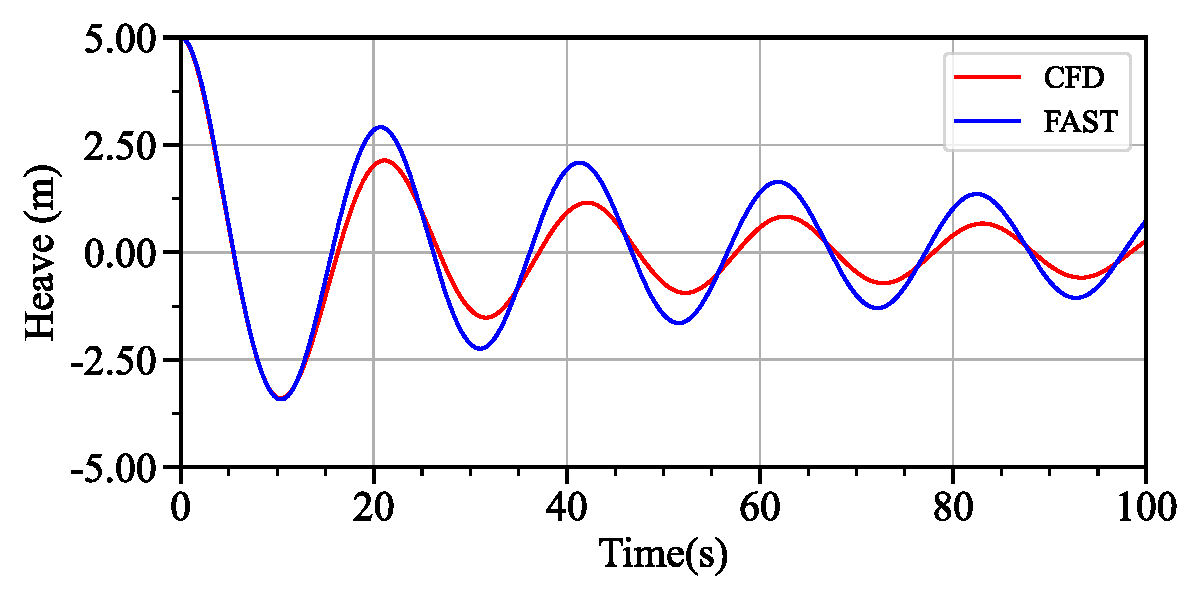
\includegraphics[width=\linewidth]{FIGURE/Full-Hydrodynamics/Heave.pdf}
        \caption{\black{Training curve of reward}}
        \label{reward_3}
    \end{subfigure}
    \begin{subfigure}{0.9\linewidth} % 第一个子图
        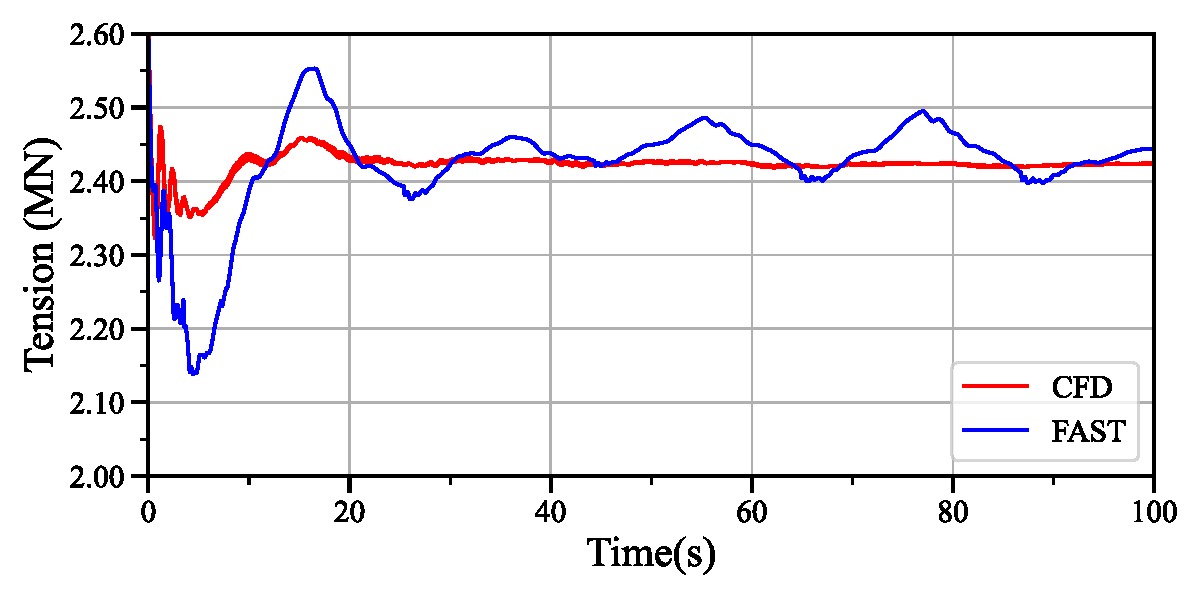
\includegraphics[width=\linewidth]{FIGURE/Full-Hydrodynamics/Heave_Tension_1.pdf}
        \caption{\black{Training curve of Mean $C_d$}}
        \label{Cd_3}
    \end{subfigure}
    % \hspace{0.5\linewidth}
    \begin{subfigure}{0.9\linewidth} % 第二个子图
        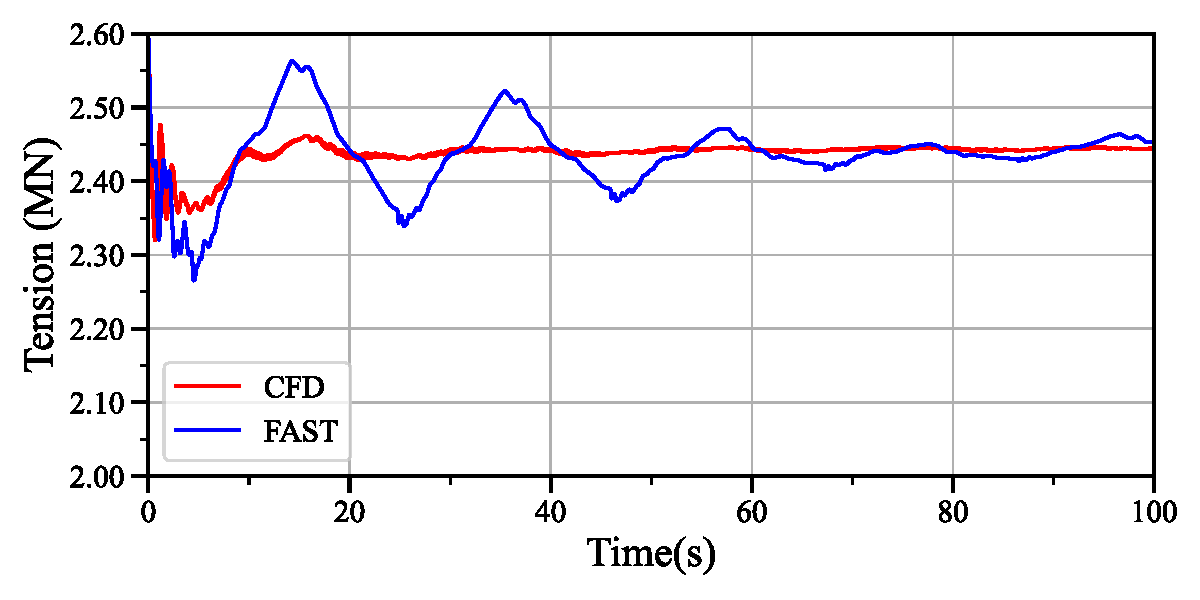
\includegraphics[width=\linewidth]{FIGURE/Full-Hydrodynamics/Heave_Tension_2.pdf}
        \caption{\black{Training curve of Std $C_l$}}
        \label{Cl_3}
    \end{subfigure}
    
    \caption{Heave decay test of full-scale model. Heave motion, fore and aft mooring tension.}
    \label{Full heave}
\end{figure}

Table 3 provides a comparison of the natural frequencies and damping ratios obtained from the free decay tests and corresponding numerical simulations for the three degrees of freedom.

\begin{table}[t]
    \centering
    \caption{Natural frequency and damping ratio for different decay tests of full-scale model.}
    \label{tab:decay_results}
    \begin{tabular}{llcc}
    \hline\hline
        \textbf{Case} & \textbf{Method} & \textbf{Frequency (Hz)} & \textbf{Damping ratio} \\ \hline
        Surge  & EXP & 0.007 & 0.0012 \\
        Surge  & CFD & 0.008 & 0.0015 \\
        Pitch  & EXP & 0.035 & 0.0014 \\
        Pitch  & CFD & 0.037 & 0.0024 \\
        Heave  & EXP & 0.048 & 0.0035 \\
        Heave  & CFD & 0.048 & 0.0056 \\
    \hline\hline
    \end{tabular}
\end{table}

\subsubsection{Validation of the scaled Model}

The experimental validation employs a 1:70 scaled model to assess the hydrodynamic response of the floating platform in three degrees of freedom: surge, pitch, and heave.

Static Equilibrium Tests. As the first step in the hydrodynamic verification, a static equilibrium test incorporating the mooring system was conducted. After 60 seconds, the simulated center of mass (COM) of the FOWT stabilized at (−0.011, 0, −0.0214), with a pitch angle of $-1.35^\circ$. The results closely matched the experimental measurements, which reported a COM of (−0.02038, 0, −0.02386) and a pitch angle of $-1.502^\circ$.

Moored decay tests. For the free decay tests, the initial condition was set based on the static equilibrium position obtained in the previous section. Offsets were then applied in the surge, pitch, and heave directions, as summarized in Table \ref{tab:decay_offset_scaled}.

\begin{table}[t]
    \centering
    \caption{Decay tests offset of scaled model.}
    \label{tab:decay_offset_scaled}
    \begin{tabular}{lccc}
    \hline\hline
        \textbf{Case} & \textbf{Offset in surge (m)} & \textbf{Offset in pitch (deg)} & \textbf{Offset in heave (m)} \\ \hline
        Surge decay  &  0.3825  &  -0.7657  &  -0.0017 \\
        Pitch decay  & -0.0031  &  -9.7980  &  -0.0277 \\
        Heave decay  & -0.0149  &   0.4719  &  -0.1472 \\
    \hline\hline
    \end{tabular}
\end{table}

\textbf{Surge decay.} Figure \ref{scaled surge} compares the numerically simulated surge motion and mooring tensions with the corresponding experimental results.
\begin{figure}
    \centering

    \begin{subfigure}{0.9\linewidth} % 第一个子图
        
\includegraphics[width=\linewidth]{FIGURE/scaled-Hydrodynamics/Surge.pdf}
        \caption{\black{Training curve of reward}}
        \label{reward_3}
    \end{subfigure}
    \begin{subfigure}{0.9\linewidth} % 第一个子图
        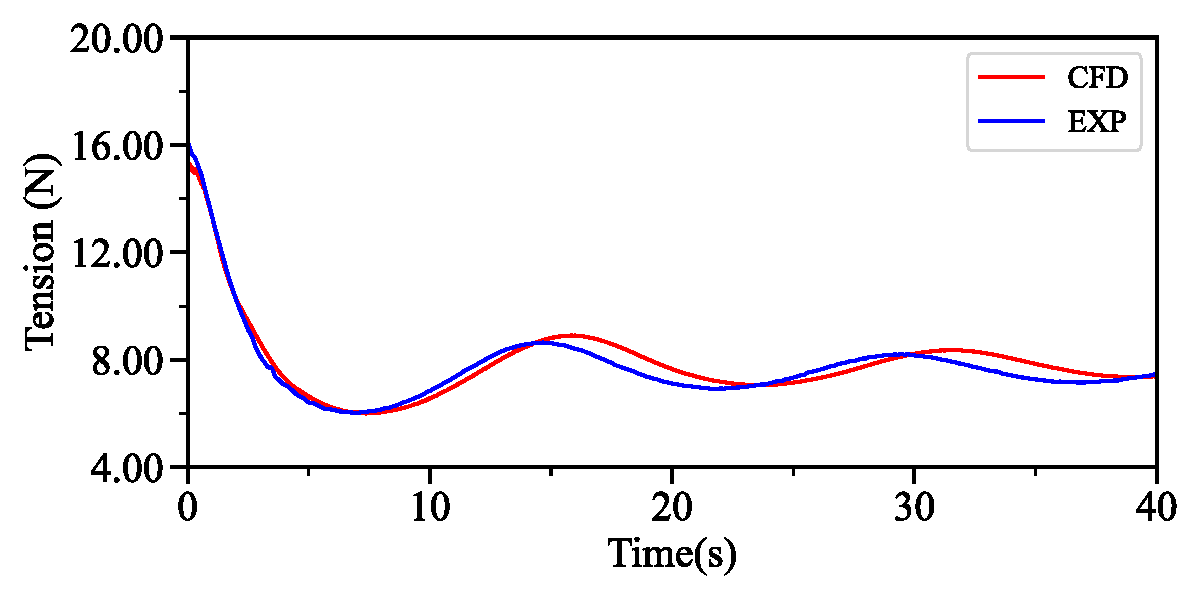
\includegraphics[width=\linewidth]{FIGURE/scaled-Hydrodynamics/scaled_surge_cable1.pdf}
        \caption{\black{Training curve of Mean $C_d$}}
        \label{Cd_3}
    \end{subfigure}
    % \hspace{0.5\linewidth}
    \begin{subfigure}{0.9\linewidth} % 第二个子图
        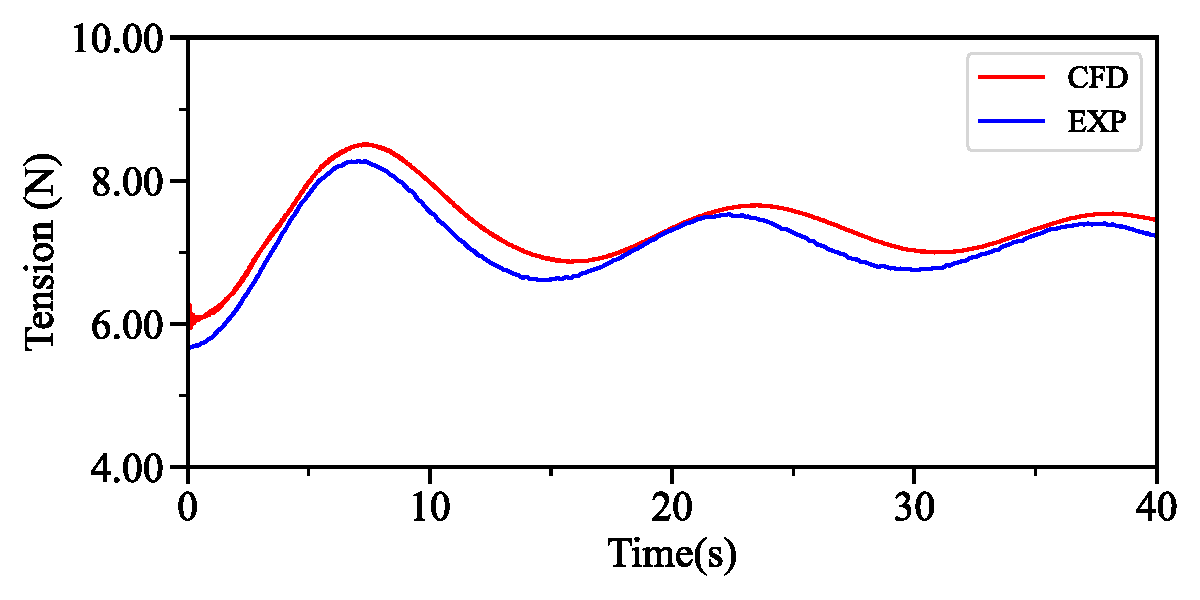
\includegraphics[width=\linewidth]{FIGURE/scaled-Hydrodynamics/scaled_surge_cable2.pdf}
        \caption{\black{Training curve of Std $C_l$}}
        \label{Cl_3}
    \end{subfigure}
    
    \caption{Heave decay test of full-scale model. Heave motion, fore and aft mooring tension.}
    \label{scaled surge}
\end{figure}

\textbf{Pitch decay.} Figure \ref{scaled pitch} compares the numerically simulated pitch motion and mooring tensions with the corresponding experimental results.
\begin{figure}
    \centering

    \begin{subfigure}{0.9\linewidth} % 第一个子图
        
\includegraphics[width=\linewidth]{FIGURE/scaled-Hydrodynamics/Pitch.pdf}
        \caption{\black{Training curve of reward}}
        \label{reward_3}
    \end{subfigure}
    \begin{subfigure}{0.9\linewidth} % 第一个子图
        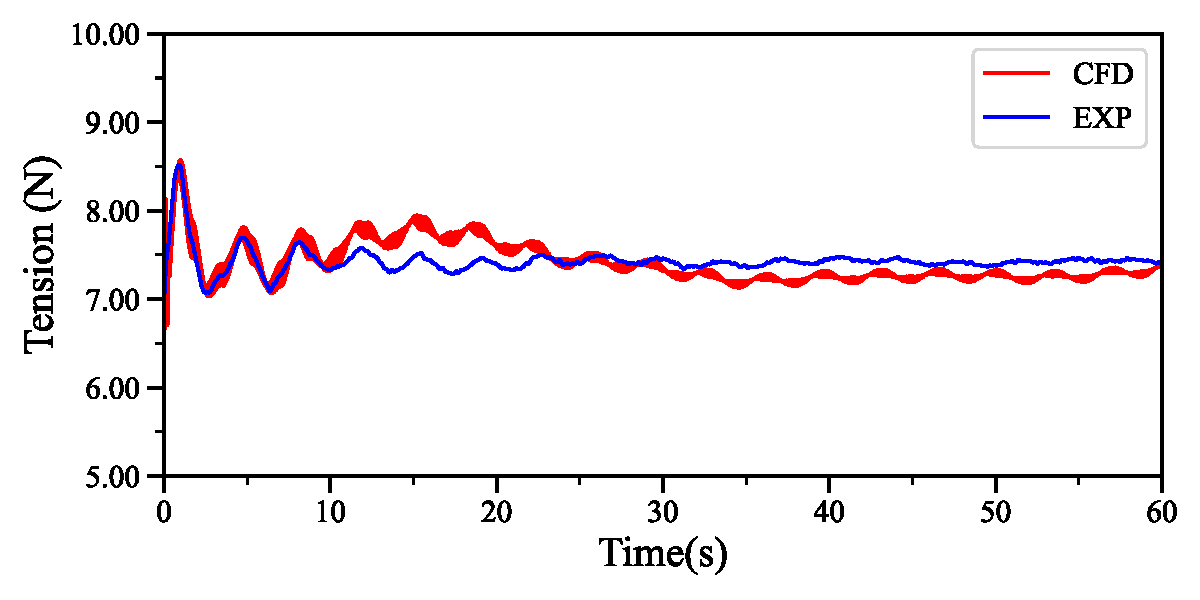
\includegraphics[width=\linewidth]{FIGURE/scaled-Hydrodynamics/scaled_pitch_cable1.pdf}
        \caption{\black{Training curve of Mean $C_d$}}
        \label{Cd_3}
    \end{subfigure}
    % \hspace{0.5\linewidth}
    \begin{subfigure}{0.9\linewidth} % 第二个子图
        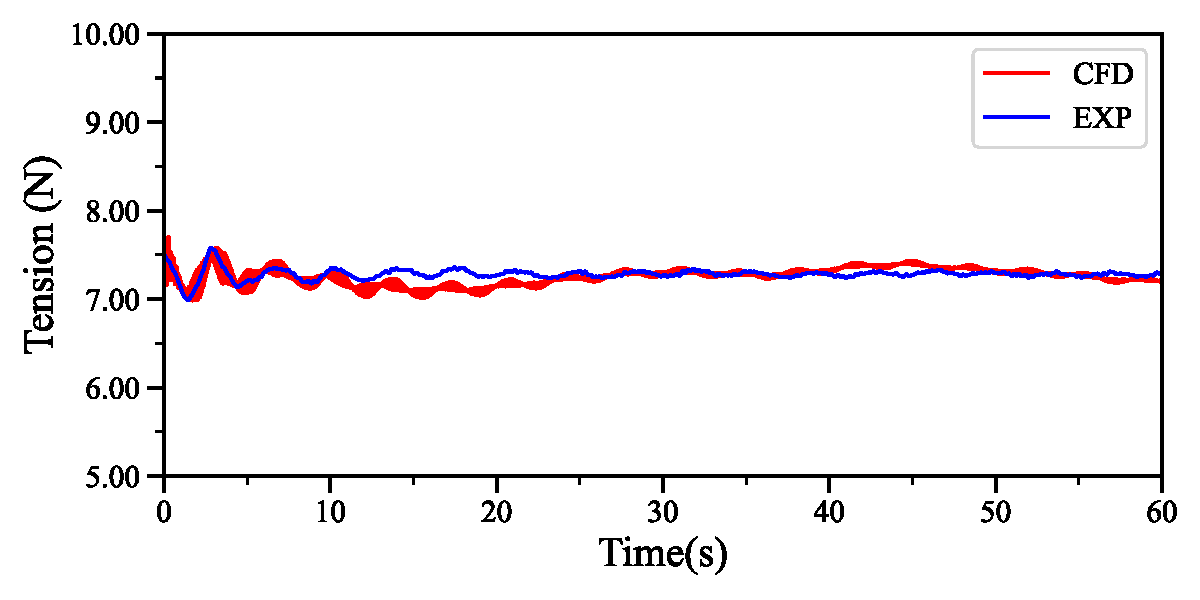
\includegraphics[width=\linewidth]{FIGURE/scaled-Hydrodynamics/scaled_pitch_cable2.pdf}
        \caption{\black{Training curve of Std $C_l$}}
        \label{Cl_3}
    \end{subfigure}
    
    \caption{Heave decay test of full-scale model. Heave motion, fore and aft mooring tension.}
    \label{scaled pitch}
\end{figure}
\textbf{Heave decay.} Figure \ref{scaled heave} compares the numerically simulated heave motion and mooring tensions with the corresponding experimental results.
\begin{figure}
    \centering

    \begin{subfigure}{0.9\linewidth} % 第一个子图
        
\includegraphics[width=\linewidth]{FIGURE/scaled-Hydrodynamics/Heave.pdf}
        \caption{\black{Training curve of reward}}
        \label{reward_3}
    \end{subfigure}
    \begin{subfigure}{0.9\linewidth} % 第一个子图
        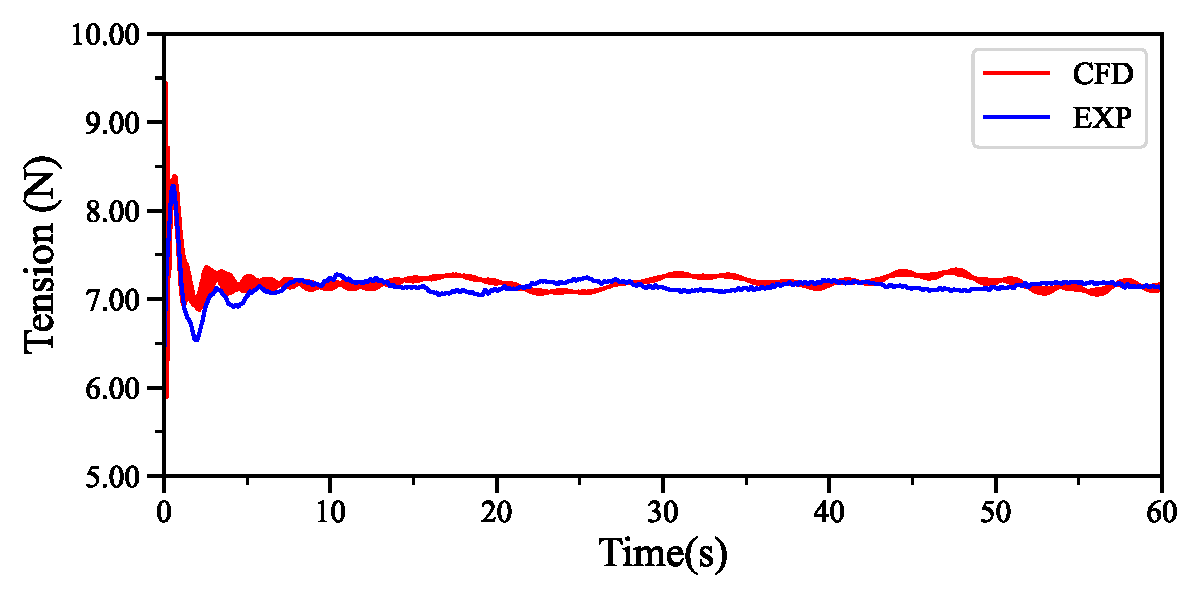
\includegraphics[width=\linewidth]{FIGURE/scaled-Hydrodynamics/scaled_heave_cable1.pdf}
        \caption{\black{Training curve of Mean $C_d$}}
        \label{Cd_3}
    \end{subfigure}
    % \hspace{0.5\linewidth}
    \begin{subfigure}{0.9\linewidth} % 第二个子图
        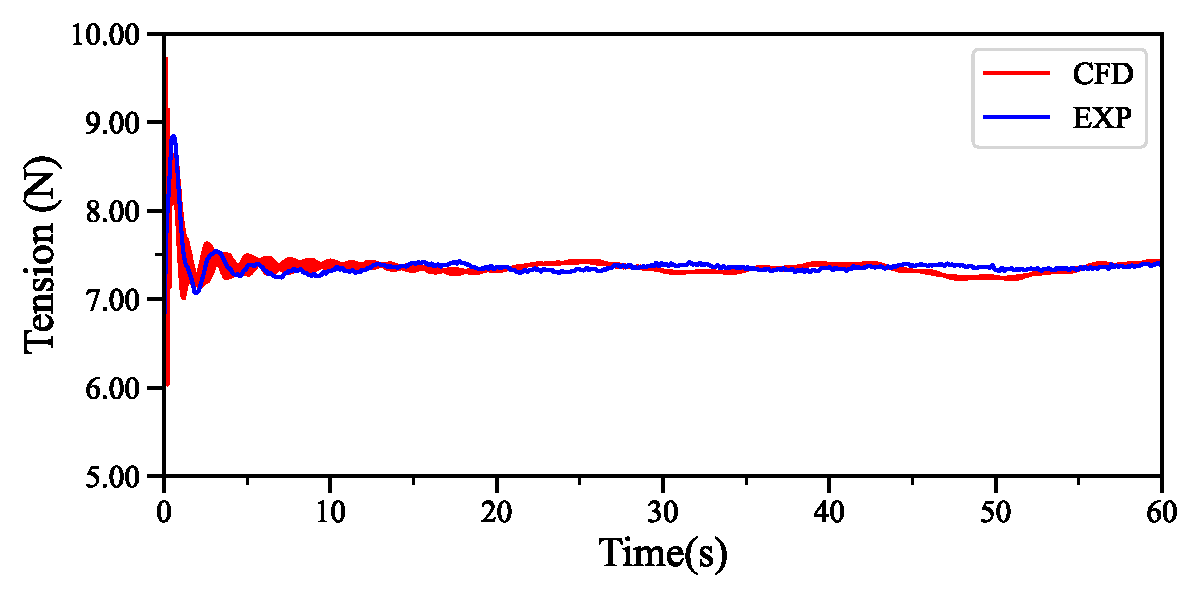
\includegraphics[width=\linewidth]{FIGURE/scaled-Hydrodynamics/scaled_heave_cable2.pdf}
        \caption{\black{Training curve of Std $C_l$}}
        \label{Cl_3}
    \end{subfigure}
    
    \caption{Heave decay test of full-scale model. Heave motion, fore and aft mooring tension.}
    \label{scaled heave}
\end{figure}

Table \ref{tab:decay_results_scaled} presents a comparison of the natural frequencies and damping ratios obtained from the free decay tests and the corresponding numerical simulations for all three degrees of freedom.

\begin{table}[t]
  \centering
  \caption{Natural frequency and damping ratio for different decay tests of scaled model.}
  \label{tab:decay_results_scaled}
  \begin{tabular}{llcc}
    \hline\hline
    \textbf{Case} & \textbf{Method} & \textbf{Frequency (Hz)} & \textbf{Damping ratio} \\ \hline
    Surge & EXP & 0.0639 & 0.0090 \\
    Surge & CFD & 0.0650 & 0.0093 \\
    Pitch & EXP & 0.2730 & 0.0124 \\
    Pitch & CFD & 0.2900 & 0.0110 \\
    Heave & EXP & 0.4000 & 0.0333 \\
    Heave & CFD & 0.4000 & 0.0374 \\
    \hline\hline
  \end{tabular}
\end{table}

The results indicate that the combination of morphing mesh approach and the mooring system effectively captures the hydrodynamic behavior of FOWT. Notably, the damping ratios obtained from the CFD-based full-scale simulations are significantly higher than those predicted by OpenFAST, which can be attributed to the ability of CFD to more accurately account for viscous effects.

\subsection{Deep reinforcement learning setup}

This study employs the SAC algorithm \cite{haarnoja2018soft}, which is one of the most widely used DRL algorithms. Unlike the on-policy method of PPO \cite{schulman2017proximal}, SAC demonstrates higher data utilization. Additionally, compared to TD3 \cite{fujimoto2018addressing}, SAC requires less parameter tuning.

SAC uses off-policy learning, allowing for data reuse during training, thereby achieving high data utilization. This means that collected experience can be effectively used multiple times, improving learning efficiency. Furthermore, off-policy learning enables the use of two different strategies during the iteration process, allowing flexible adjustment of the exploration probability to achieve effective exploration and exploitation. By exploring various actions, the algorithm can better understand and optimize the strategy.

The algorithm aims to optimize the policy and continuously update its parameters to maximize the objective function, which is described in Equation \ref{con:rewardinDRL},

\begin{equation}
J^{*}(\pi)= \sum_{t} \mathbb{E}_{\left(s_{t}, a_{t}\right) \sim \rho_{\pi}} [\underbrace{R\left(s_{t}, a_{t}\right)}_{\text {reward}}+\alpha\underbrace{\mathcal{H}\left(\pi\left(\cdot \mid s_{t}\right)\right)}_{\text {entropy }}]
\label{con:rewardinDRL}
\end{equation}
where $\alpha$ represents the entropy coefficient, and $\mathcal{H}$ represents the entropy of the policy, which affects the randomness of the policy. The variables $(s, a, r, s')$ are derived from a Markov decision process, where the state space $S$ and the action space $A$ are continuous. $R(s_t, a_t)$ represents the reward associated with the current state-action pair, while $\mathbb{E}$ represents the mathematical expectation. Additionally, $\rho_\pi$ denotes the state and state-action marginals of the trajectory distribution induced by policy $\pi(a_t|s_t)$.

In summary, SAC, as an off-policy algorithm, offers advantages such as high data utilization, effective exploration, and the ability to utilize diverse data sources, making it well-suited for this experiment. Furthermore, in DRL tasks, the reward function is crucial because it guides the agent in learning the desired behavior. The reward function measures the effectiveness of the current strategy by providing positive reward for actions that are close to the goal and negative reward for actions that deviate from the goal. It guides the learning process of the agent, enabling it to maximize cumulative reward and learn the optimal behavior over time.

In this study, DRL training not only considered the suppression of drag and lift coefficients but also accounted for the energy consumption caused by blowing. Therefore, the reward function was set as the following equation \ref{multiple:rewardfunction}:

\begin{equation}
\begin{array}{l}
{{Reward} =  {\left| {{C_d}} \right|_0} - {\left| {{C_d}} \right|_T} + {\left\langle {{C_l}} \right\rangle _0} - {\left\langle {{C_l}} \right\rangle _T} - {\tilde a^{5 \times \tilde v}}}\\
\\
\tilde a = a/35,\ \tilde v = v/10
\end{array}
\label{multiple:rewardfunction}
\end{equation}
where $\tilde a$ and $\tilde v$  is normalized action and wind velocity, $a$ is flow rate for each hole, $v$ is incoming wind velocity, $\tilde a \  and \  \tilde v \in [0,1]$. $\left| \bullet \right|$ and $\left\langle \bullet \right\rangle $ represents mean and standard deviation value within the duration of pressure scanner. Subscript $0$ means no control, and subscript $T$ means step $T$ with DRL control. In this study, since it is a two-dimensional square cylinder model, the initial drag coefficient is ${\left| {{C_d}} \right|_0} = 2.1$ and the initial lift coefficient is ${\left\langle {{C_l}} \right\rangle _0} = 1.1$.

% Training setup
For the experimental setup, we used the SAC algorithm from the Stable Baselines3 library \cite{stable-baselines3}. SAC employed fully connected actor and critic neural networks, each consisting of two hidden layers with 256 neurons in each layer. Since the only environmental change factor in this study was the incoming wind velocity, the normalized incoming wind velocity ($\tilde{v}$) was used as the sole state, with the normalized blowing flow rate ($\tilde{a}$) as the action , as shown in FIG. \ref{DNN}.


\subsection{Usage of the DRLinWT platform}

In this example, the controller and sensor were the flow controller and pressure scanner respectively. The function of the flow controller was to adjust the blowing flow rate to achieve the actions dictated by the DRL algorithm, while the pressure scanner measured the wind pressure on the surface of the model. Based on these measurements, mean $C_d$  and std $C_l$ of the model were calculated, which were then used to determine the reward for the DRL algorithm.

The communication protocols used by the flow controller and pressure scanner were Modbus RTU and UDP. A universal adapter was employed to use the corresponding the appropriate communication protocol and configure the relevant parameters. The Adapter.W function was used to send commands to adjust the flow rate of the flow controller and send a "start scanning" command to the pressure scanner. The Adapter.R function was then used to obtain feedback or measurement data, as illustrated in FIG. \ref{EXP1}.

\subsection{Results}

In case 1, the learning rate was maintained at 0.001, and batch size gradually increased to 128, 256, and 512 with the number of training steps, hyperparameters were shown in Table \ref{hyperparameter in E1}. The reward curve during the training process was shown in FIG. \ref{reward-1}. The reward initially fluctuated within a large range but stabilized between $0.8 \sim 1.2$ after 400 steps, exhibiting a periodic fluctuation pattern. The final stable periodicity was due to the convergence of the control strategy. As the system adapted to the periodic changes in wind velocity, it developed a corresponding periodic response strategy. This resulted in a control effect and reward that also exhibited periodic behavior. Additionally, the change curves of mean $C_d$ and std $C_l$ during the training process were observed. After 400 steps, both $C_d$ and $C_l$ stabilized at low values, as shown in FIG. \ref{Cd-1} and FIG. \ref{Cl-1}.

\begin{table}[t]
    \centering
    \caption{Hyperparameters of training in case 1}
    \label{hyperparameter in E1}
    \setlength{\tabcolsep}{5mm}{
    \begin{tabular}{cccccc}
    % \toprule\hline
  \hline\hline
        \textbf{Hyperparameter} && \textbf{Value} \\ \midrule
         Neural network && [256, 256] &       \\ 
         Learning rate && 0.001 &        \\
         Gradient steps && 10 &     \\
         Batch size && 128, 256, 512  &      \\
    \hline\hline
    % \bottomrule
    \end{tabular} }
\end{table}

\begin{figure}
    \centering

    \begin{subfigure}{0.9\linewidth} % 第一个子图
        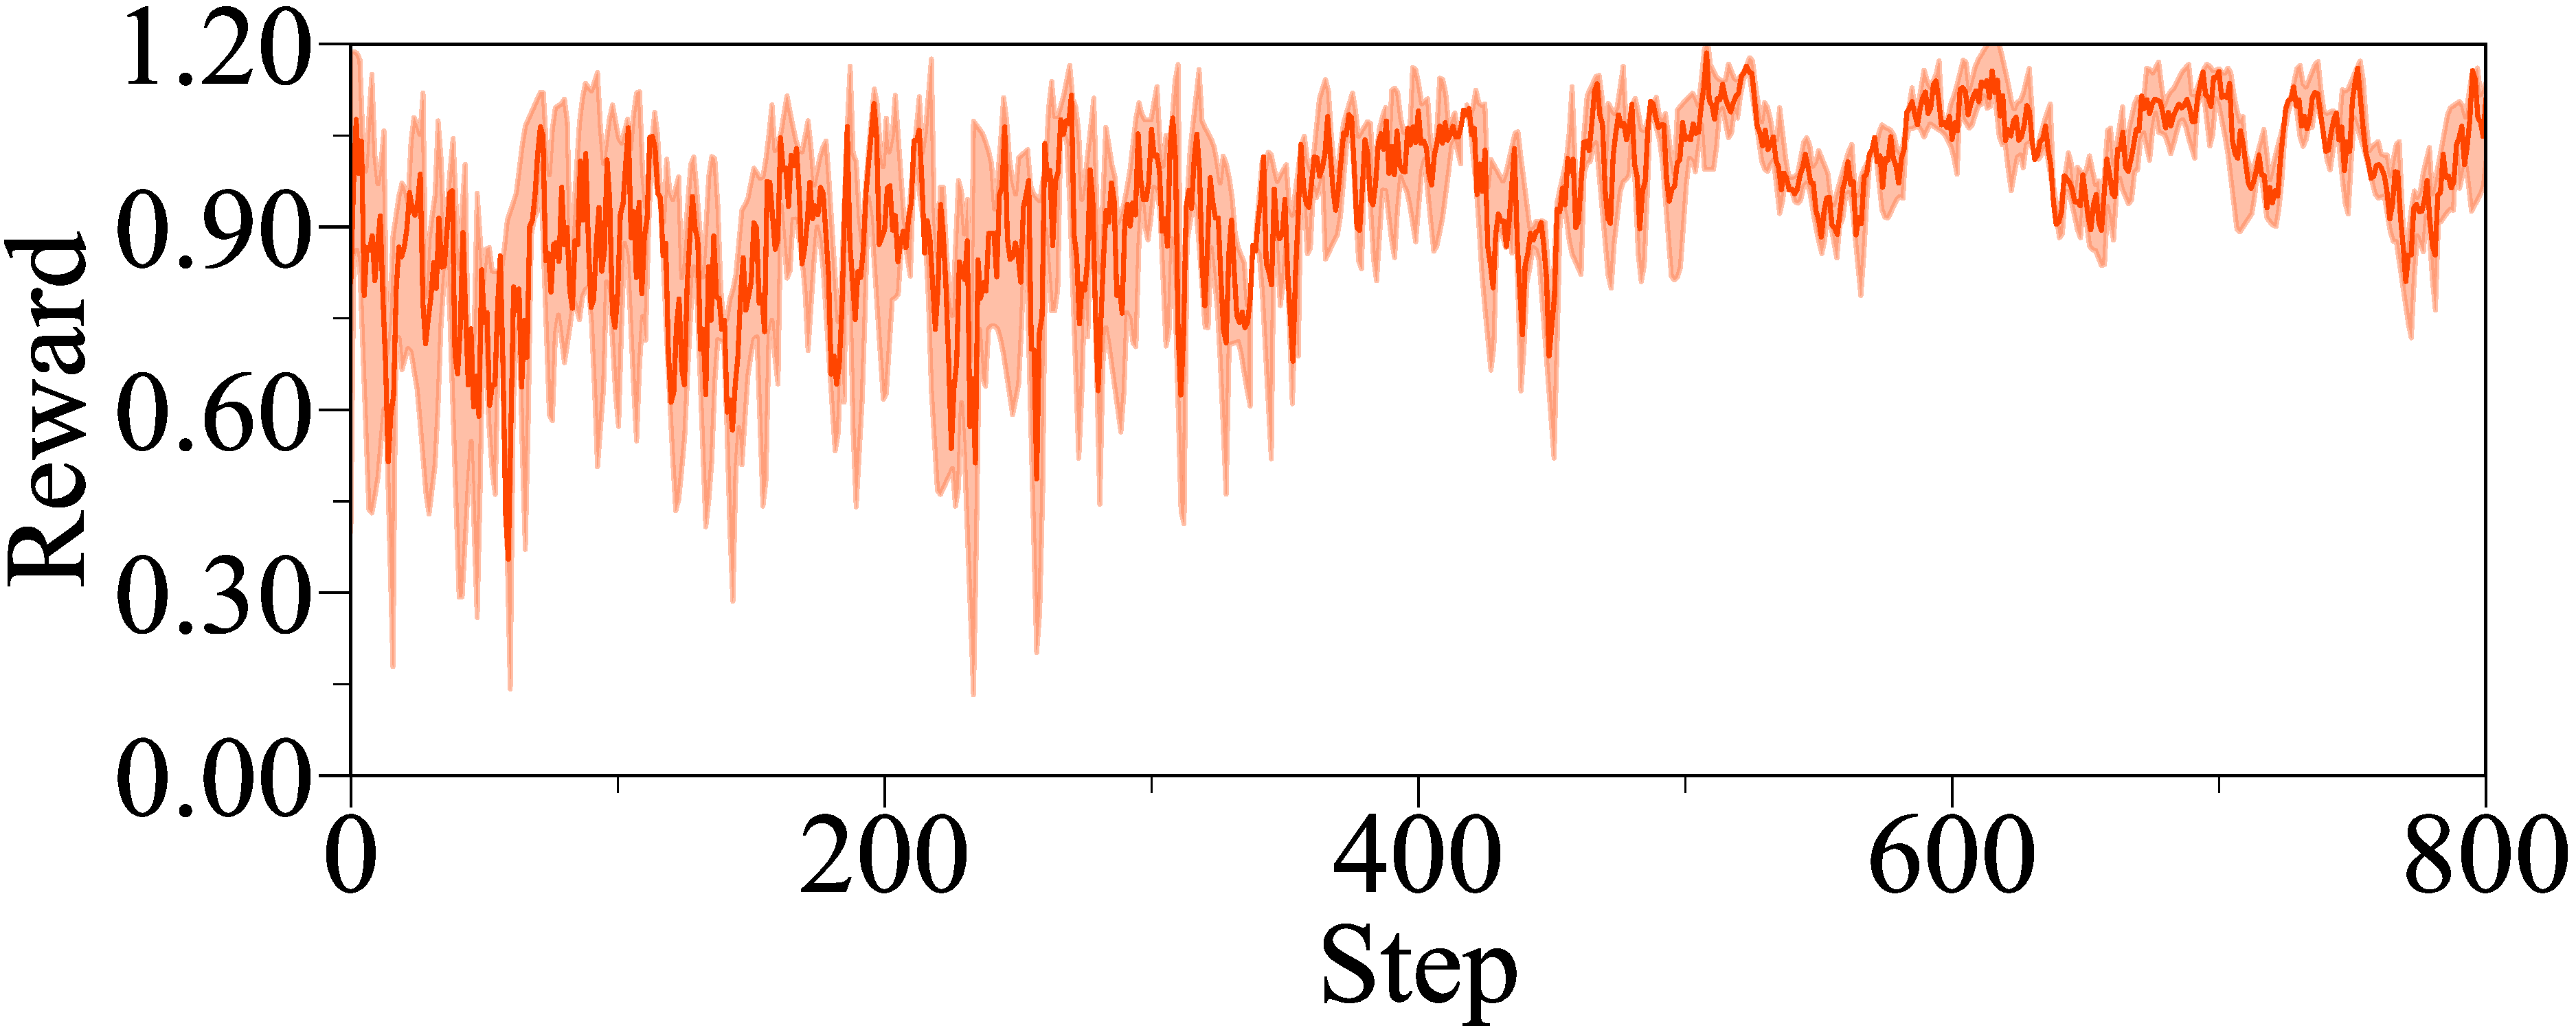
\includegraphics[width=\linewidth]{reward_1.pdf}
        \caption{\black{Training curve of reward}}
        \label{reward-1}
    \end{subfigure}
    \begin{subfigure}{0.9\linewidth} % 第一个子图
        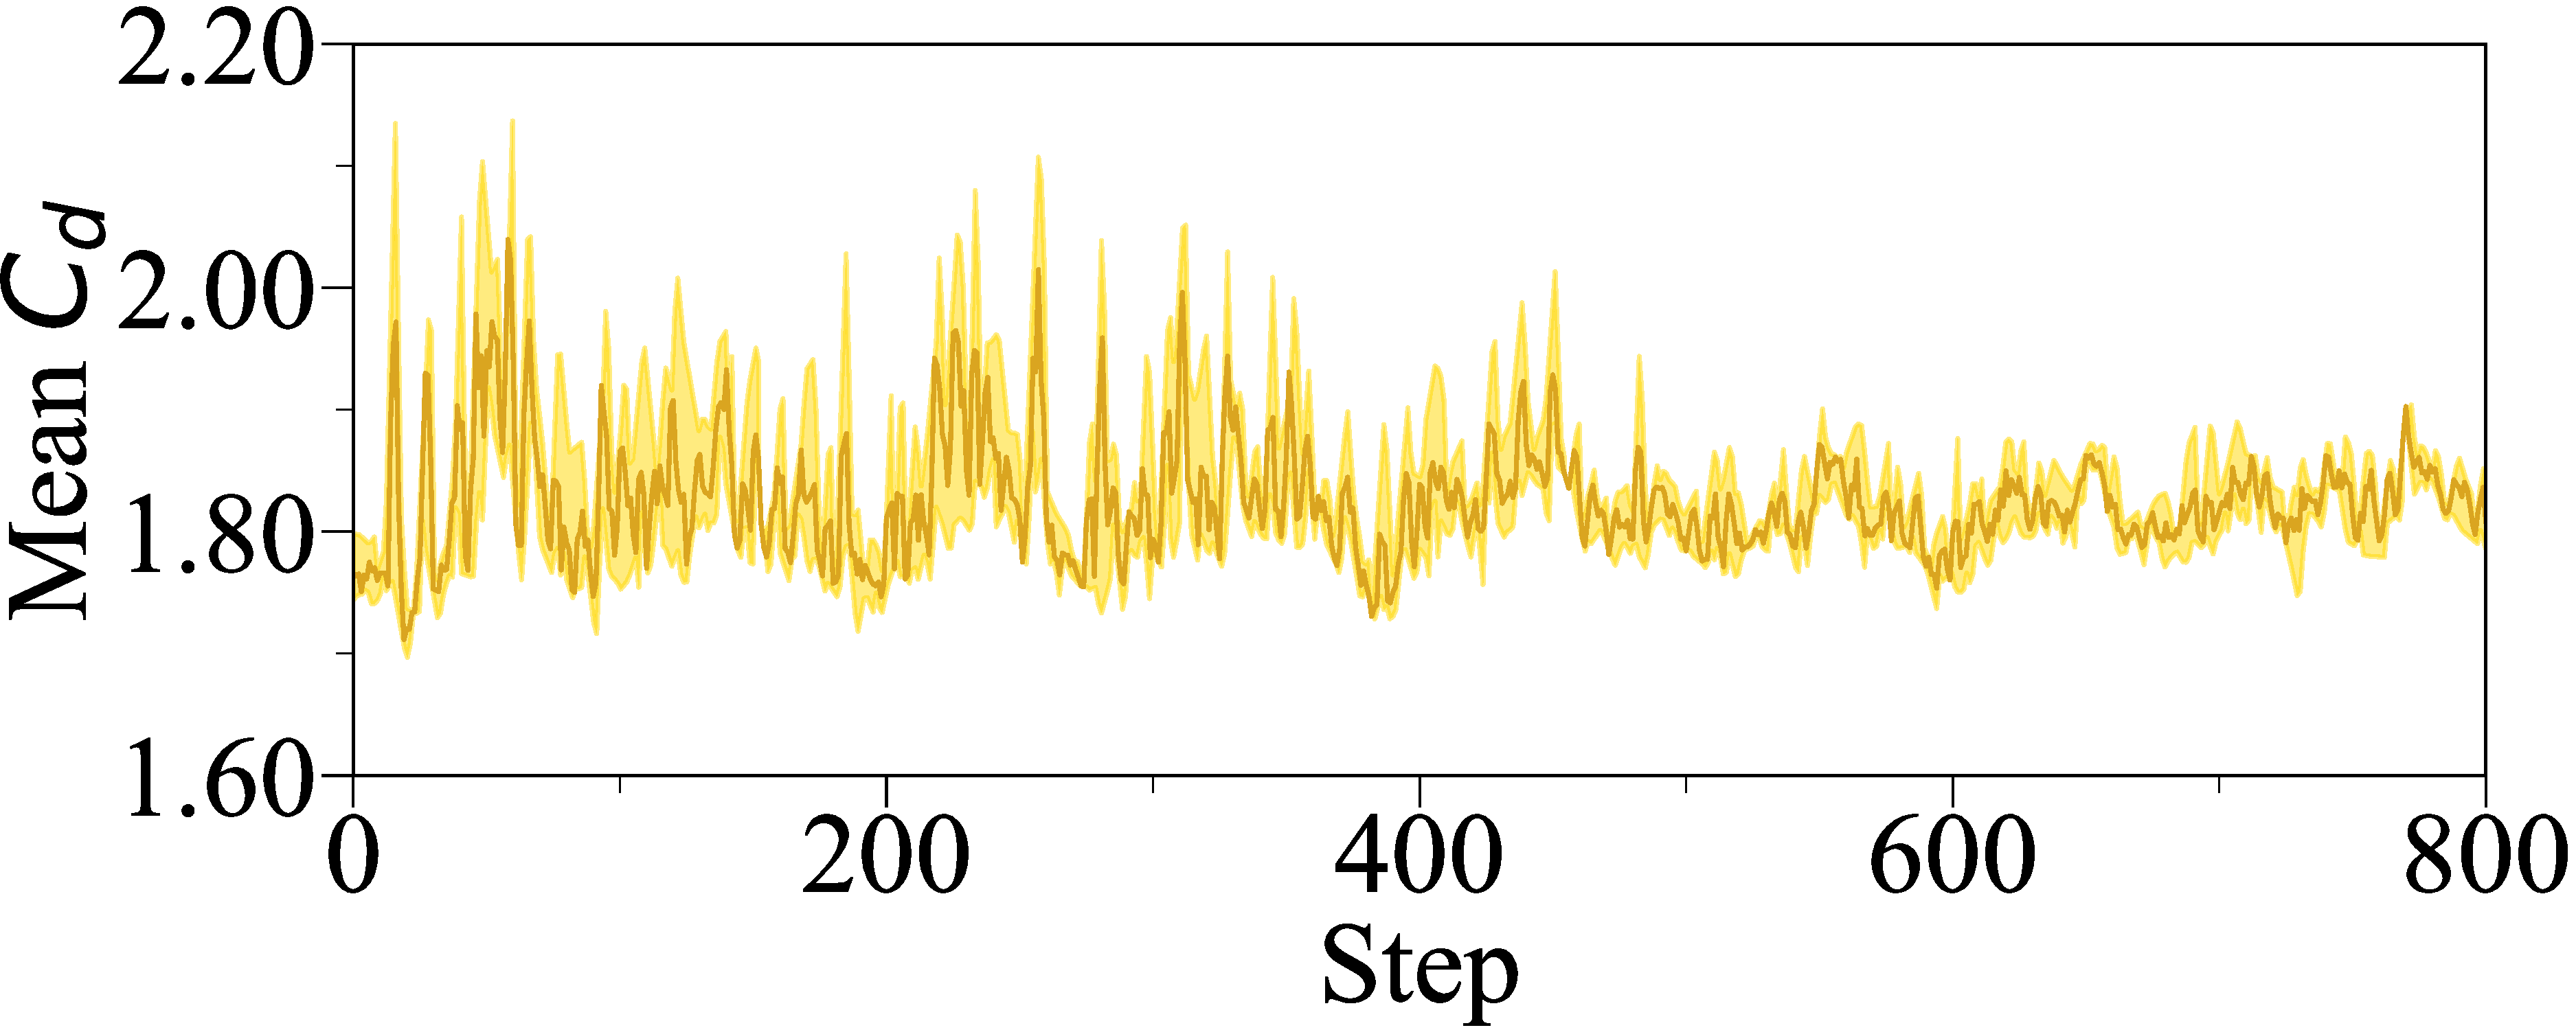
\includegraphics[width=\linewidth]{Cd_1.pdf}
        \caption{\black{Training curve of Mean $C_d$}}
        \label{Cd-1}
    \end{subfigure}
    % \hspace{0.5\linewidth}
    \begin{subfigure}{0.9\linewidth} % 第二个子图
        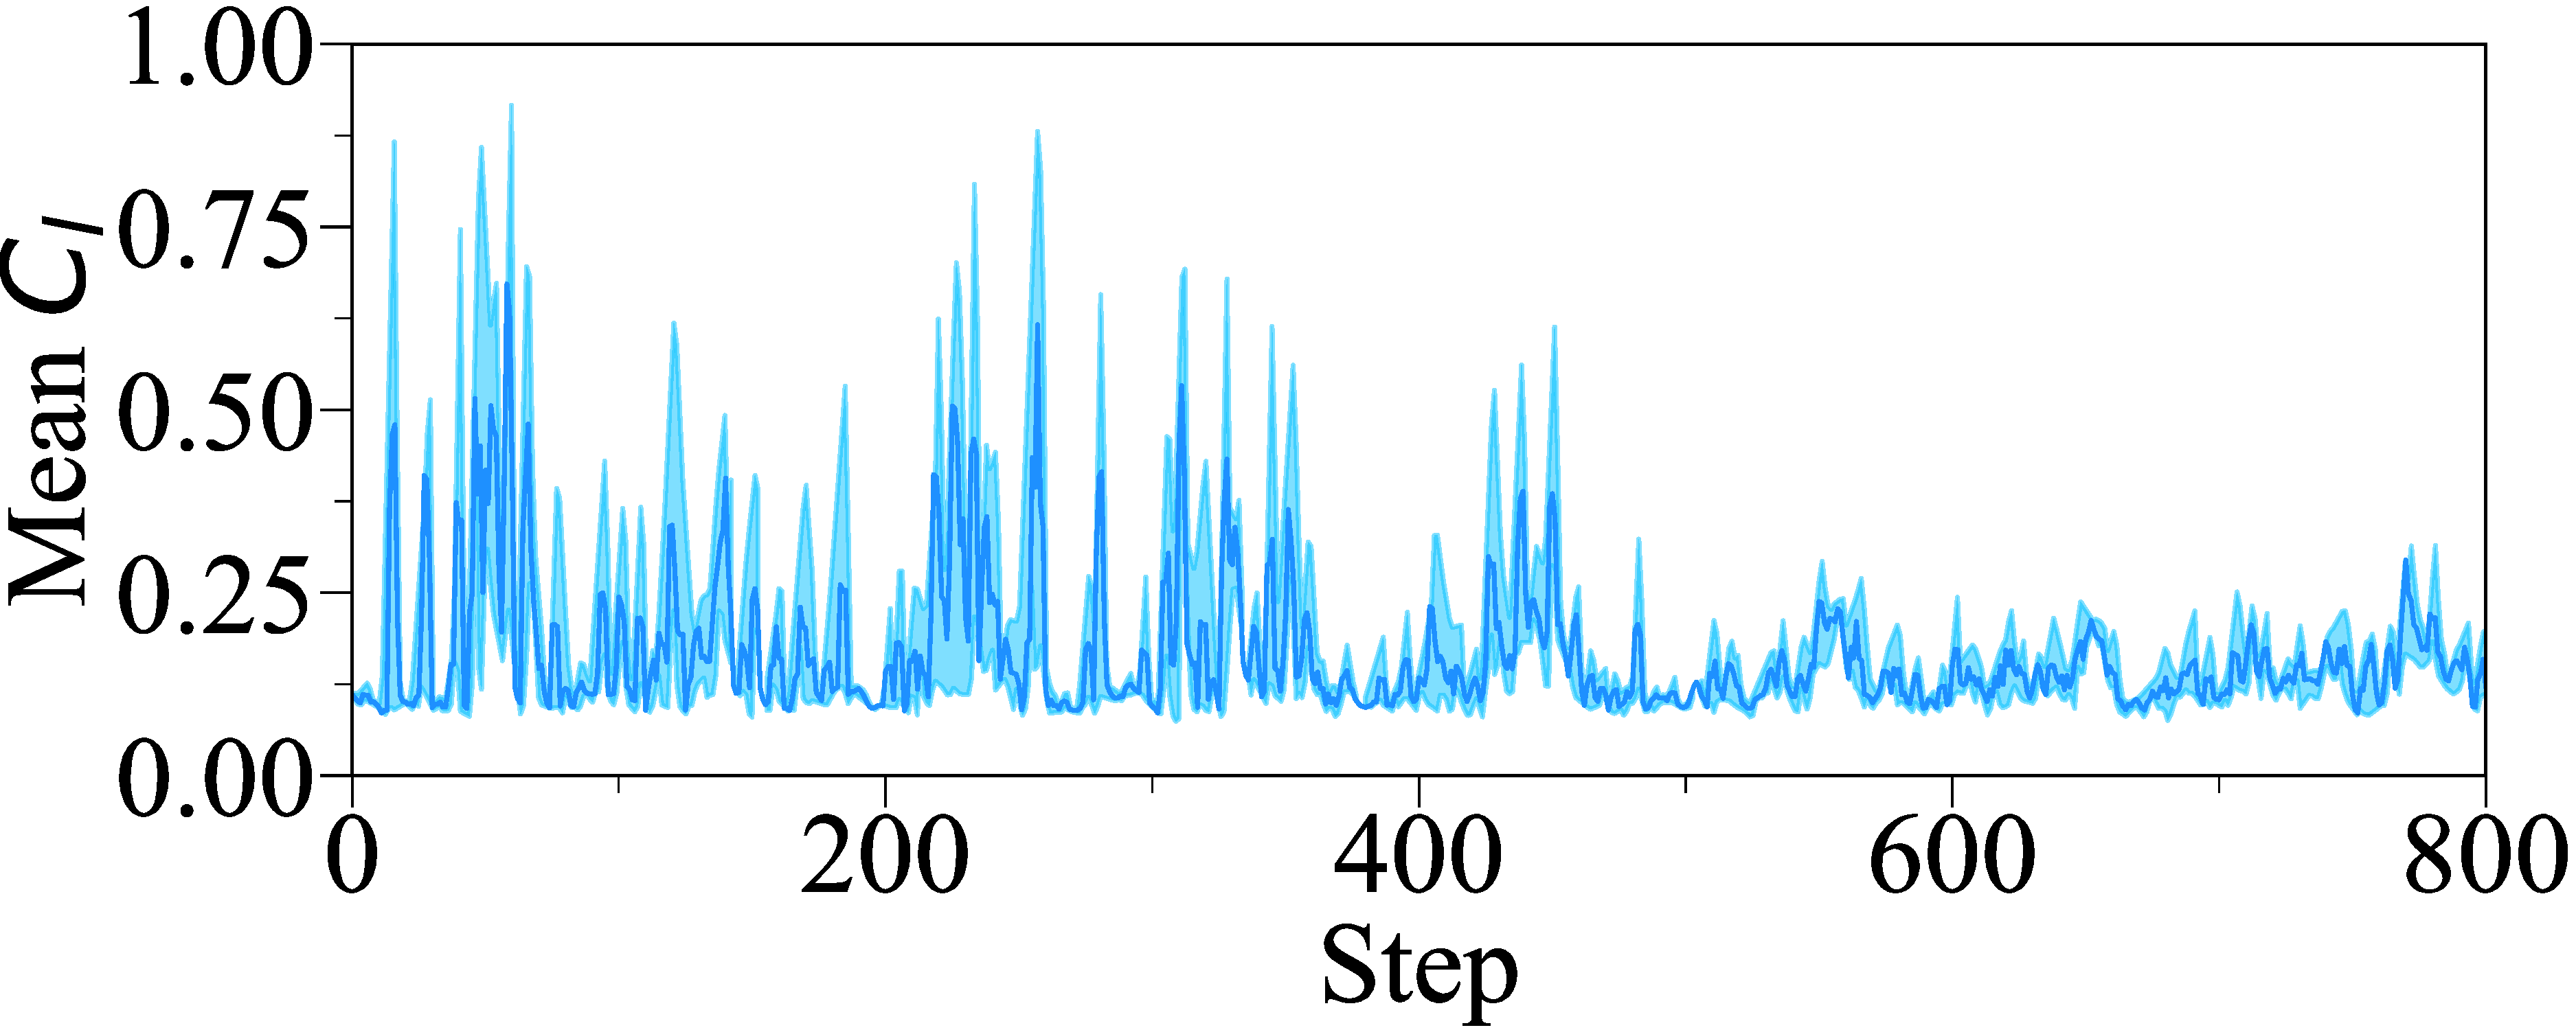
\includegraphics[width=\linewidth]{Cl_1.pdf}
        \caption{\black{Training curve of Std $C_l$}}
        \label{Cl-1}
    \end{subfigure}
    
    \caption{Training curves of reward, mean $C_d$, std $C_l$ in case 1}
    \label{E1 training}
\end{figure}

\begin{figure}
    \centering

    \begin{subfigure}{0.9\linewidth} % 第一个子图
        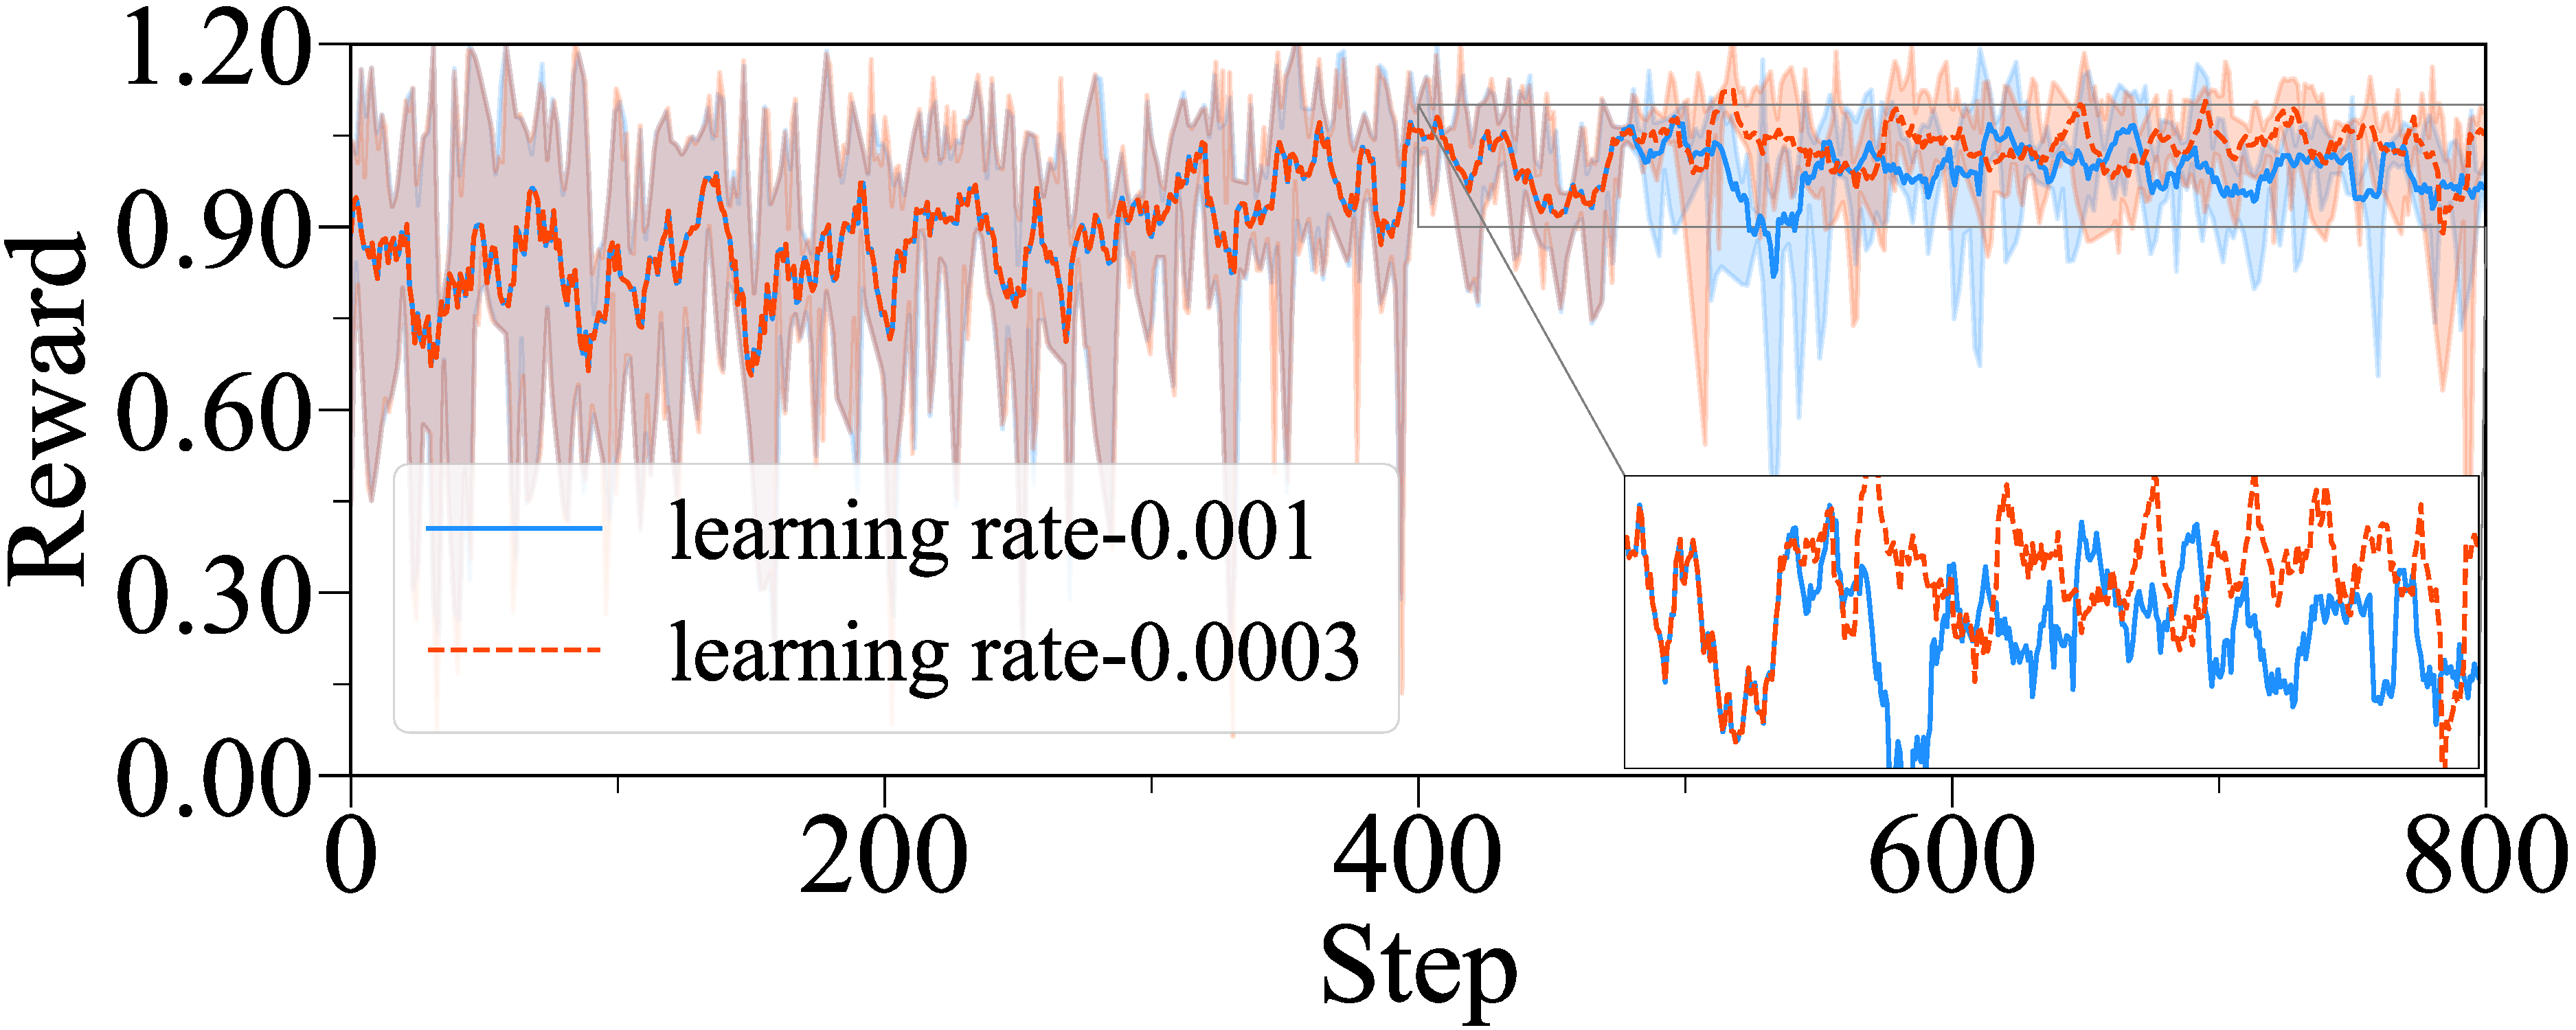
\includegraphics[width=\linewidth]{reward_2.pdf}
        \caption{\black{Training curve of reward}}
        \label{reward-2}
    \end{subfigure}
    \begin{subfigure}{0.9\linewidth} % 第一个子图
        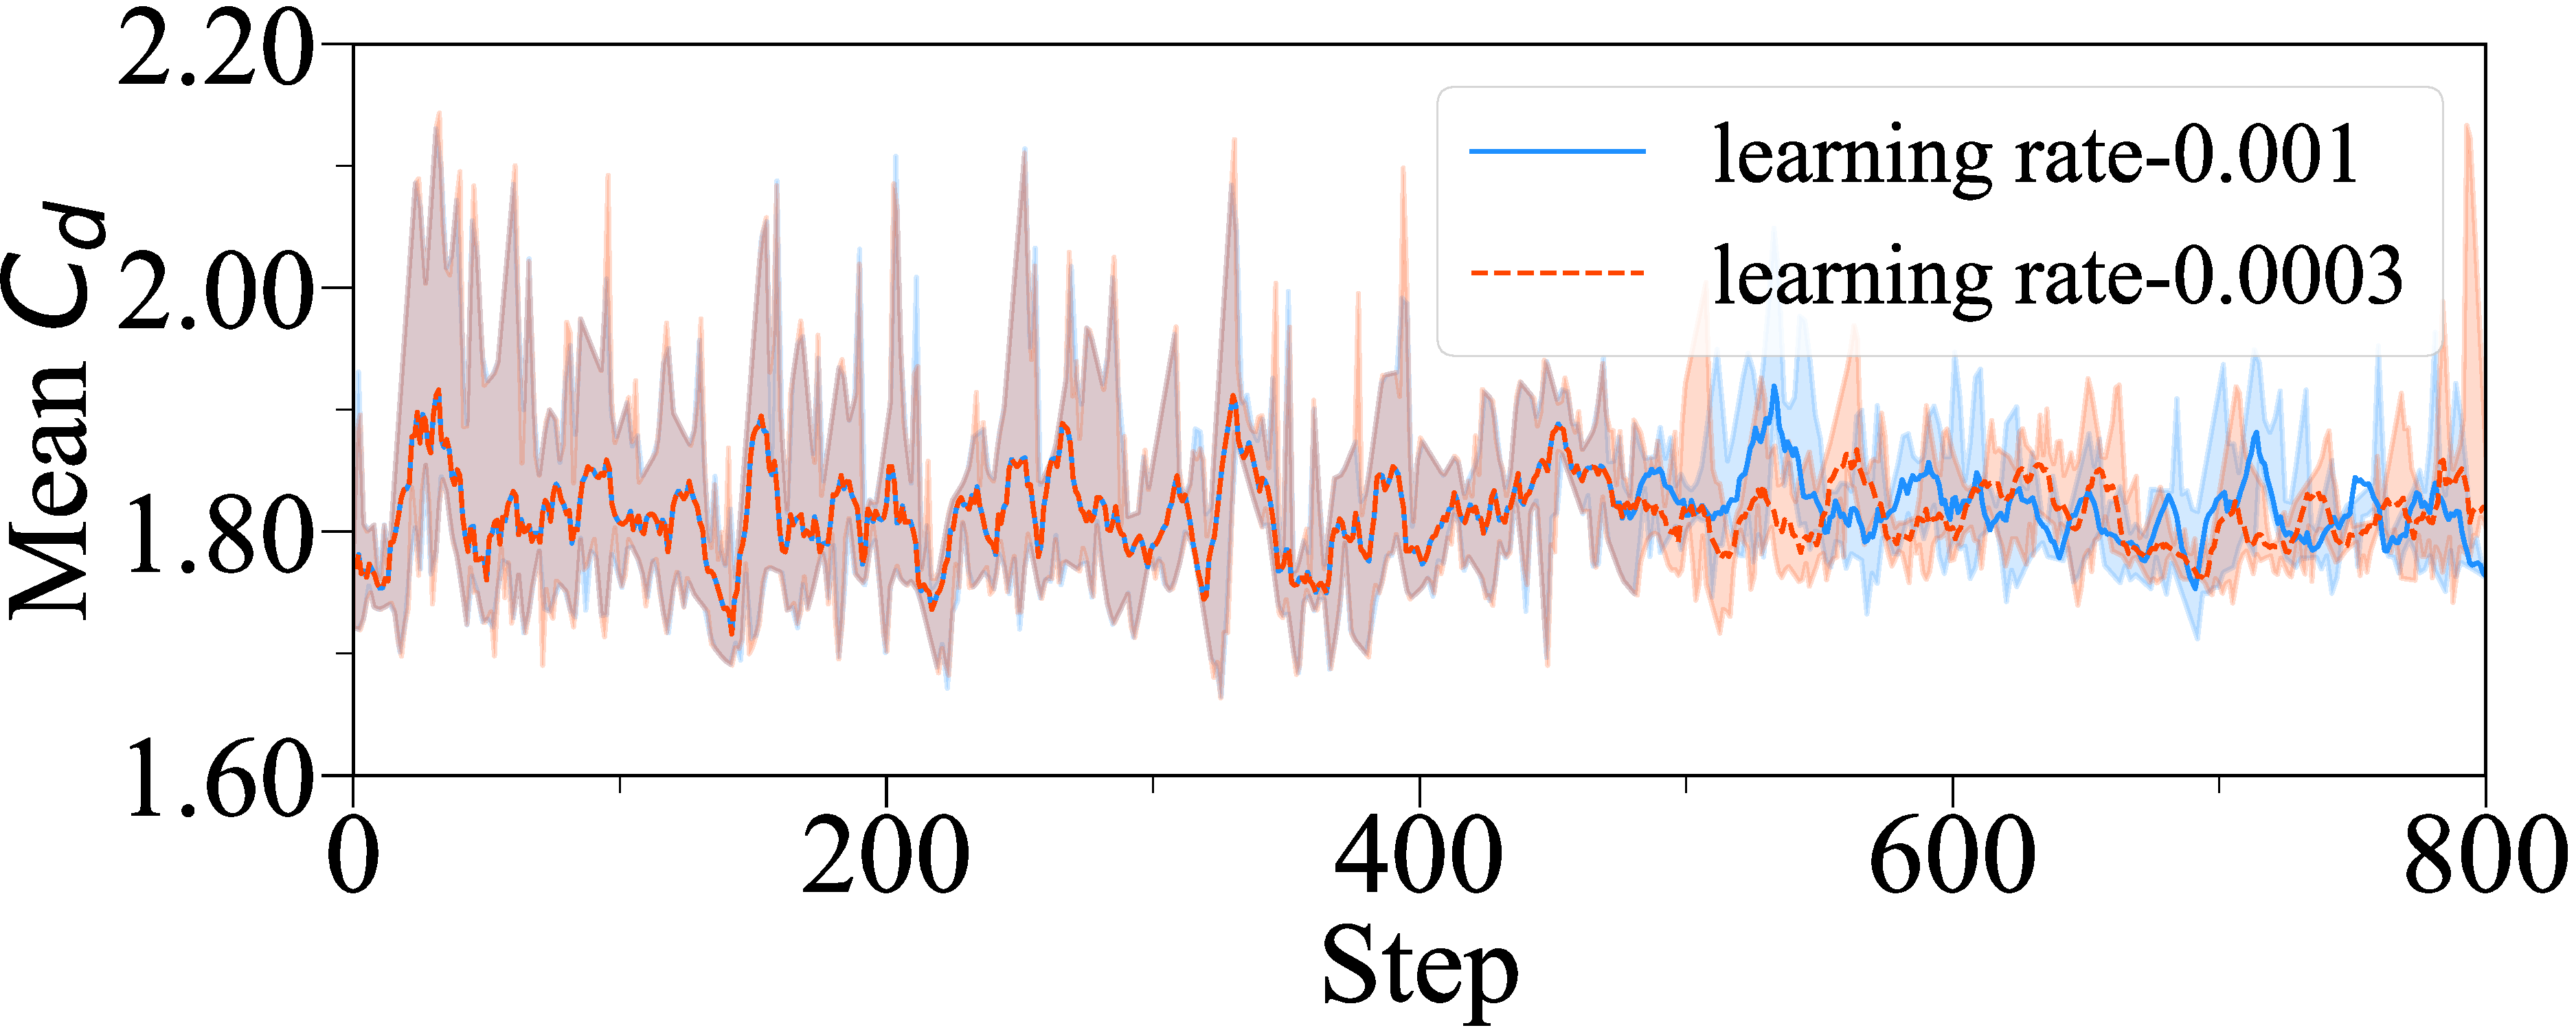
\includegraphics[width=\linewidth]{Cd_2.pdf}
        \caption{\black{Training curve of Mean $C_d$}}
        \label{Cd-2}
    \end{subfigure}
    % \hspace{0.5\linewidth}
    \begin{subfigure}{0.9\linewidth} % 第二个子图
        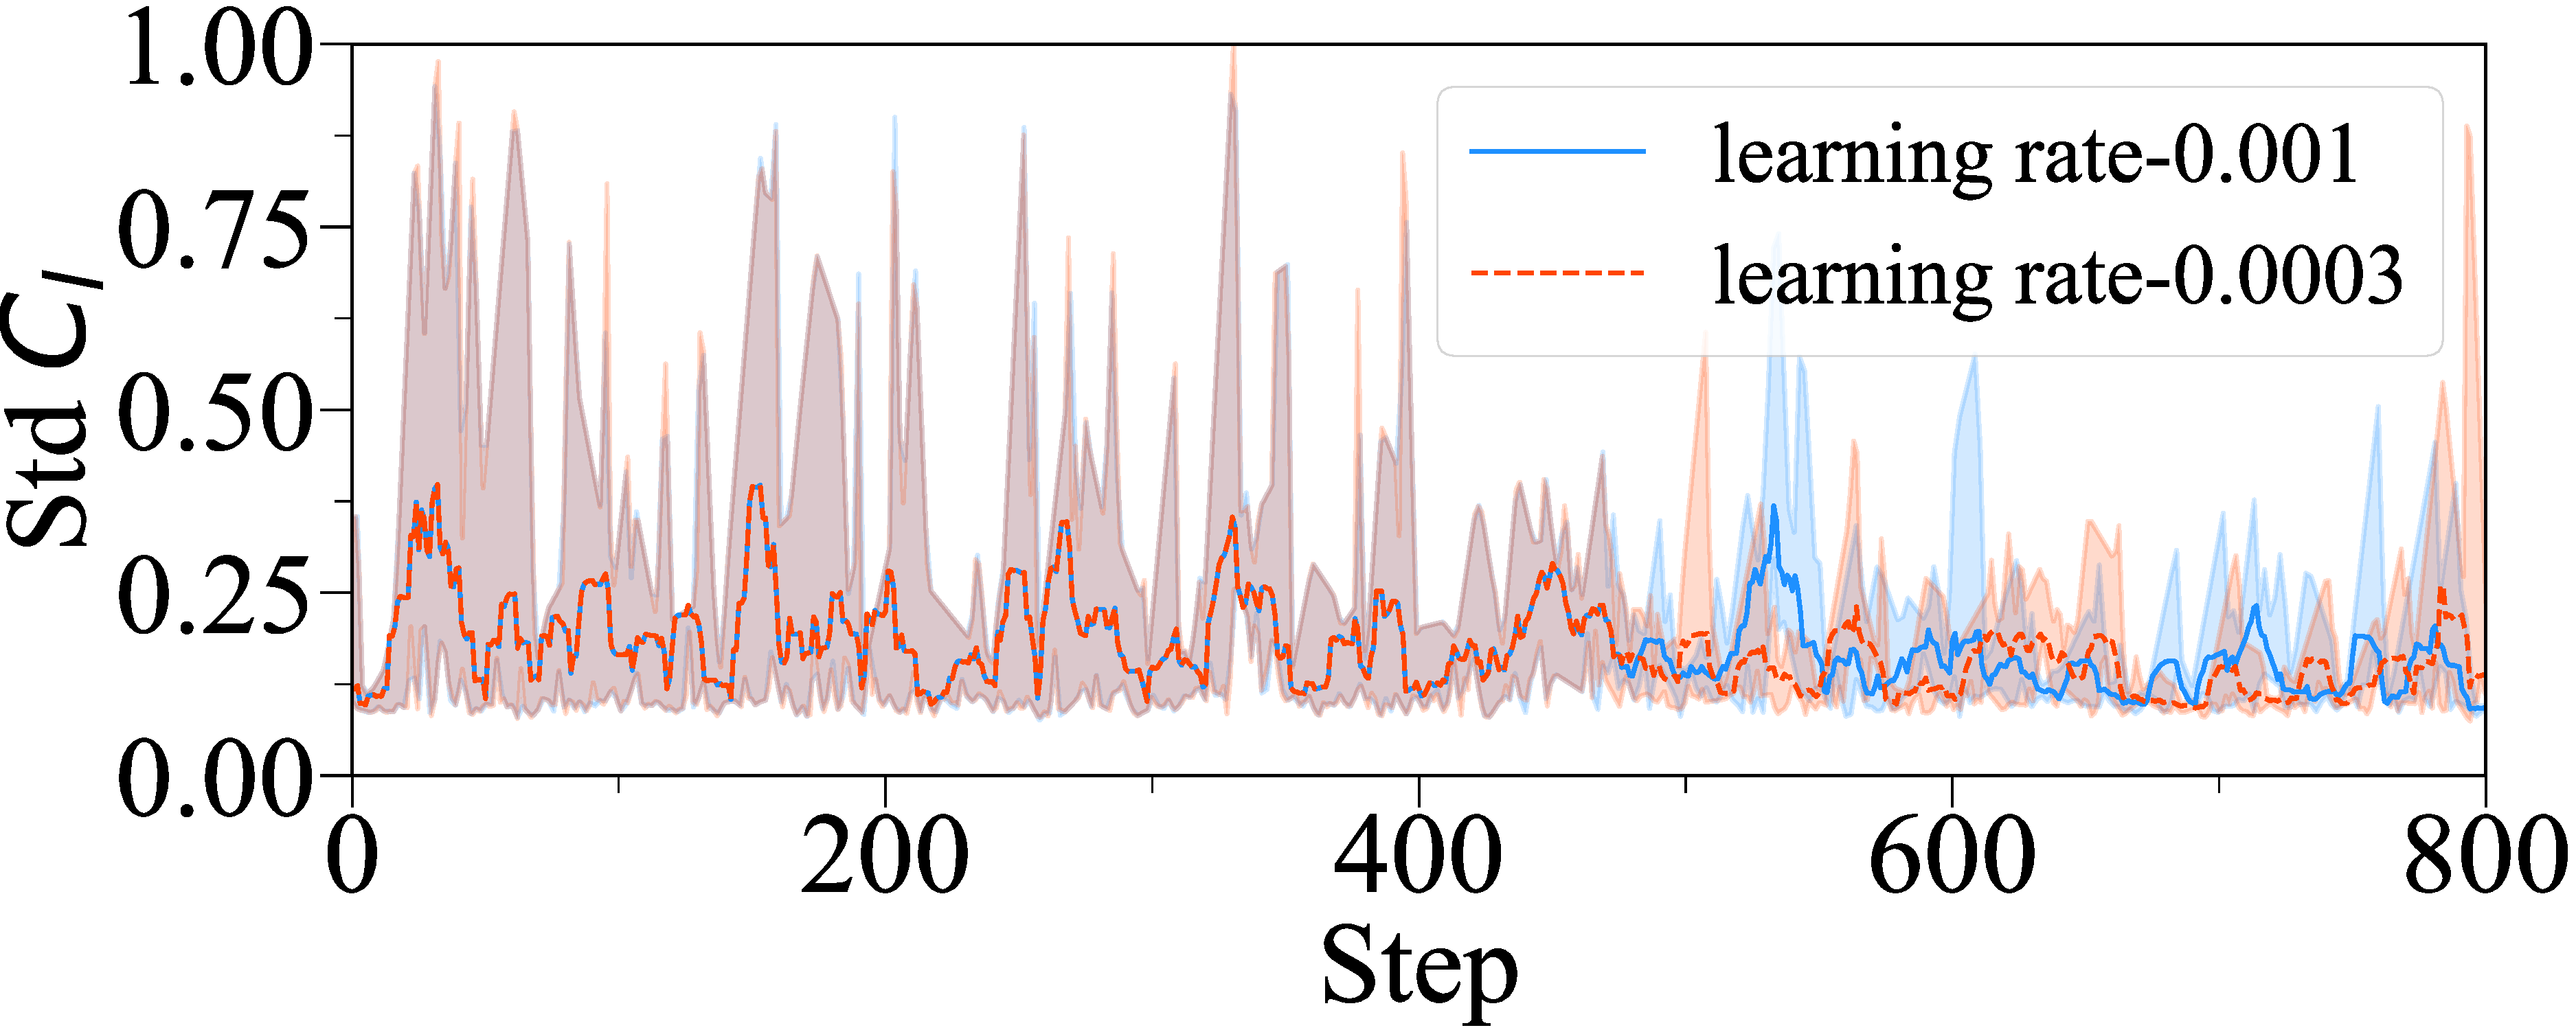
\includegraphics[width=\linewidth]{Cl_2.pdf}
        \caption{\black{Training curve of Std $C_l$}}
        \label{Cl-2}
    \end{subfigure}
    
    \caption{Training curves of reward, mean $C_d$, std $C_l$ in case 2. Using a smaller learning rate of 0.0003 at step 520 can get better results.}
    \label{E2 training}
\end{figure}

\begin{figure}
    \centering

    \begin{subfigure}{0.9\linewidth} % 第一个子图
        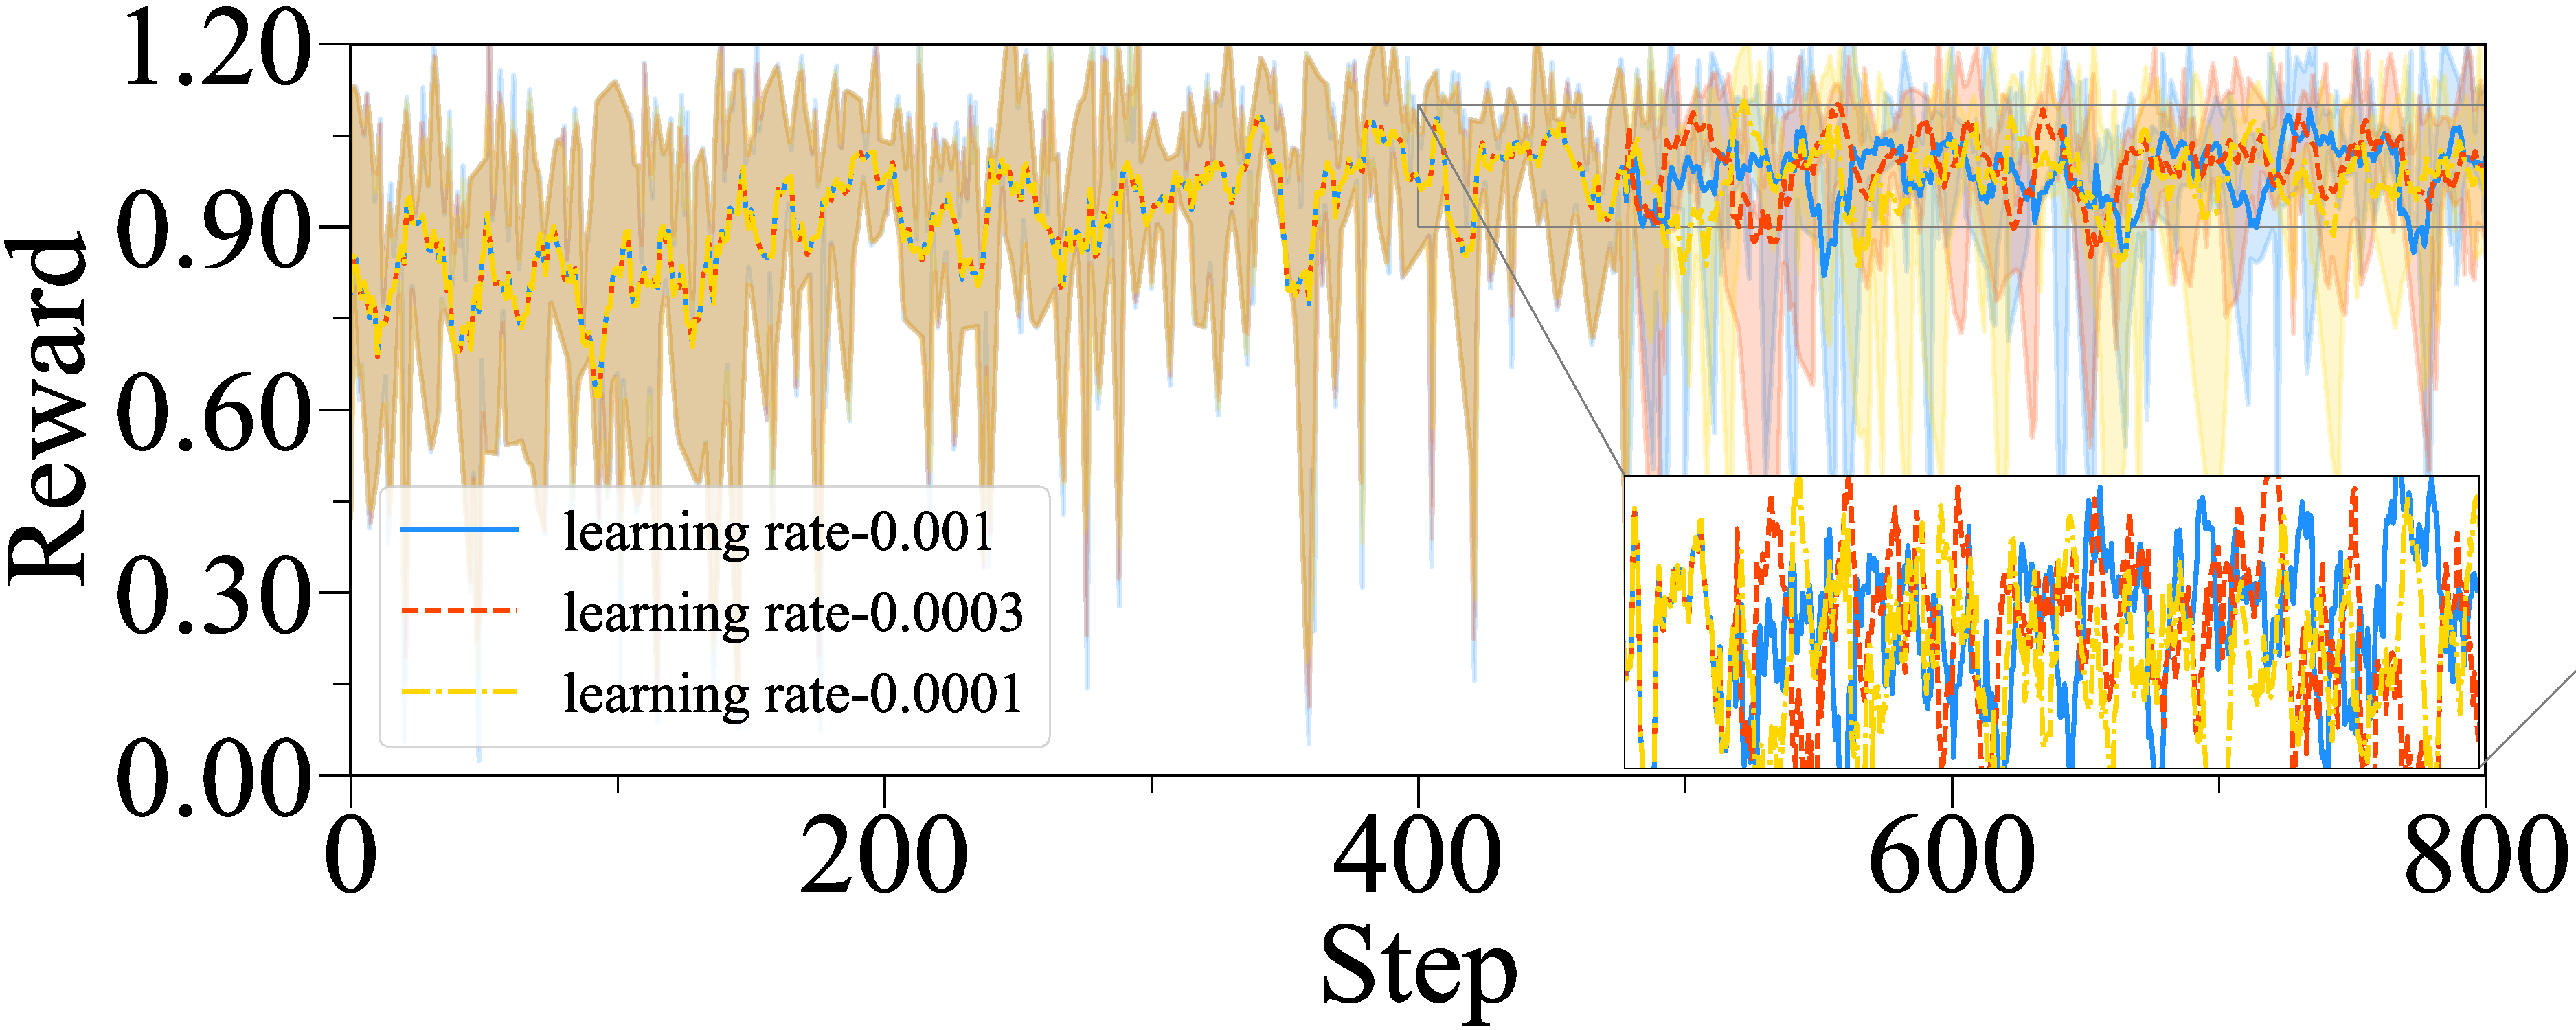
\includegraphics[width=\linewidth]{reward_3.pdf}
        \caption{\black{Training curve of reward}}
        \label{reward_3}
    \end{subfigure}
    \begin{subfigure}{0.9\linewidth} % 第一个子图
        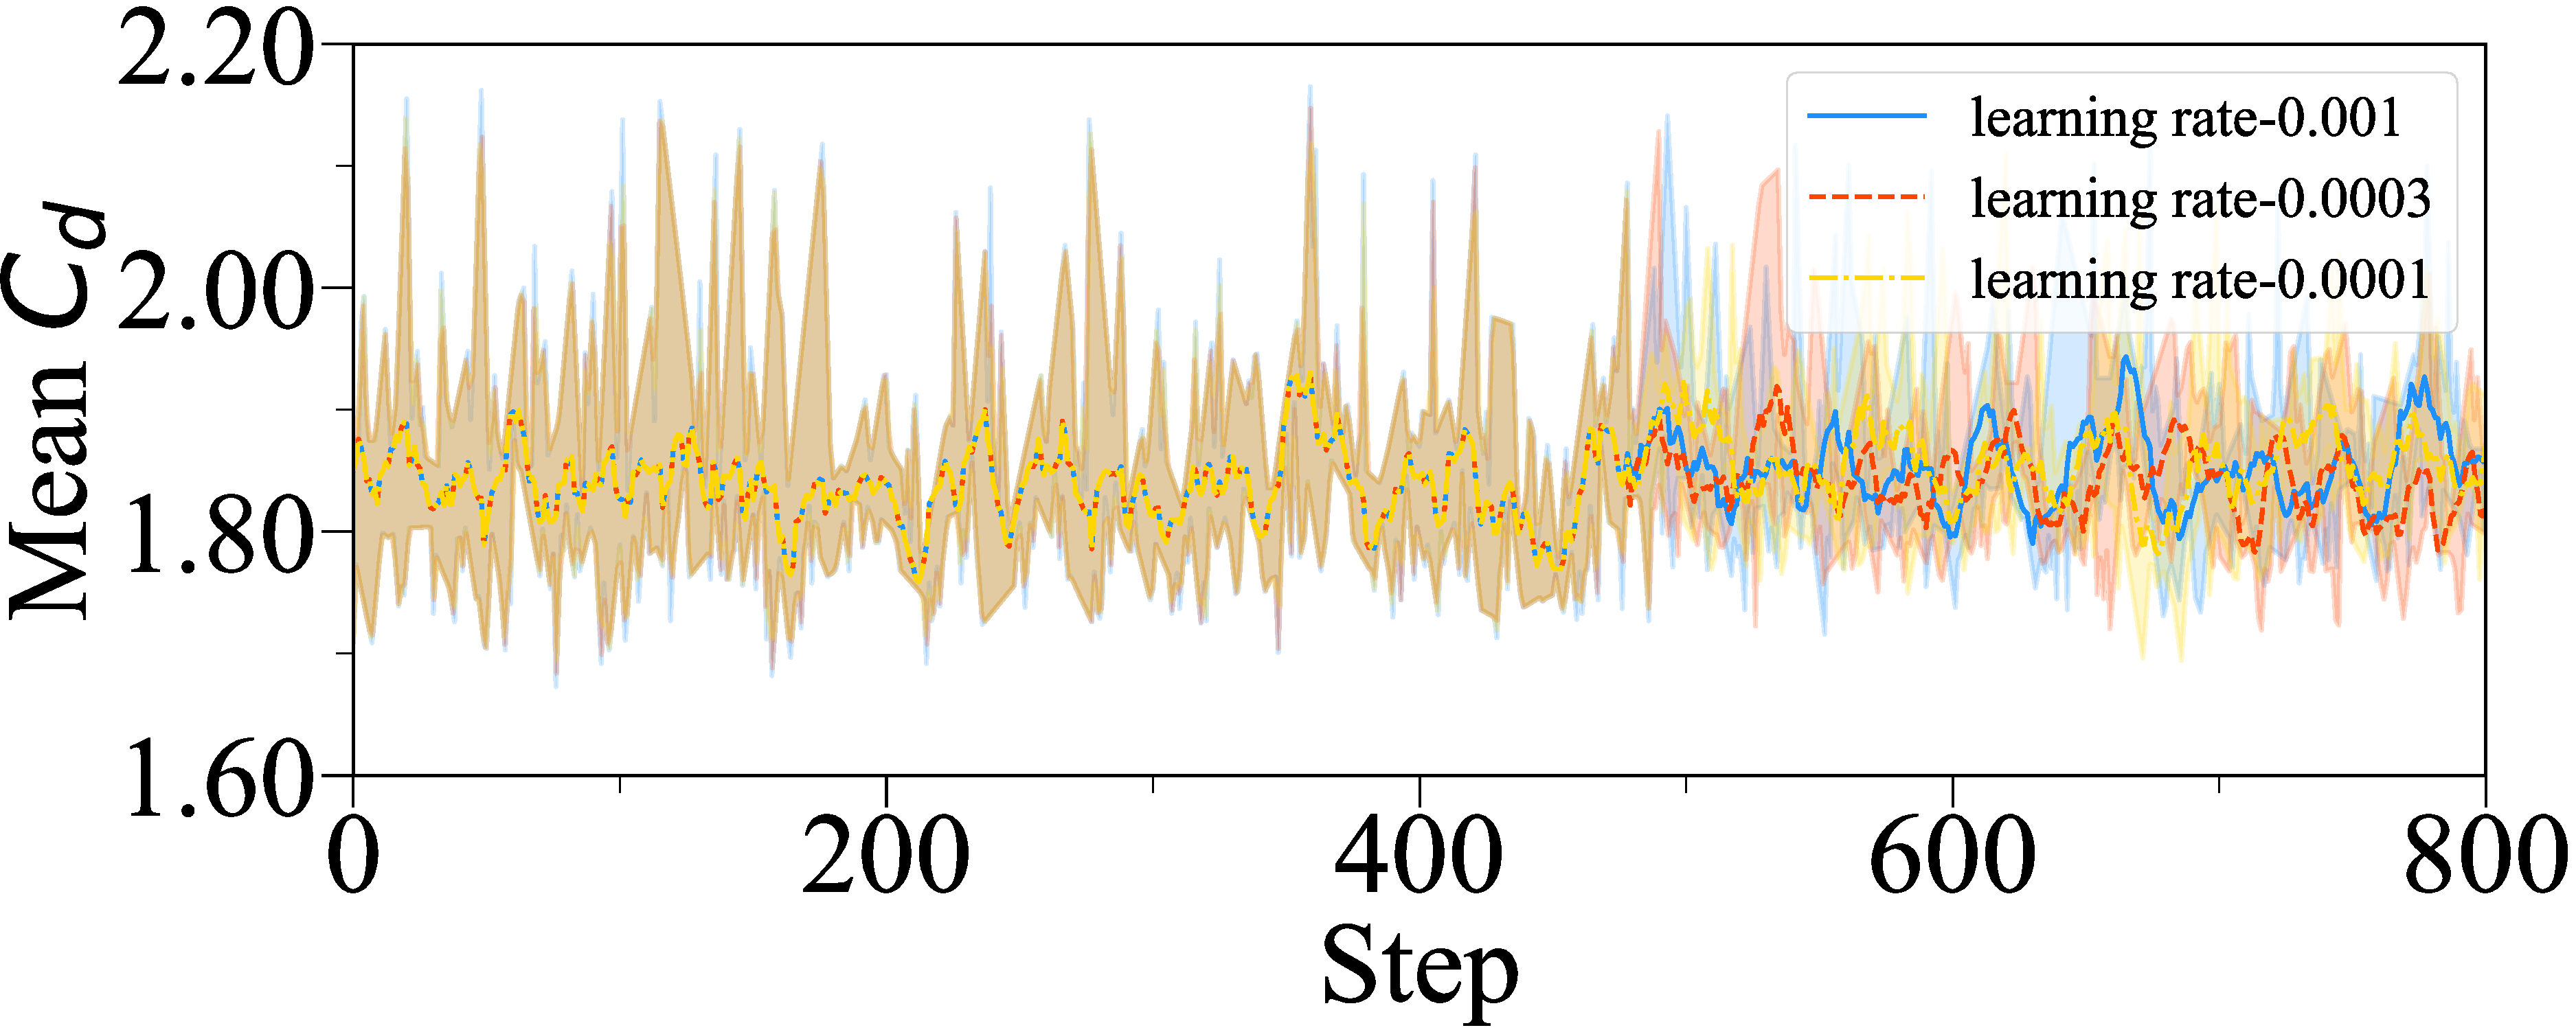
\includegraphics[width=\linewidth]{Cd_3.pdf}
        \caption{\black{Training curve of Mean $C_d$}}
        \label{Cd_3}
    \end{subfigure}
    % \hspace{0.5\linewidth}
    \begin{subfigure}{0.9\linewidth} % 第二个子图
        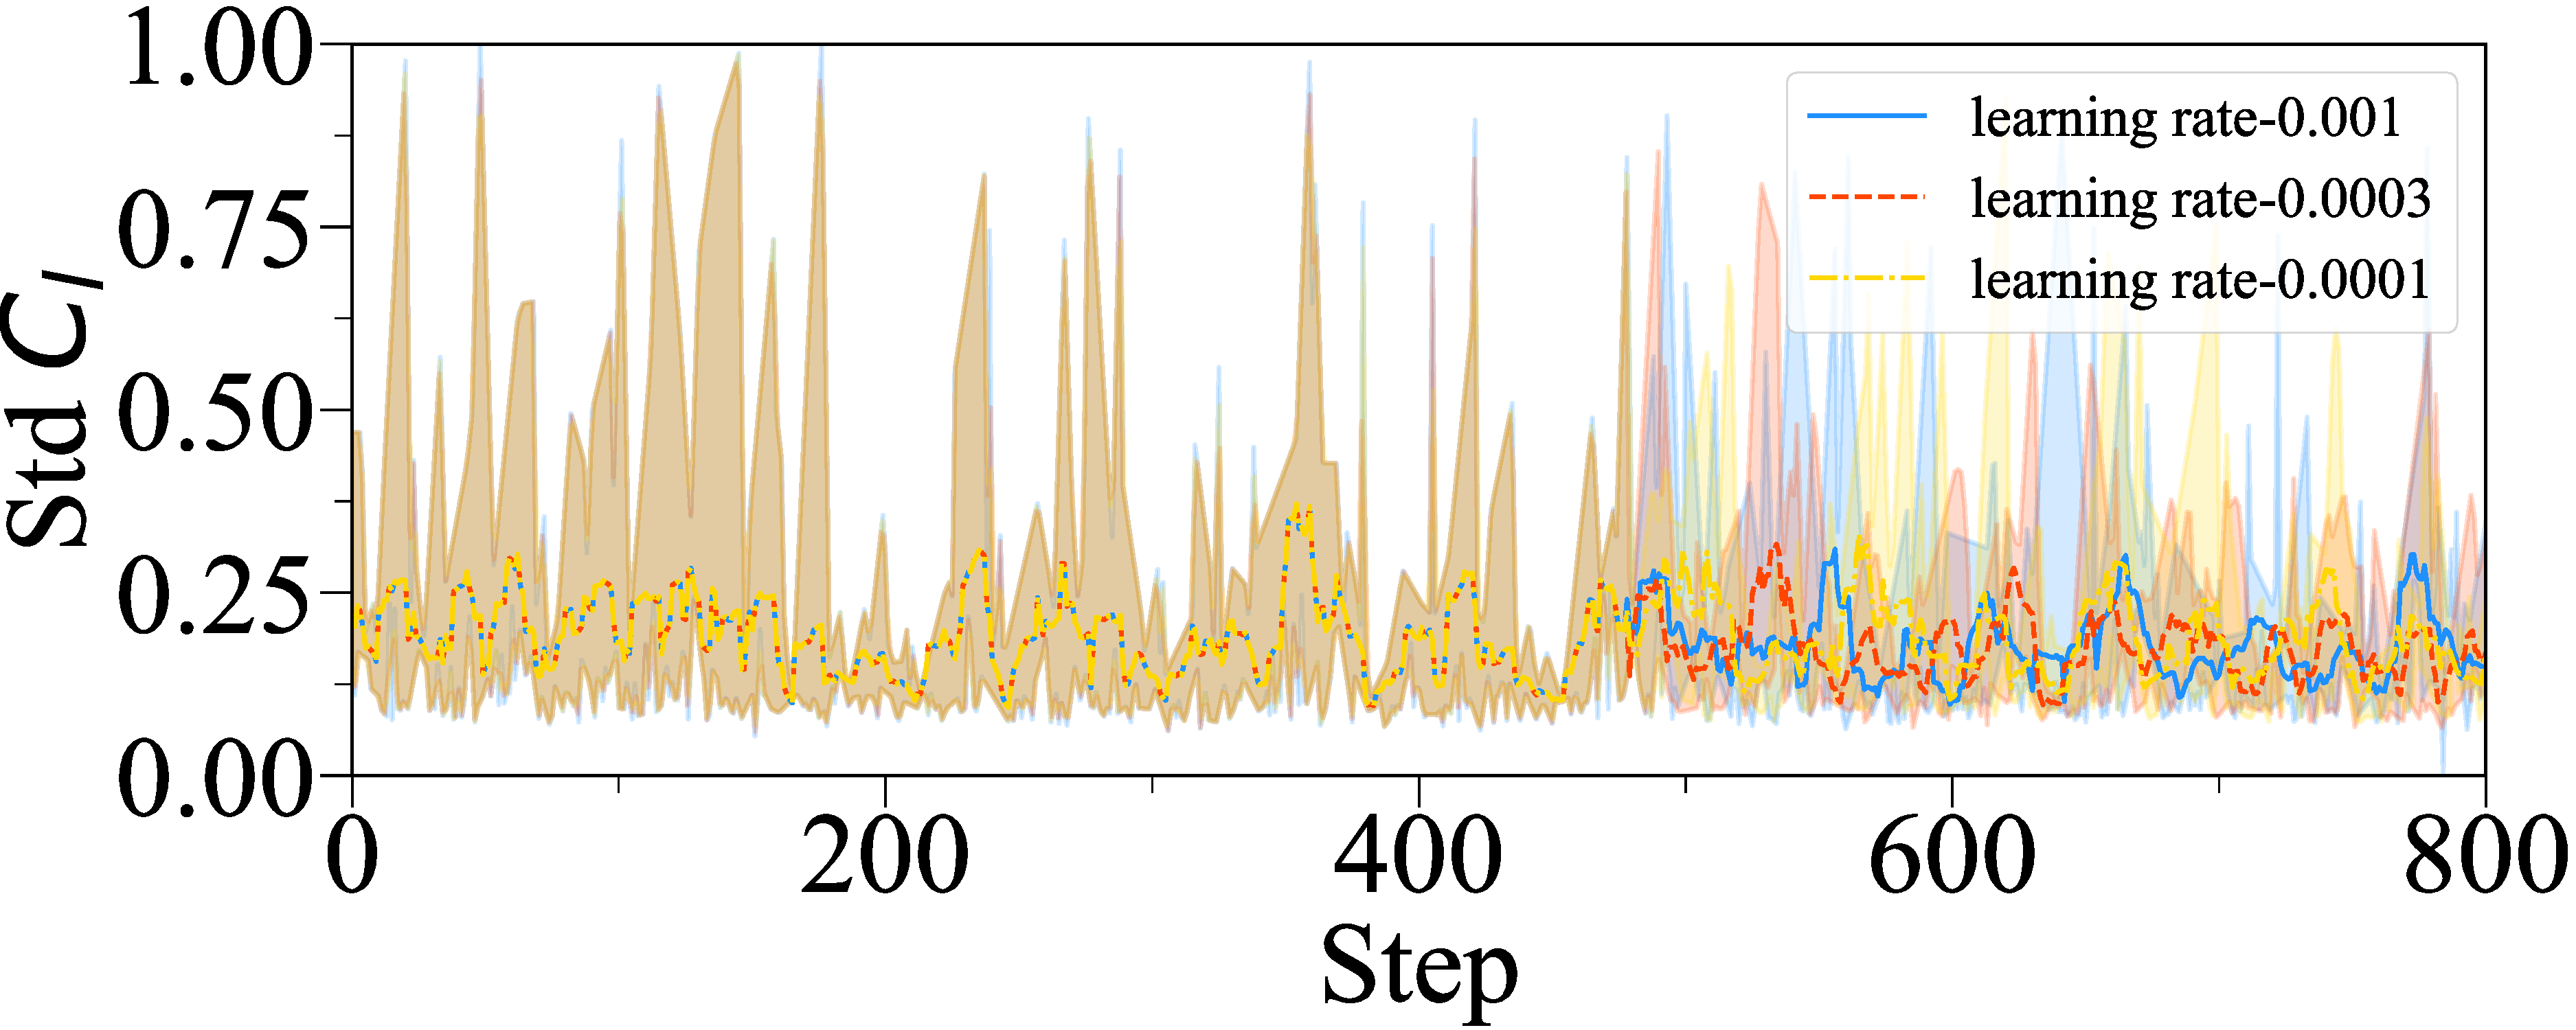
\includegraphics[width=\linewidth]{Cl_3.pdf}
        \caption{\black{Training curve of Std $C_l$}}
        \label{Cl_3}
    \end{subfigure}
    
    \caption{Training curves of reward, mean $C_d$, std $C_l$ in case 3.The results of all three learning rates have similar effects.}
    \label{E3 training}
\end{figure}

\begin{figure}
    \centering

    \begin{subfigure}{0.9\linewidth} % 第一个子图
        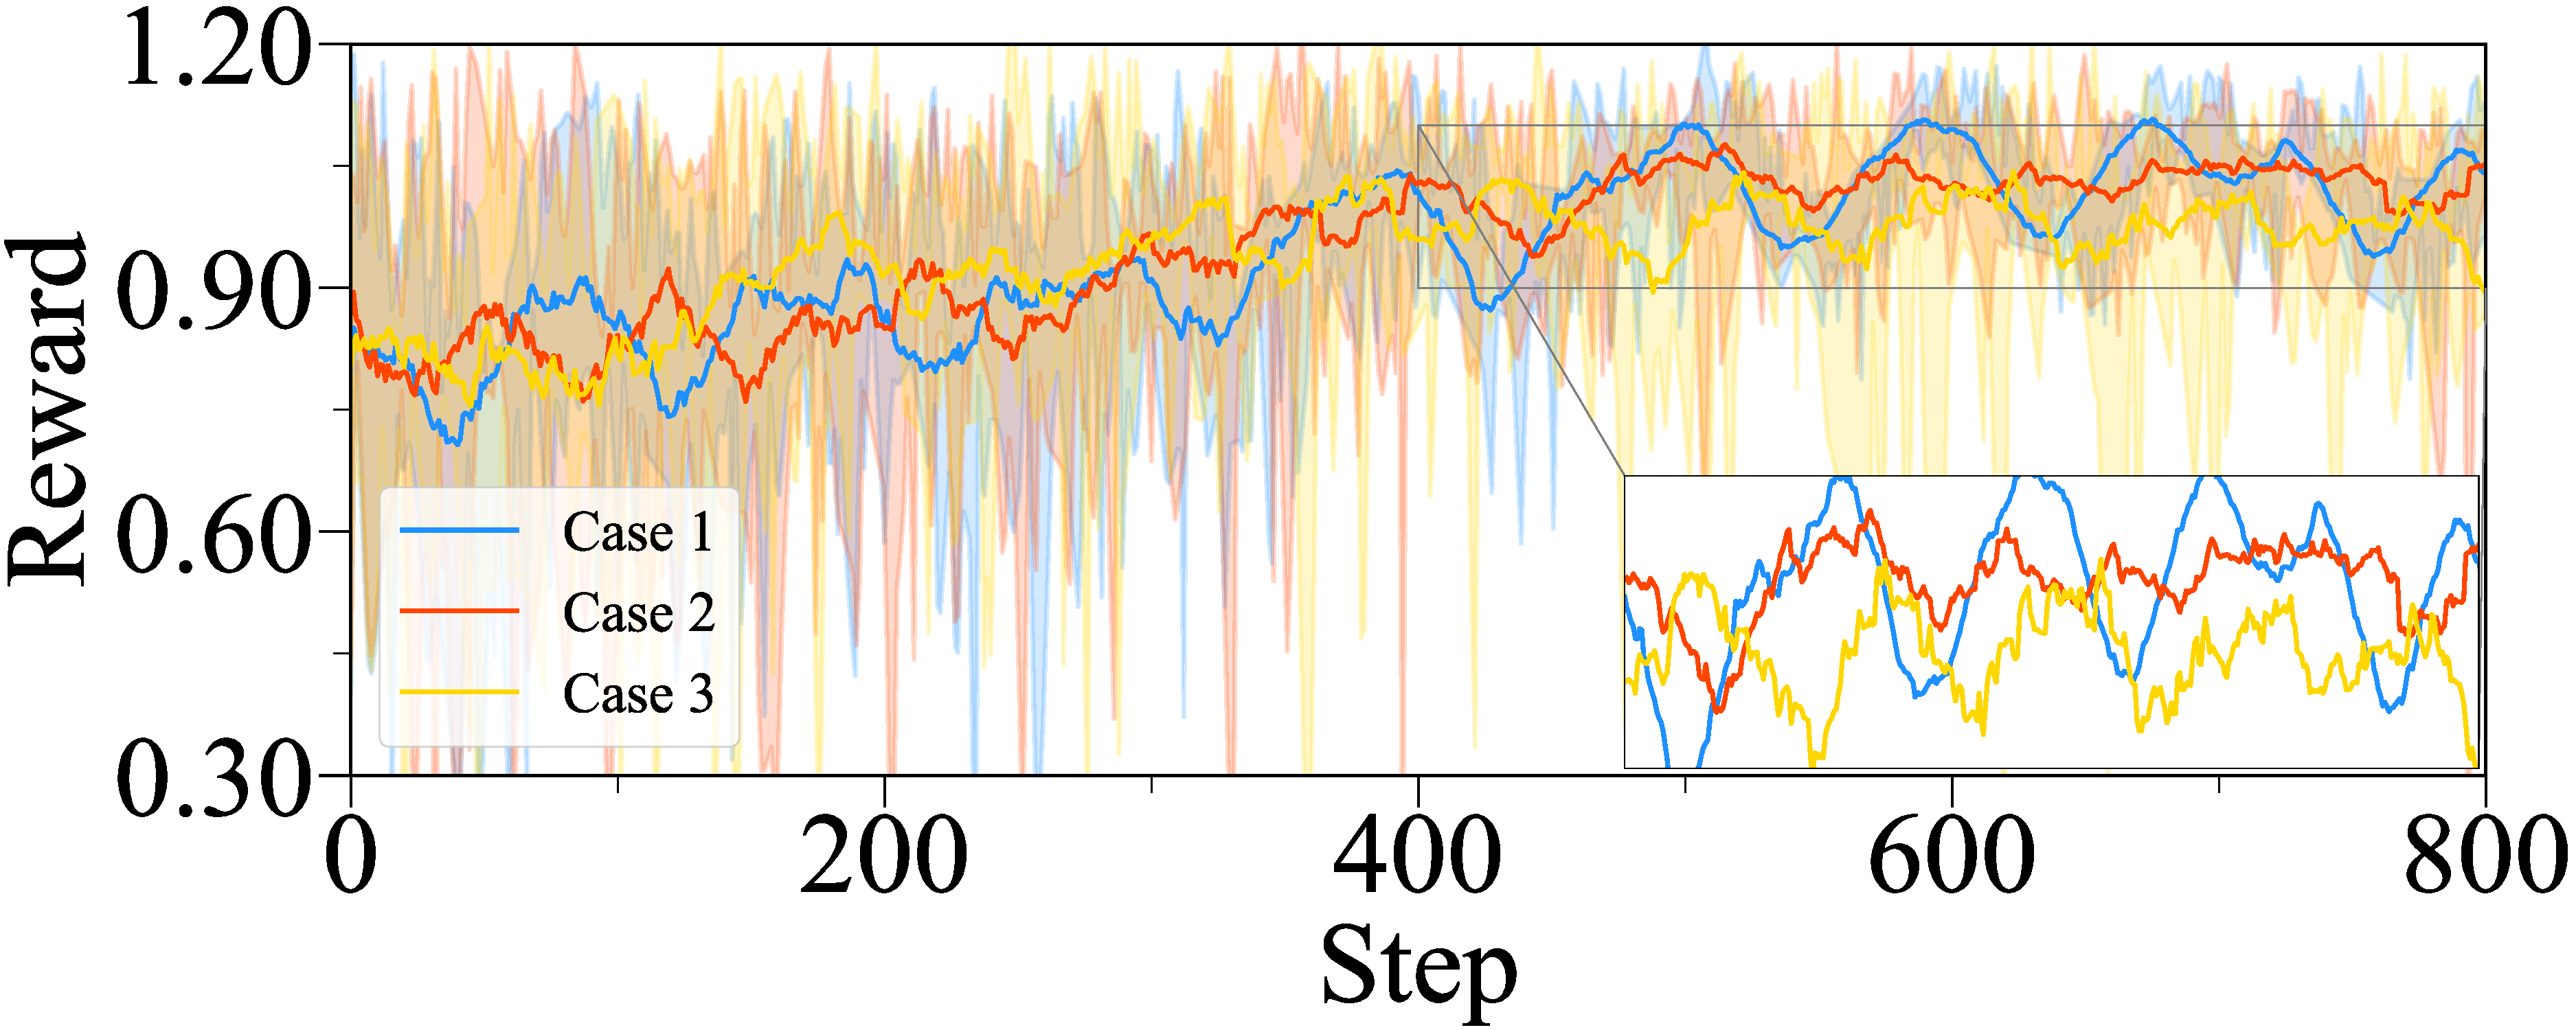
\includegraphics[width=\linewidth]{reward_1_2_3.pdf}
        \caption{\black{Training curve of reward}}
        \label{reward_1_2_3}
    \end{subfigure}
    \begin{subfigure}{0.9\linewidth} % 第一个子图
        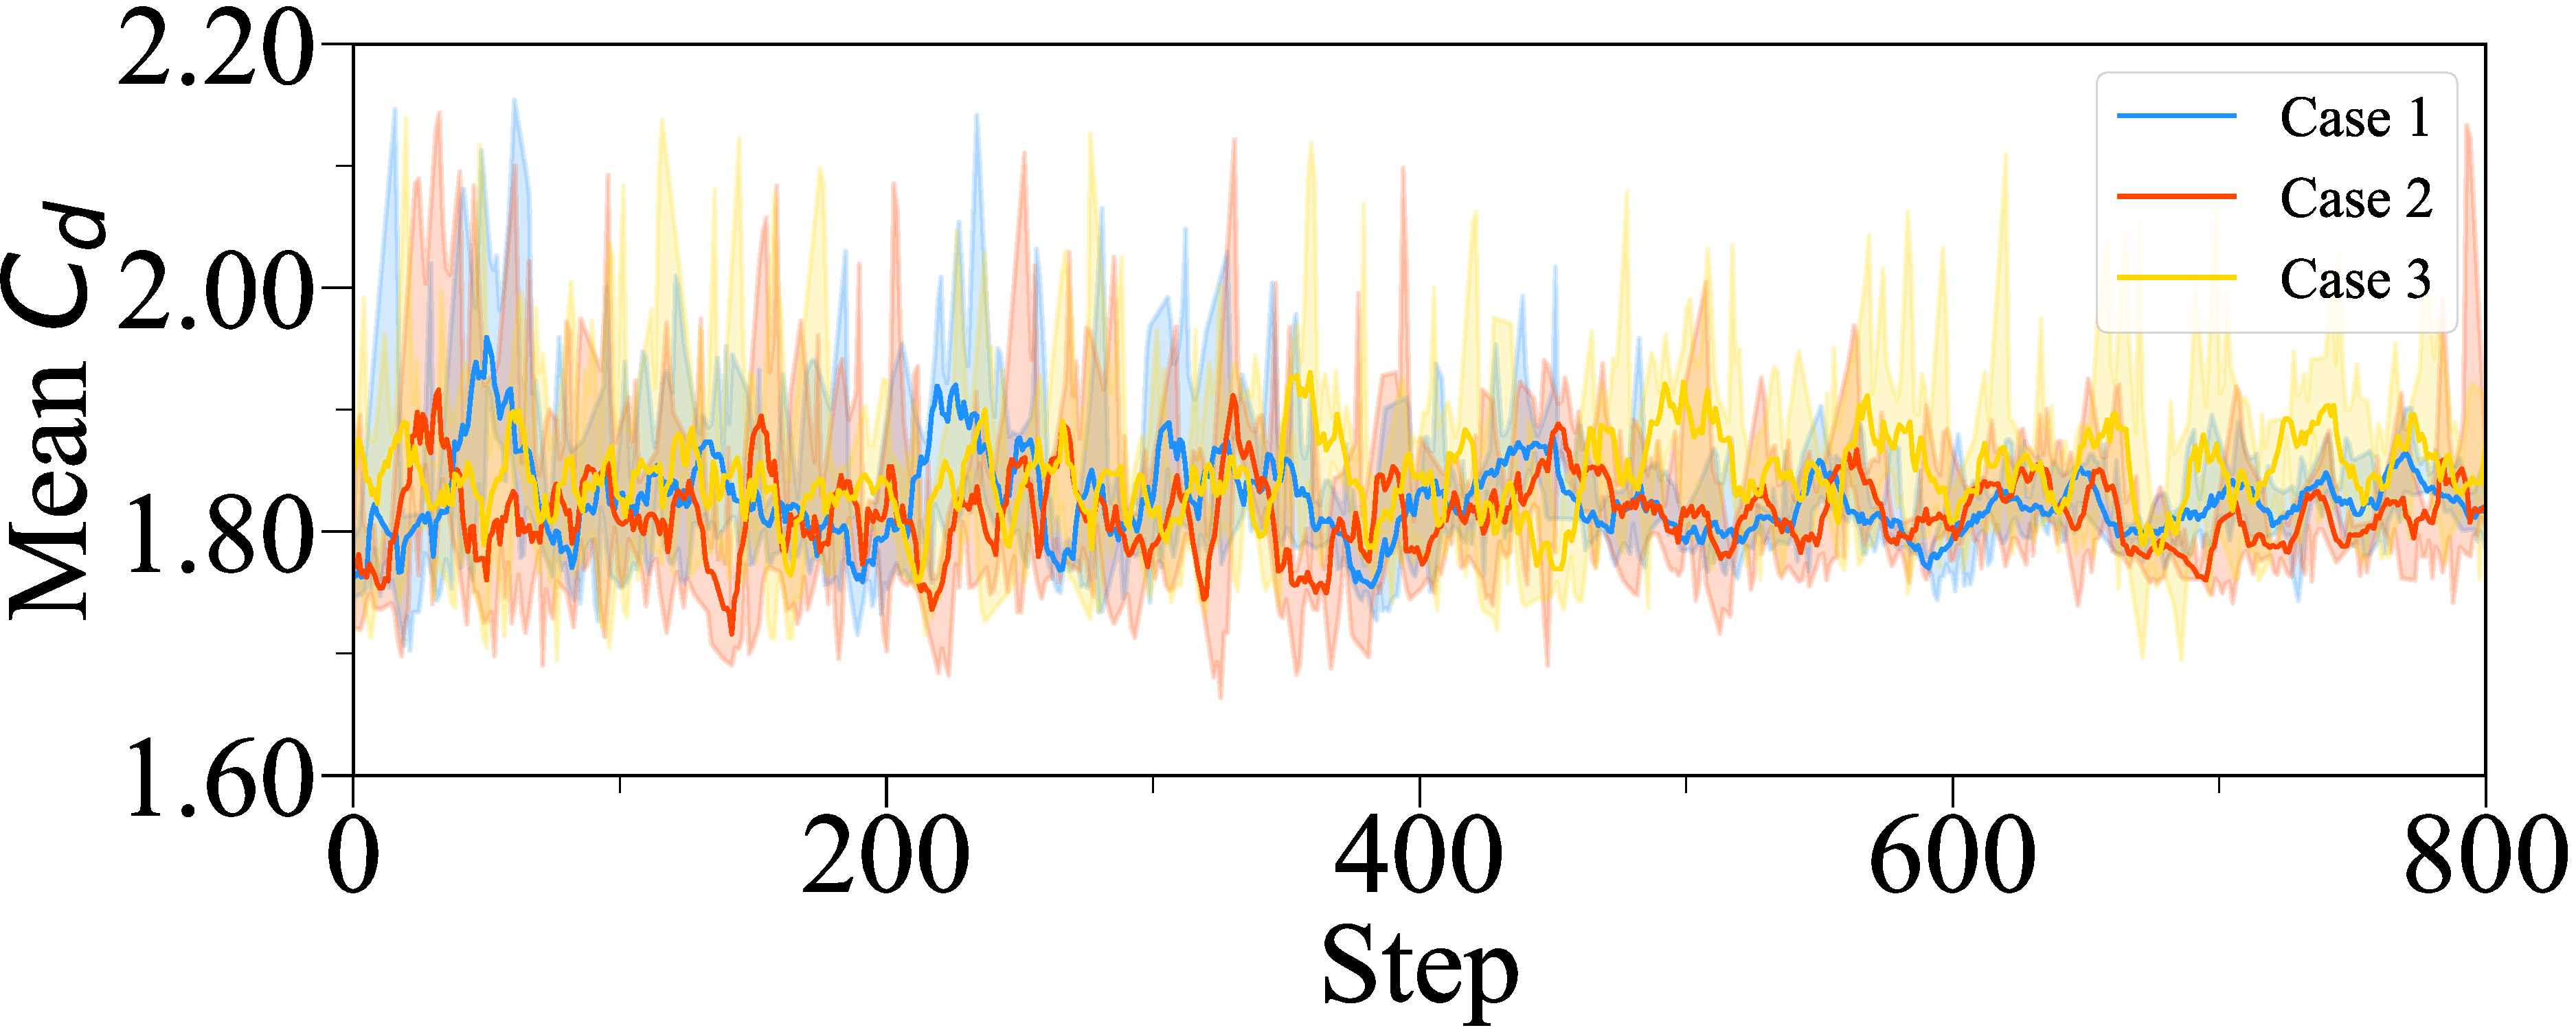
\includegraphics[width=\linewidth]{Cd_1_2_3.pdf}
        \caption{\black{Training curve of Mean $C_d$}}
        \label{Cd_1_2_3}
    \end{subfigure}
    % \hspace{0.5\linewidth}
    \begin{subfigure}{0.9\linewidth} % 第二个子图
        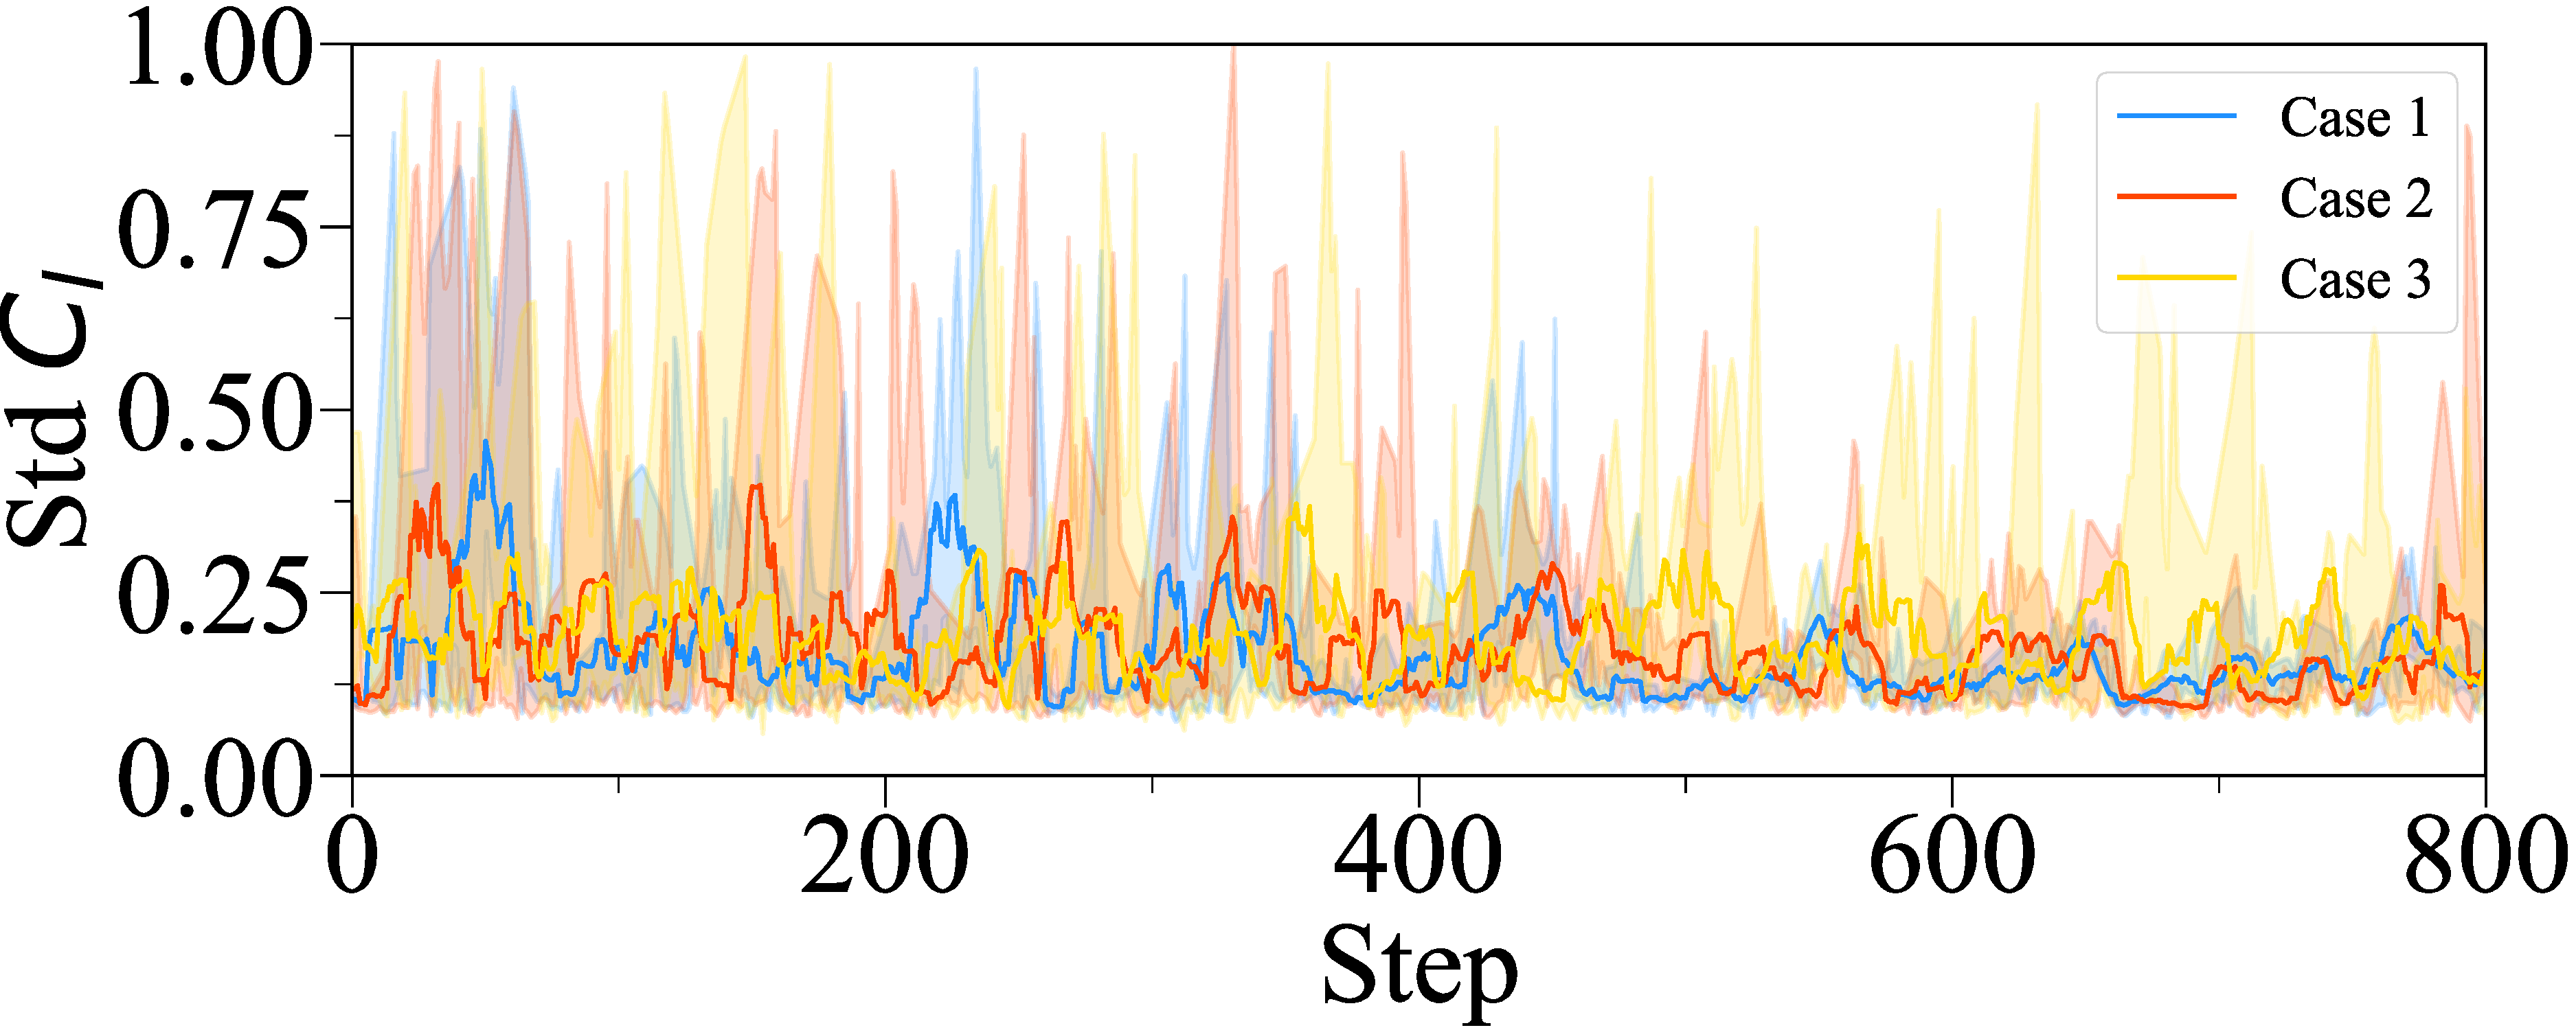
\includegraphics[width=\linewidth]{Cl_1_2_3.pdf}
        \caption{\black{Training curve of Std $C_l$}}
        \label{Cl_1_2_3}
    \end{subfigure}
    
    \caption{Comparison of training curves of reward, mean $C_d$, std $C_l$ in three cases. These curves reveal that the effects of the models from case 1 and case 2 (learning rate = 0.0003) are similar and significantly better than the model from case 3.}
    \label{E123 training}
\end{figure}

\begin{figure*}
    \centering
    
    \begin{subfigure}{1.0\linewidth} % 第一个子图
        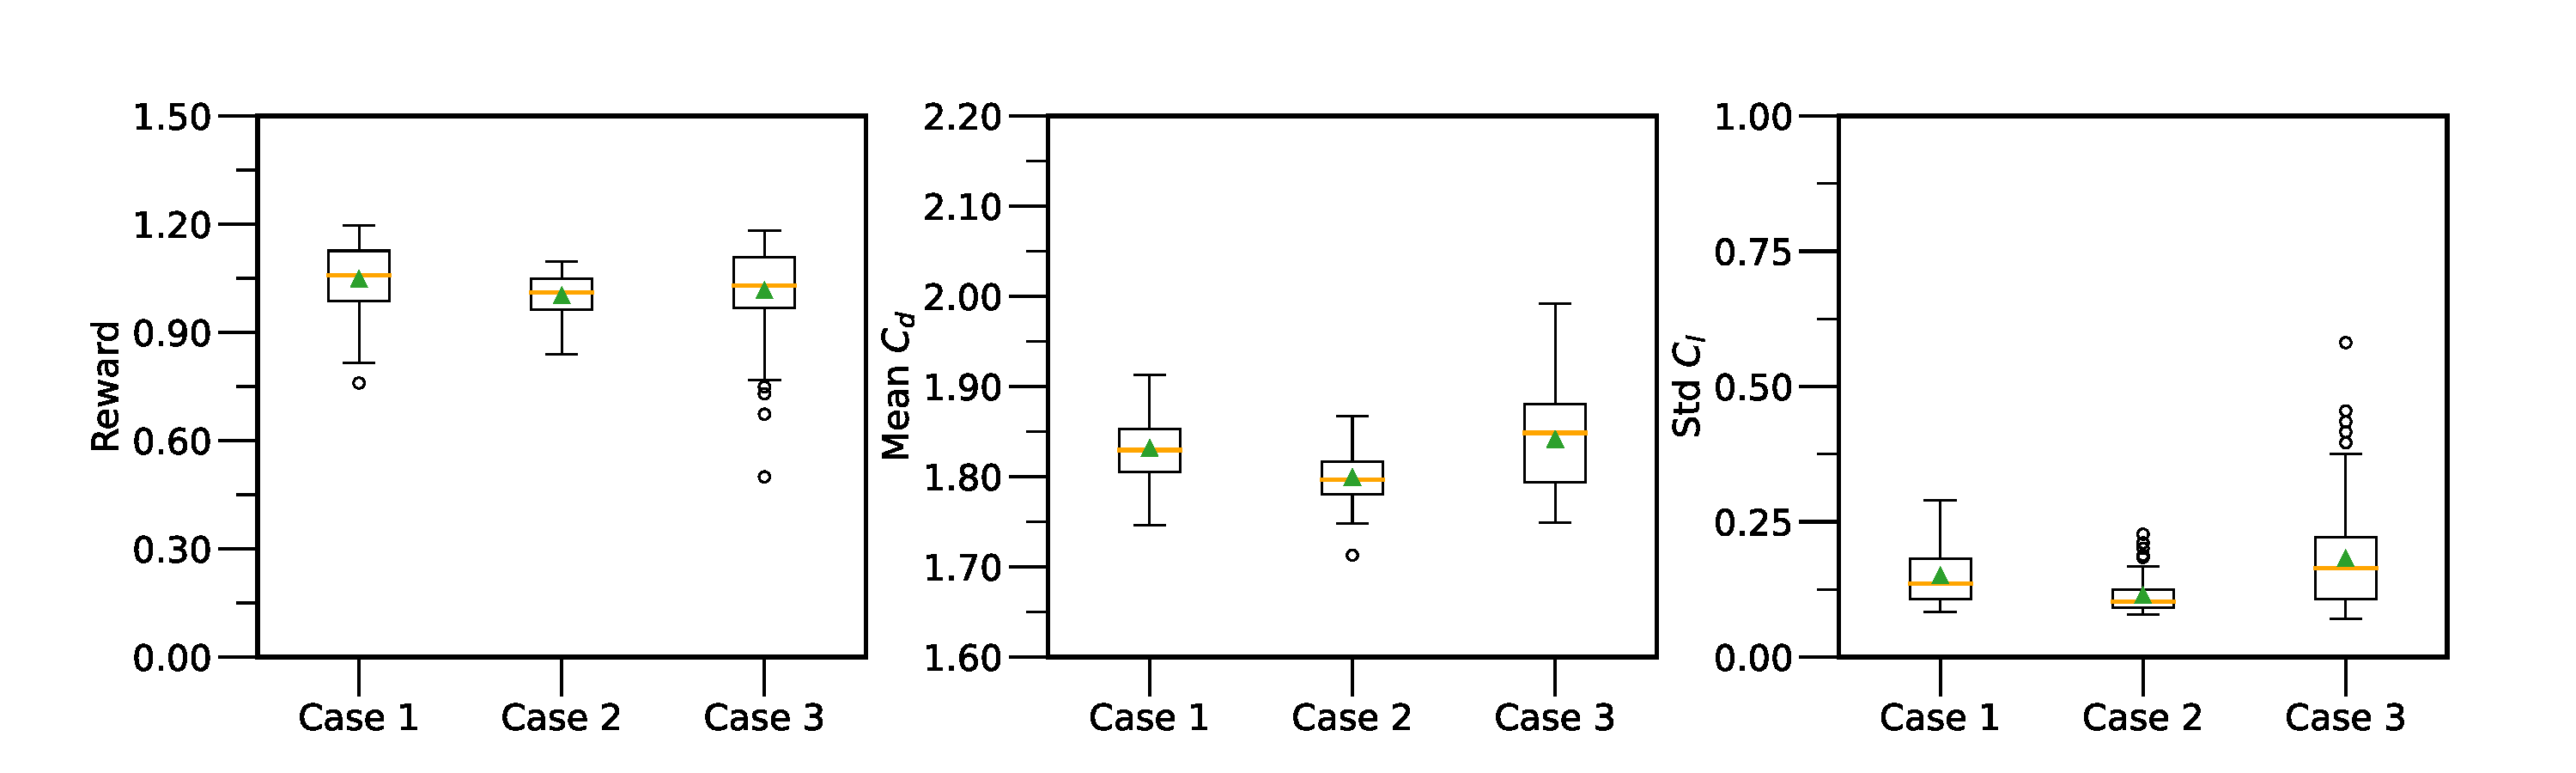
\includegraphics[width=\linewidth]{eval_in_120s_period.pdf}
        \caption{Box plot of reward, mean $C_d$ and std $C_l$ for the models during evaluation in the flow field of case 1.}
        \label{eval_in_120s_period}
    \end{subfigure}
    % \hspace{0.5\linewidth}
    \begin{subfigure}{1.0\linewidth} % 第二个子图
        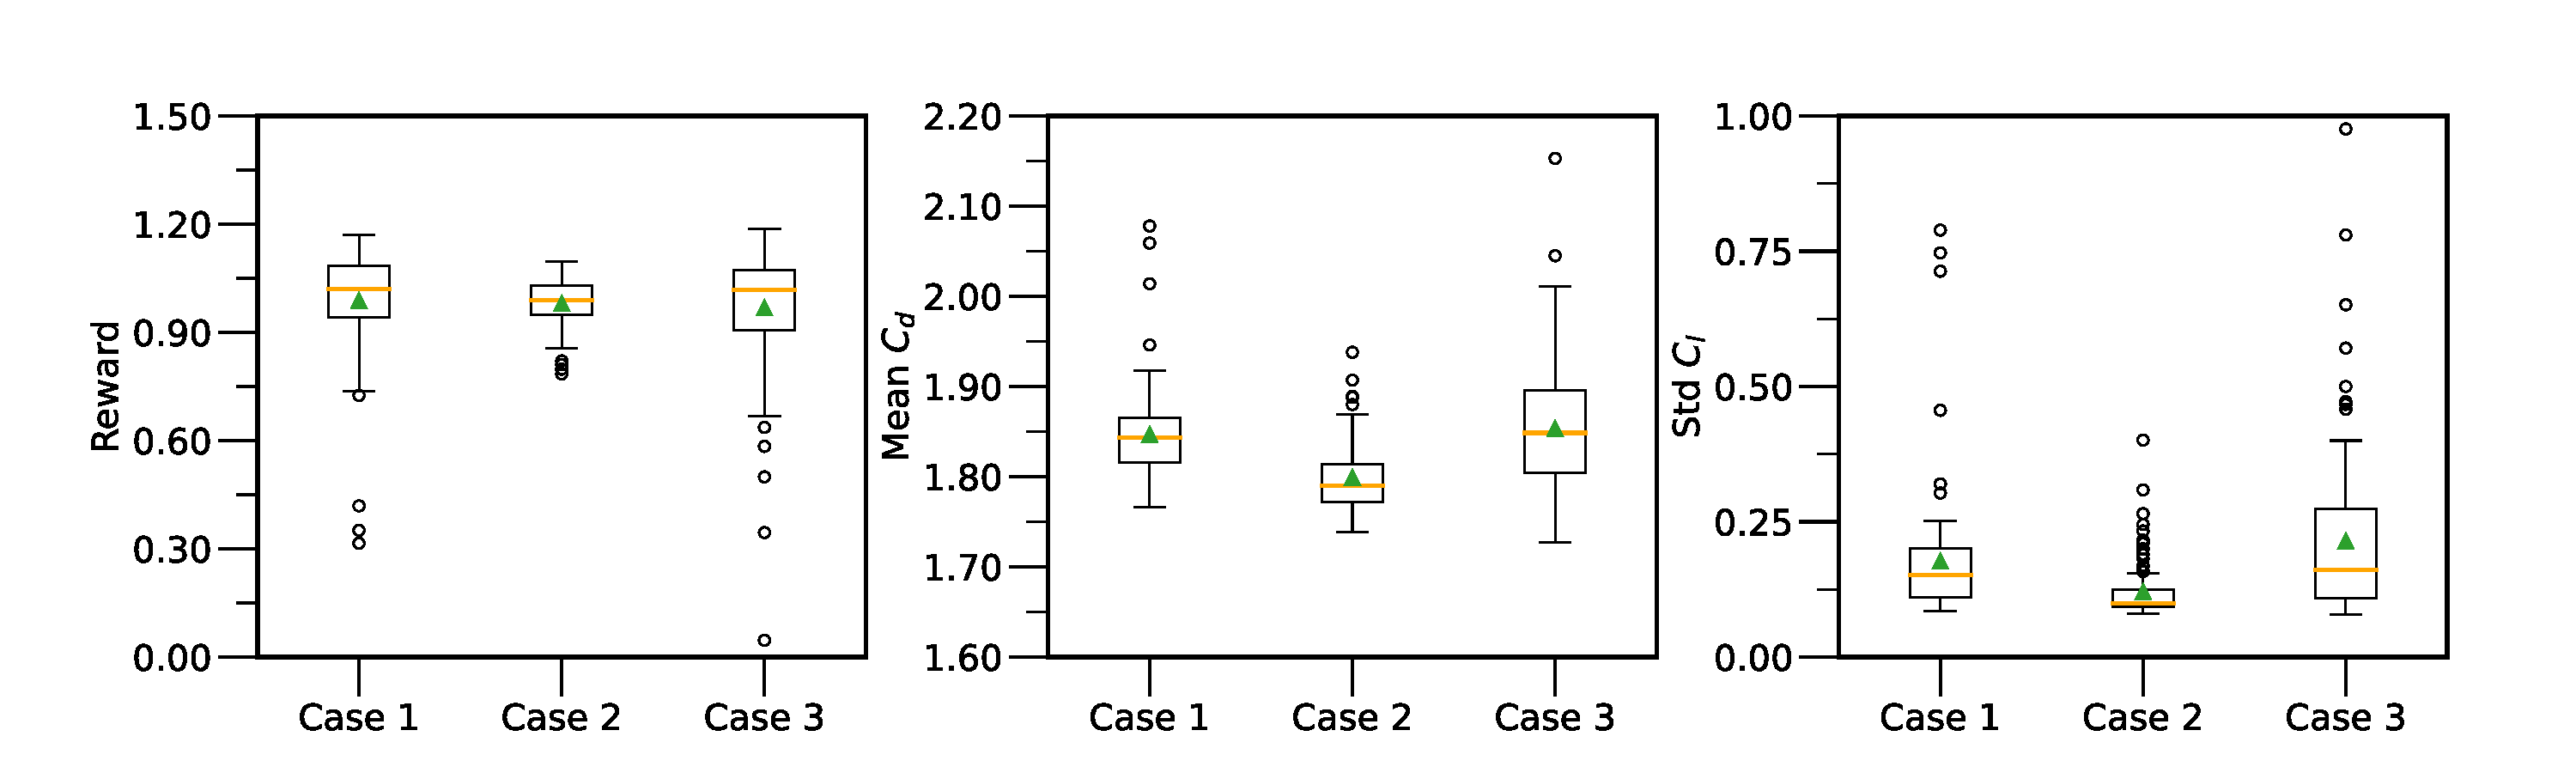
\includegraphics[width=\linewidth]{eval_in_120s_random.pdf}
        \caption{Box plot of reward, mean $C_d$ and std $C_l$ for the models during evaluation in the flow field of case 2.}
        \label{eval_in_120s_random}
    \end{subfigure}
        \begin{subfigure}{1.0\linewidth} % 第二个子图
        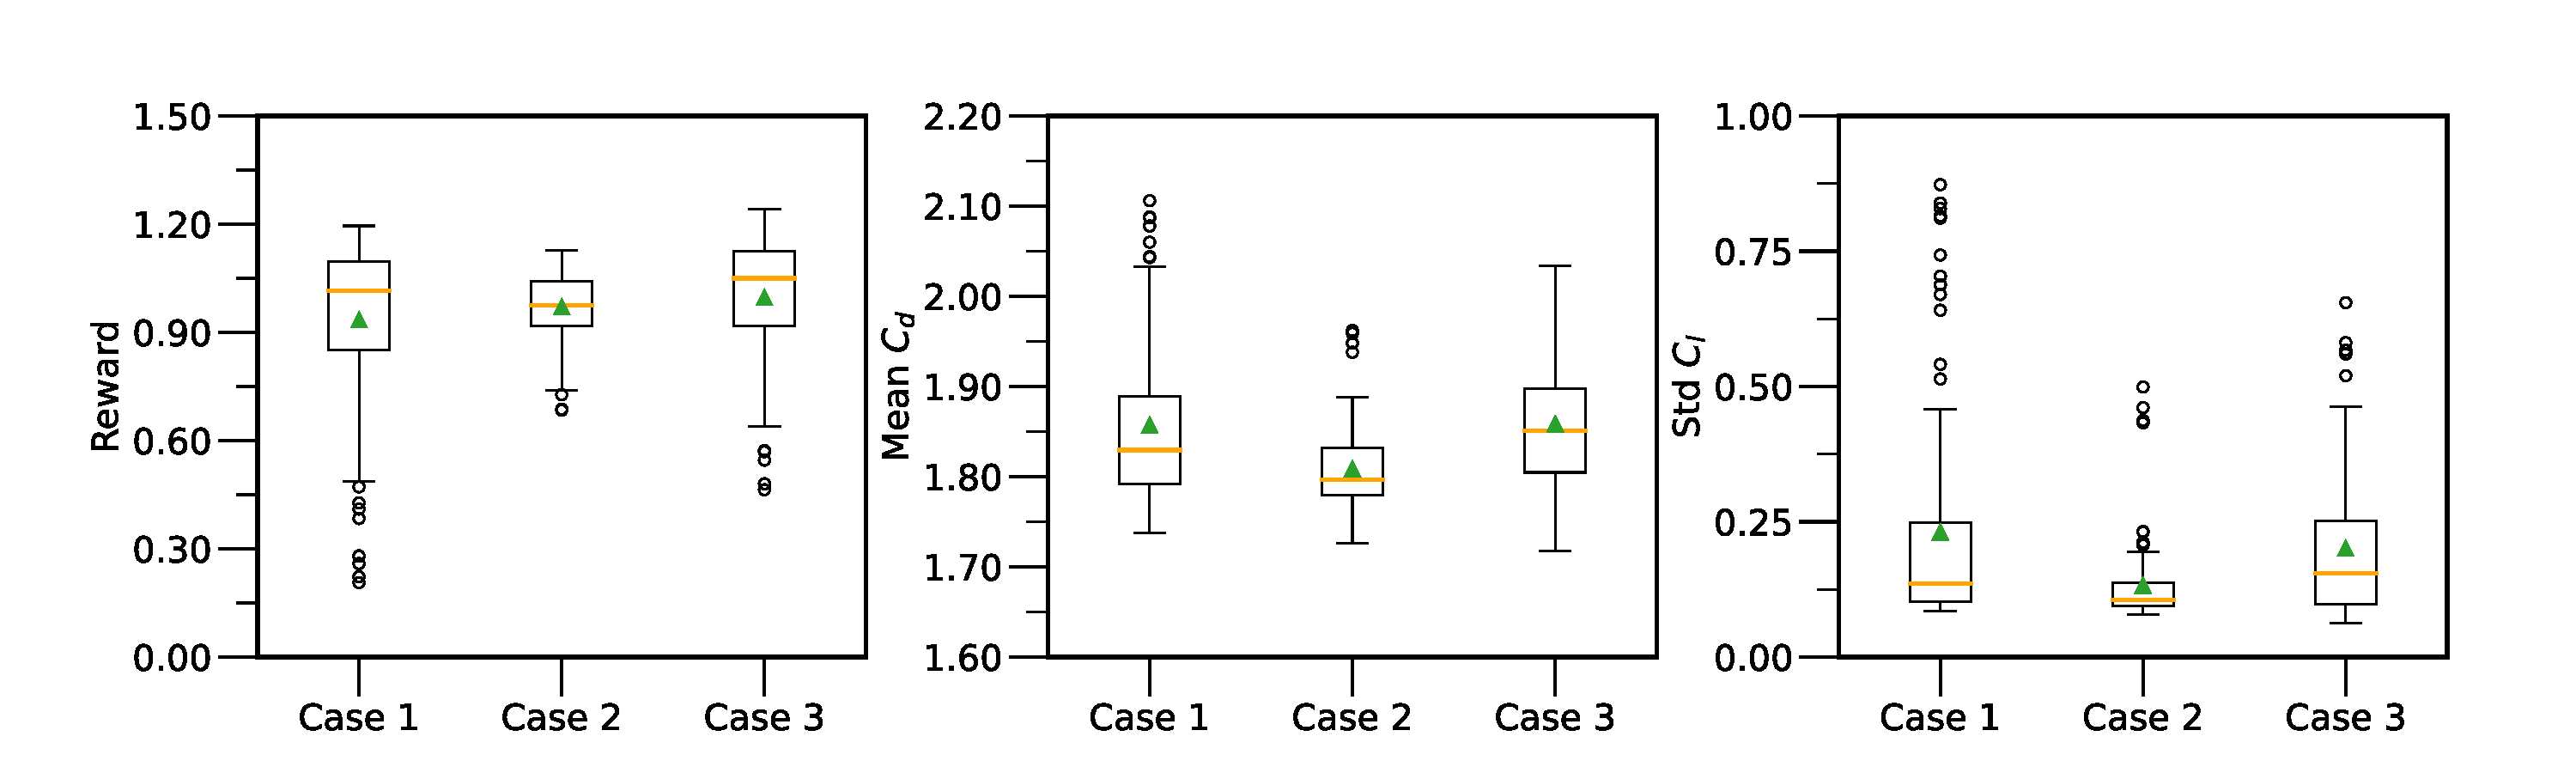
\includegraphics[width=\linewidth]{eval_in_30s.pdf}
        \caption{Box plot of reward, mean $C_d$ and std $C_l$ for the models during evaluation in the flow field of case 3.}
        \label{eval_in_30s_random}
    \end{subfigure}
    
    \caption{Box plots of reward, mean $C_d$, and std $C_l$ for the models from three cases during evaluation.}
    \label{box123}
\end{figure*}

In case 1, the wind velocity in the flow field changed periodically, making environmental changes predictable. However, in the real scenarios, changes in flow field are often more complex and unpredictable. To simulate this complexity, case 2 disrupted the original periodicity and increased the randomness of the flow field, making it a more realistic and challenging scenario.

Case 2 was conducted twice. In the first run, the hyperparameter configuration and adjustments were identical to those in case 1, as shown in Table \ref{hyperparameter in E1}. In the second run, batch size was increased to 512 at step 520, and the learning rate was adjusted to 0.0003. The reward curves for both training processes are displayed in FIG. \ref{reward-2}. It is evident that the reward curve with the mixed learning rate was significantly higher than that with the constant learning rate, indicating an improvement in performance with the adjusted learning rate.

The reason for this was that the training difficulty of case 2 was higher than that of case 1. A smaller learning rate, applied at an appropriate time, could achieve a more refined training effect. As shown in FIG. \ref{Cd-2} and \ref{Cl-2}, mean $C_d$ and std $C_l$ curves stabilized at lower levels, with both curves eventually becoming comparable. Therefore, the difference in reward functions was attributed to the variance in energy consumption. The mixed learning rate could converge to an efficient control strategy while simultaneously reducing the energy consumption associated with control.

Due to the unpredictability of wind velocity, even in the later stages of training, the reward curve still exhibited some large-scale fluctuations. These fluctuations were due to drastic changes in the flow field. The training process often encountered discrepancies between the initially detected wind velocity and the wind velocity when the action was finally realized. Subsequent results indicated that appropriate levels of unpredictability enhanced the adaptability and practicality of the model. 

Based on case 2, case 3 used three values: 0.001, 0.0003, and 0.0001 as the new learning rate at 520 steps. FIG. \ref{E3 training} showed the training curves of reward, $C_d$, and $C_l$ under these three learning rates. The curves that eventually stabilized were similar, without significant differences, and they never achieved a relatively stable state. This is due to the rapid and drastic changes in the flow field, coupled with its unpredictable nature, which make the task more challenging. \black{At this stage, adjusting the learning rate does not lead to noticeable performance improvements.}

Consequently, the results of the three cases were compared, using a mixed learning rate of 0.0003 in case 2 and a mixed learning rate of 0.0001 in case 3. The comparison results were shown in FIG. \ref{E123 training}. The curves indicated that the training results in case 1 and case 2 were similar and both were significantly better than those in case 3. This suggests that the training difficulty increases as the complexity of the flow field grows, highlighting the challenge of achieving optimal control in more dynamic and unpredictable environments.

\subsection{\black{Evaluation and validation of DRL models}}

\begin{figure}
    \centering

    \begin{subfigure}{0.8\linewidth} % 第一个子图
        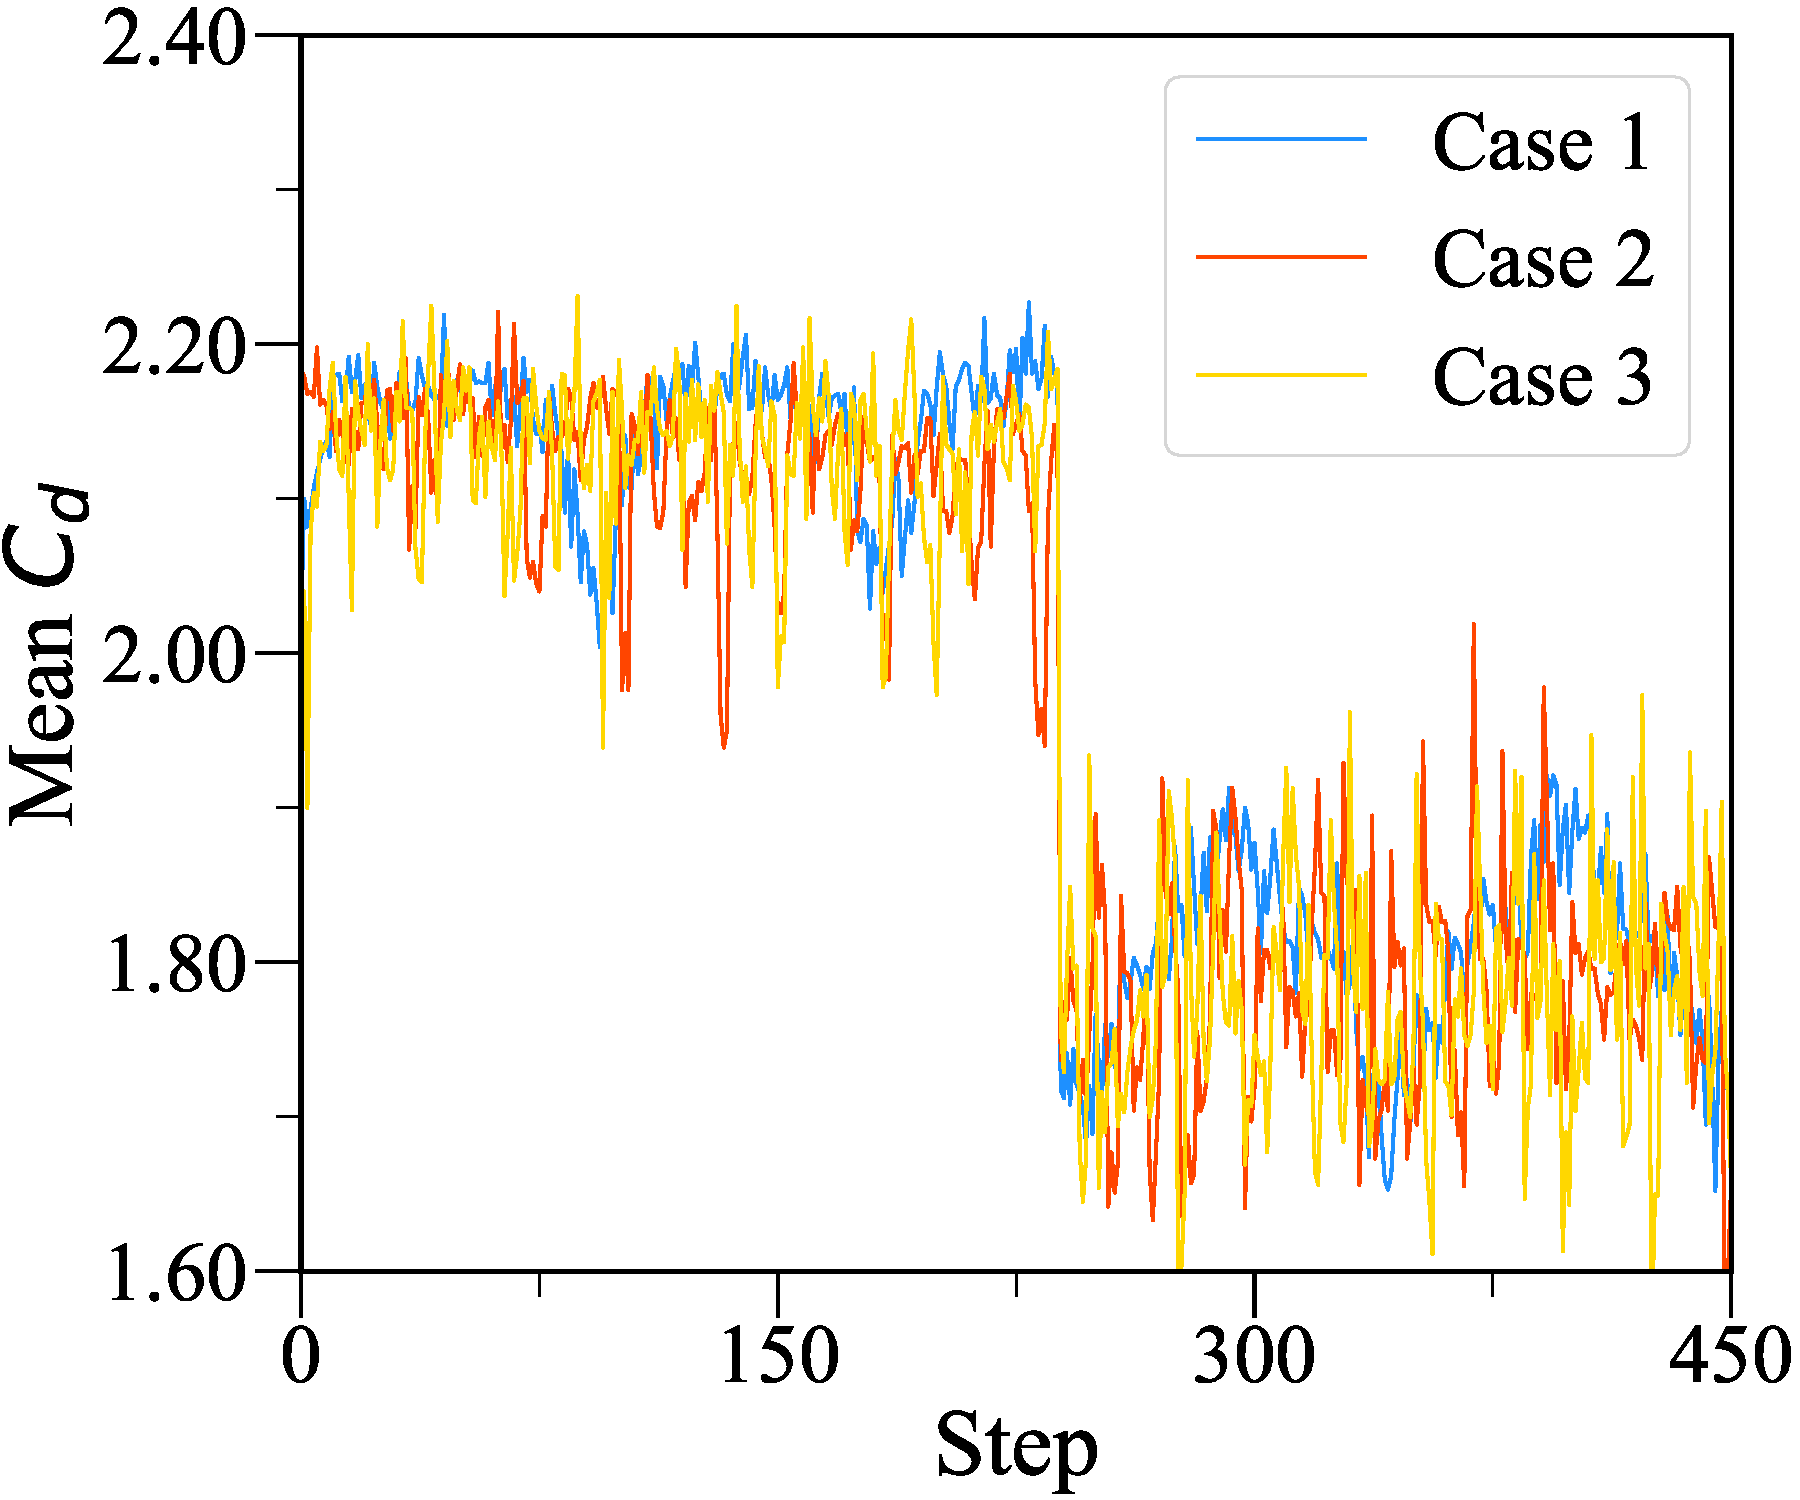
\includegraphics[width=\linewidth]{Cd_test.pdf}
        \caption{Mean $C_d$ curve}
        \label{final cl}
    \end{subfigure}
    \begin{subfigure}{0.8\linewidth} % 第一个子图
        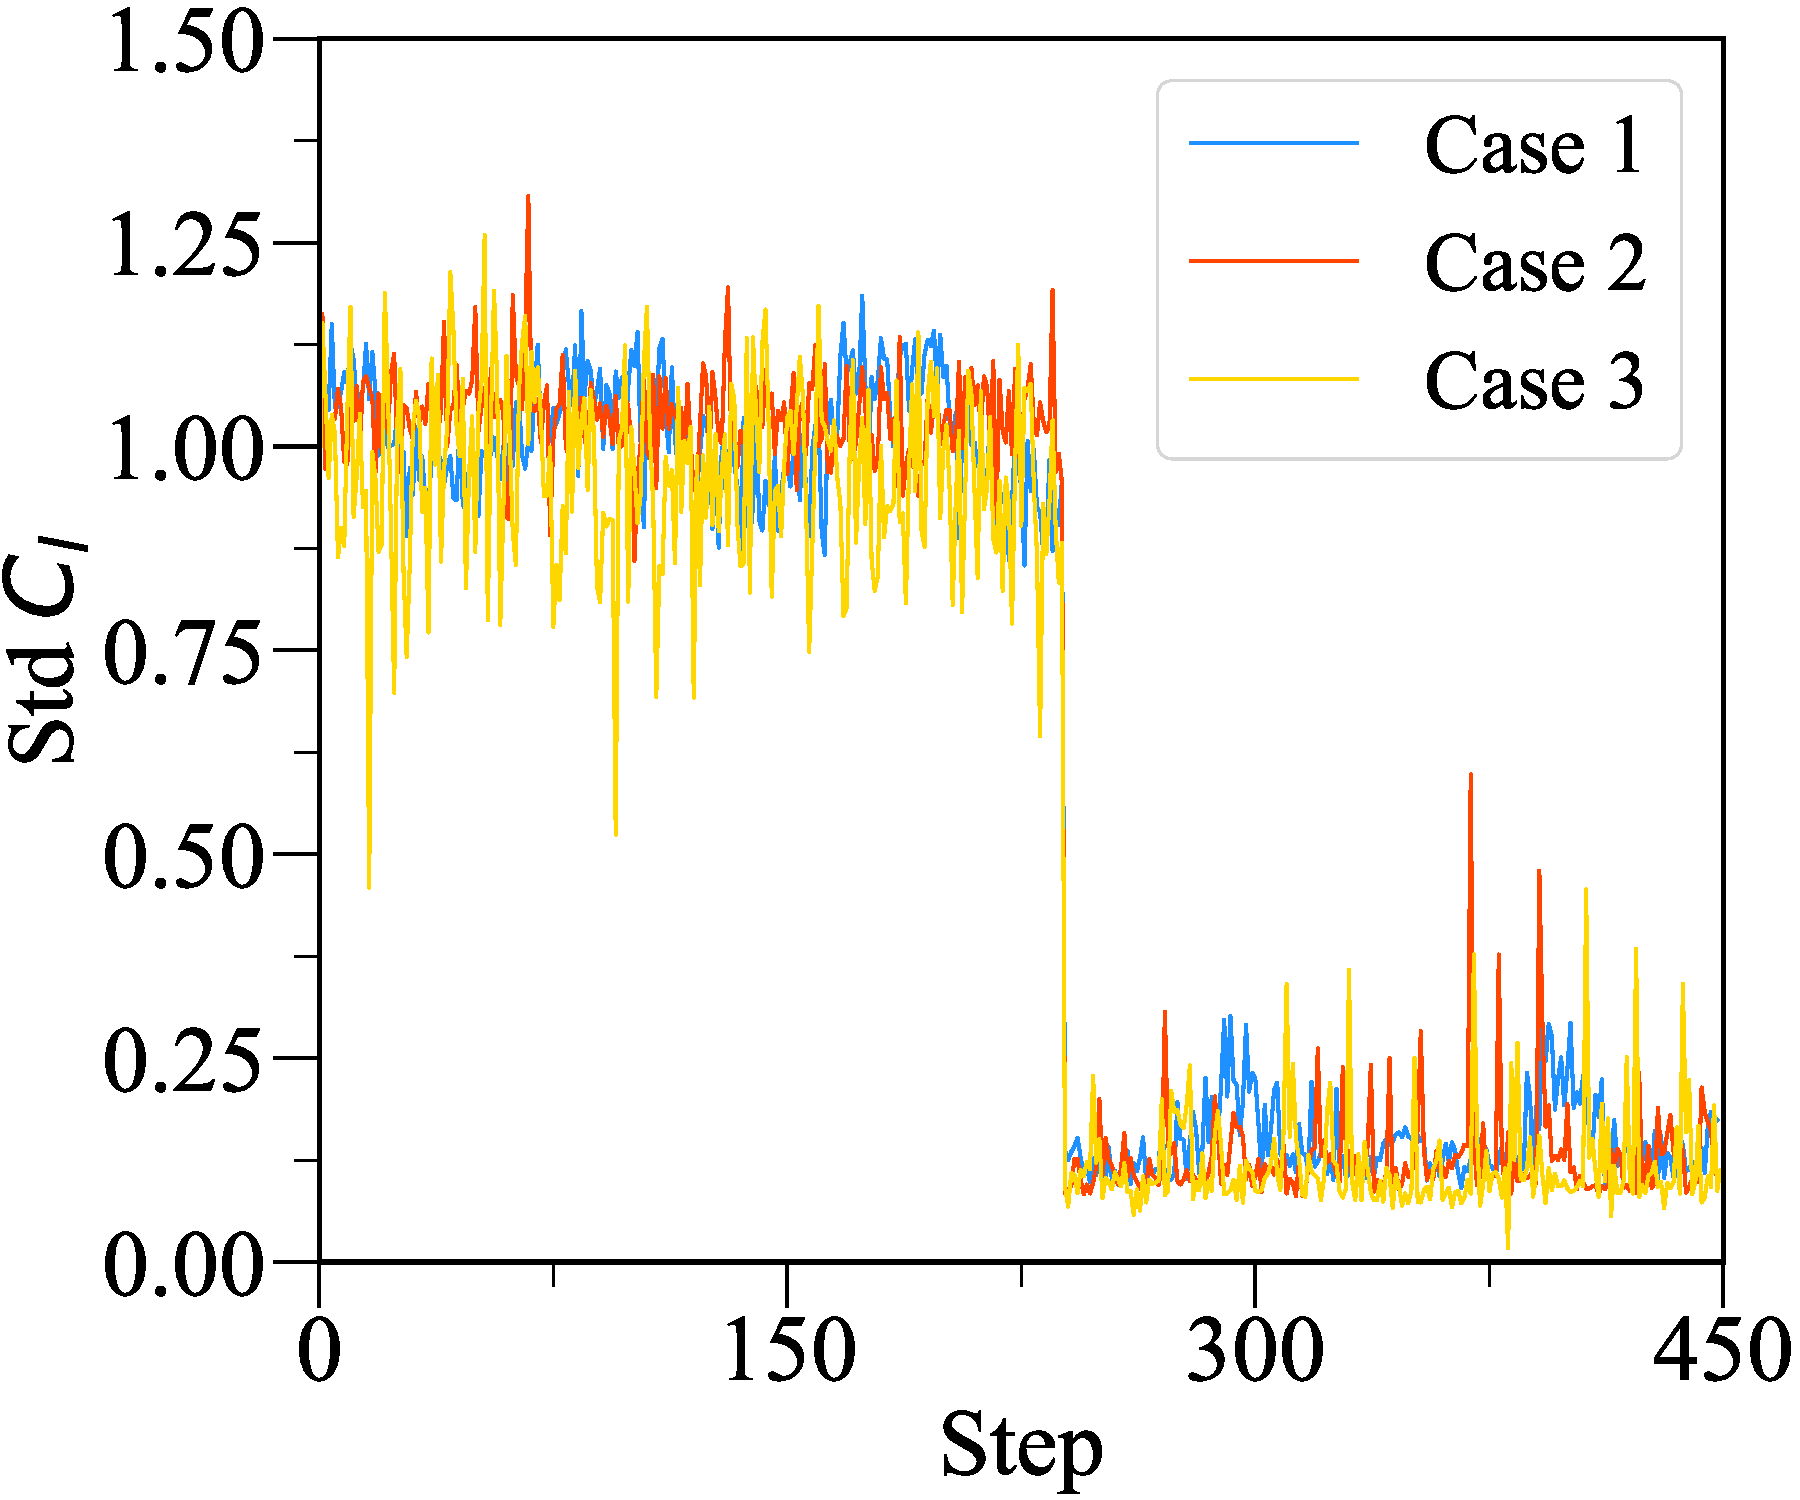
\includegraphics[width=\linewidth]{Cl_test.pdf}
        \caption{Std $C_l$ curve}
        \label{final cd}
    \end{subfigure}

    
    \caption{\black{Validation} for the most robust model (from case 2) in the flow fields of three cases, with control initiated at step 240.}
    \label{final training}
\end{figure}

\begin{figure}[htb]
\centerline{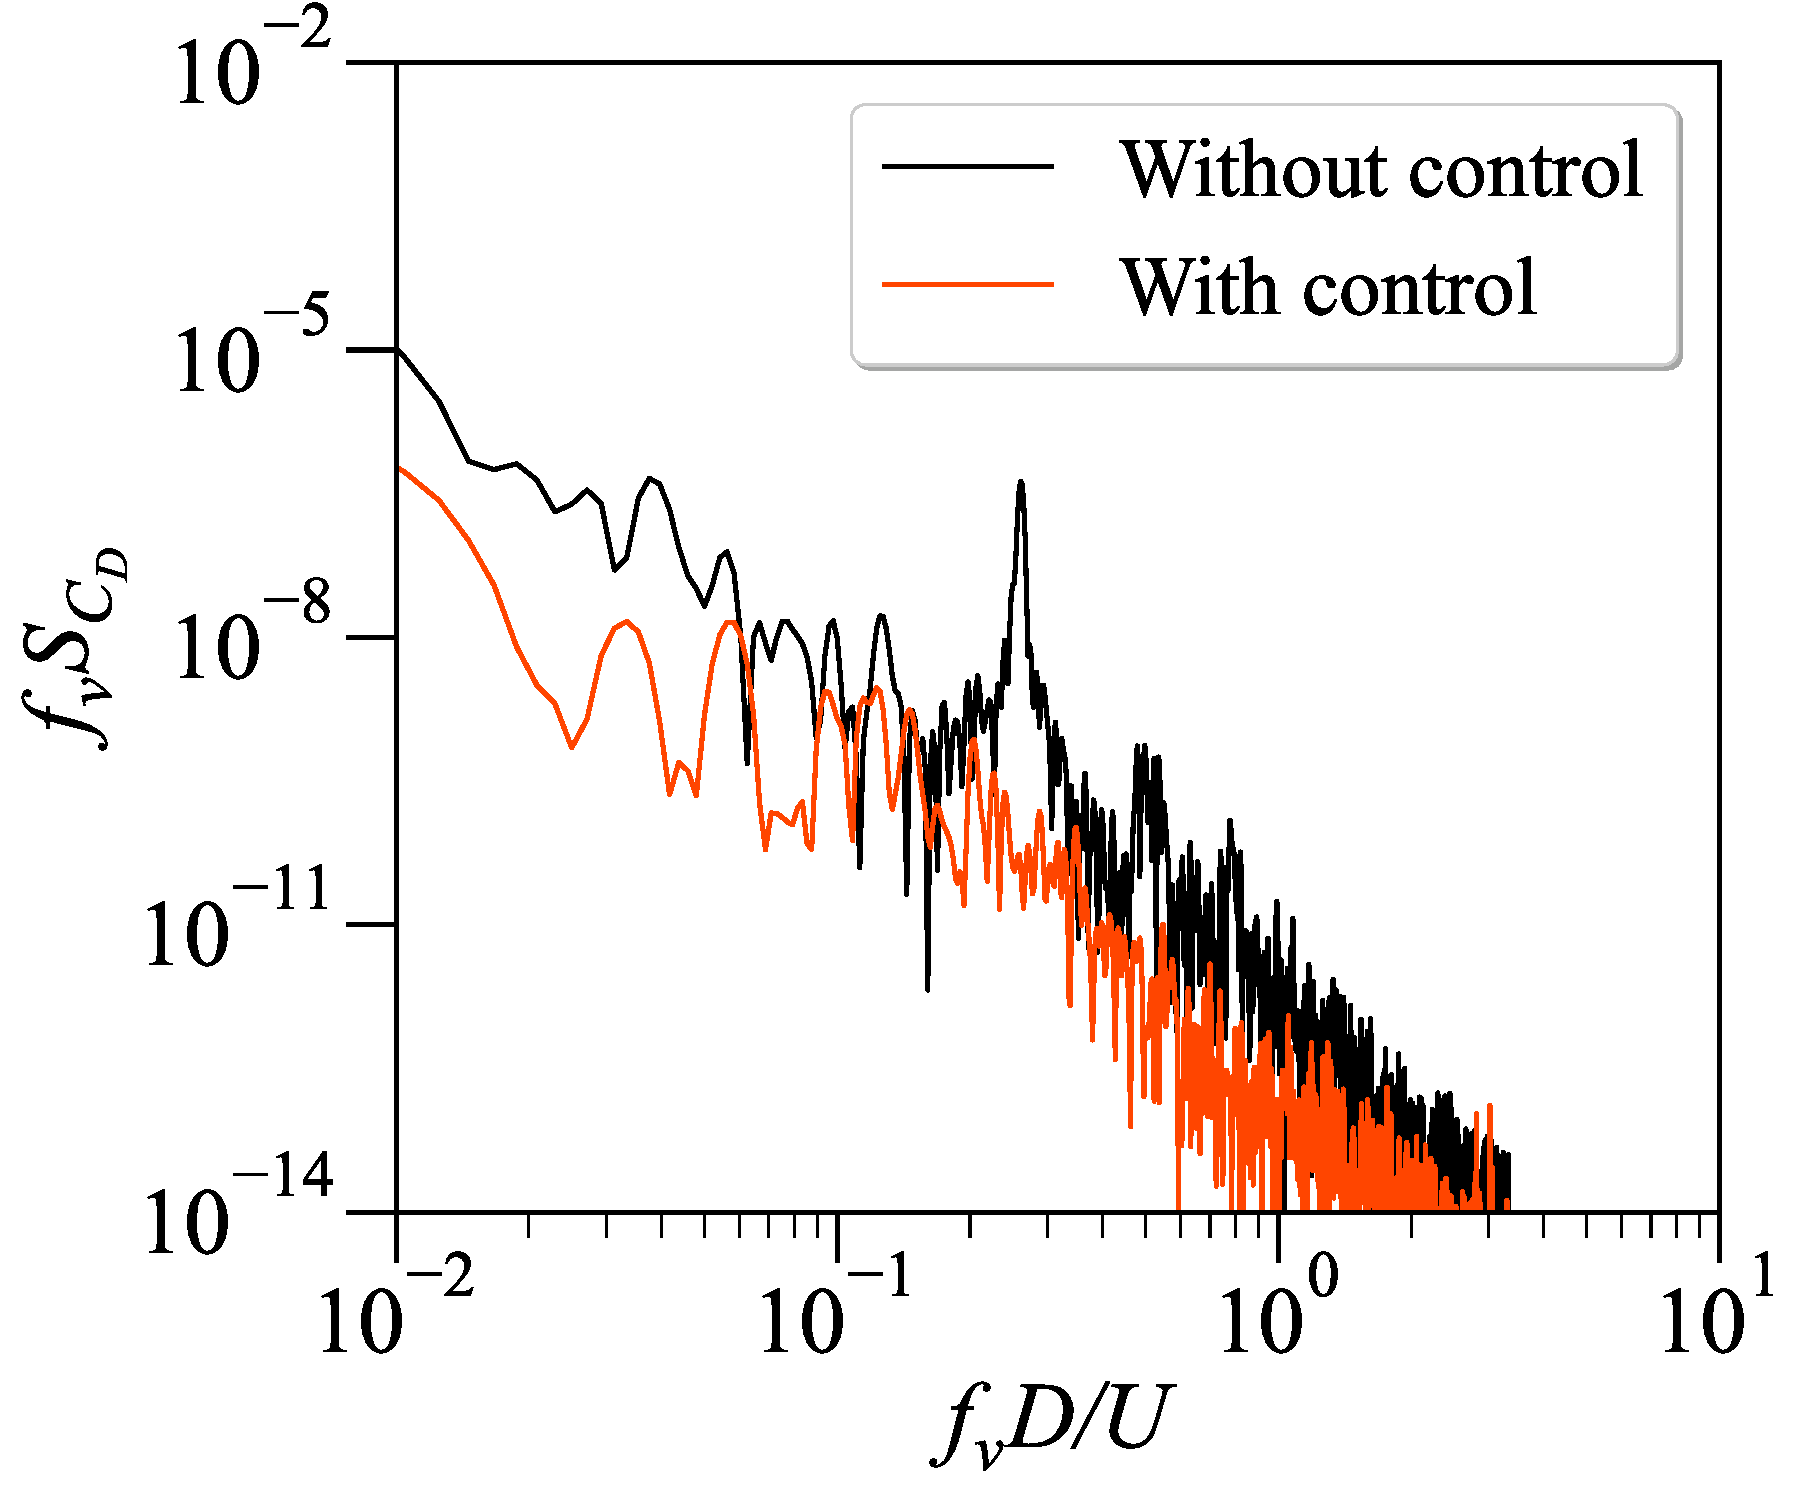
\includegraphics[width=0.8\linewidth]{result.pdf}}
\caption{\black{Power spectral density curves with and without control at a wind velocity of 5.8 m/s}}
\label{fft}
\end{figure}



\begin{figure}
    \centering

    \begin{subfigure}{0.8\linewidth} % 第一个子图
        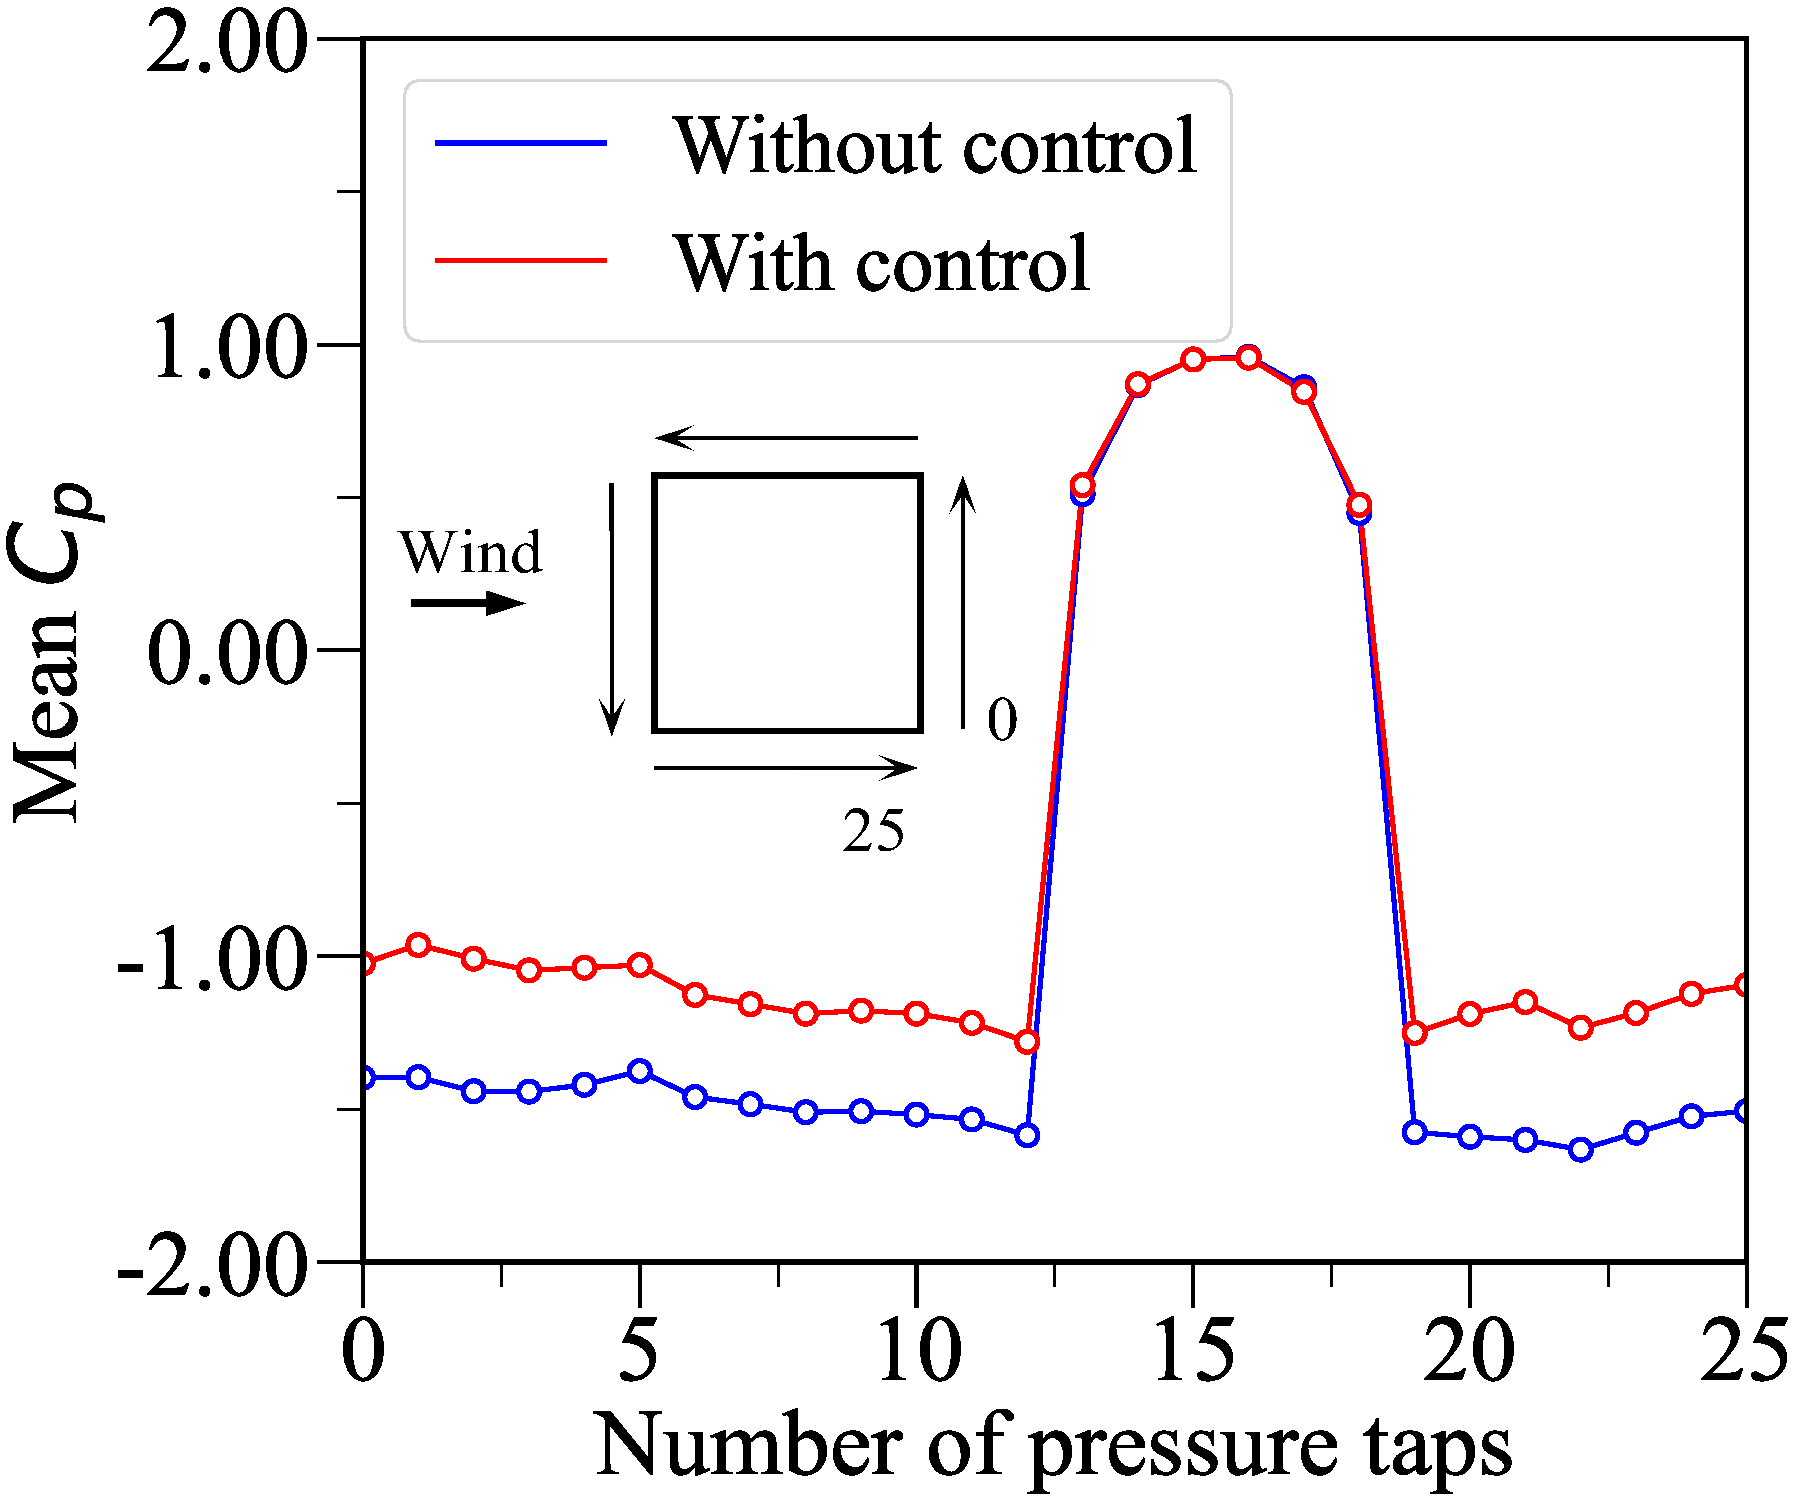
\includegraphics[width=\linewidth]{Cp_mean.pdf}
        \caption{Mean of pressure coefficient $C_p$}
        \label{Cp-mean}
    \end{subfigure}
    \begin{subfigure}{0.8\linewidth} % 第一个子图
        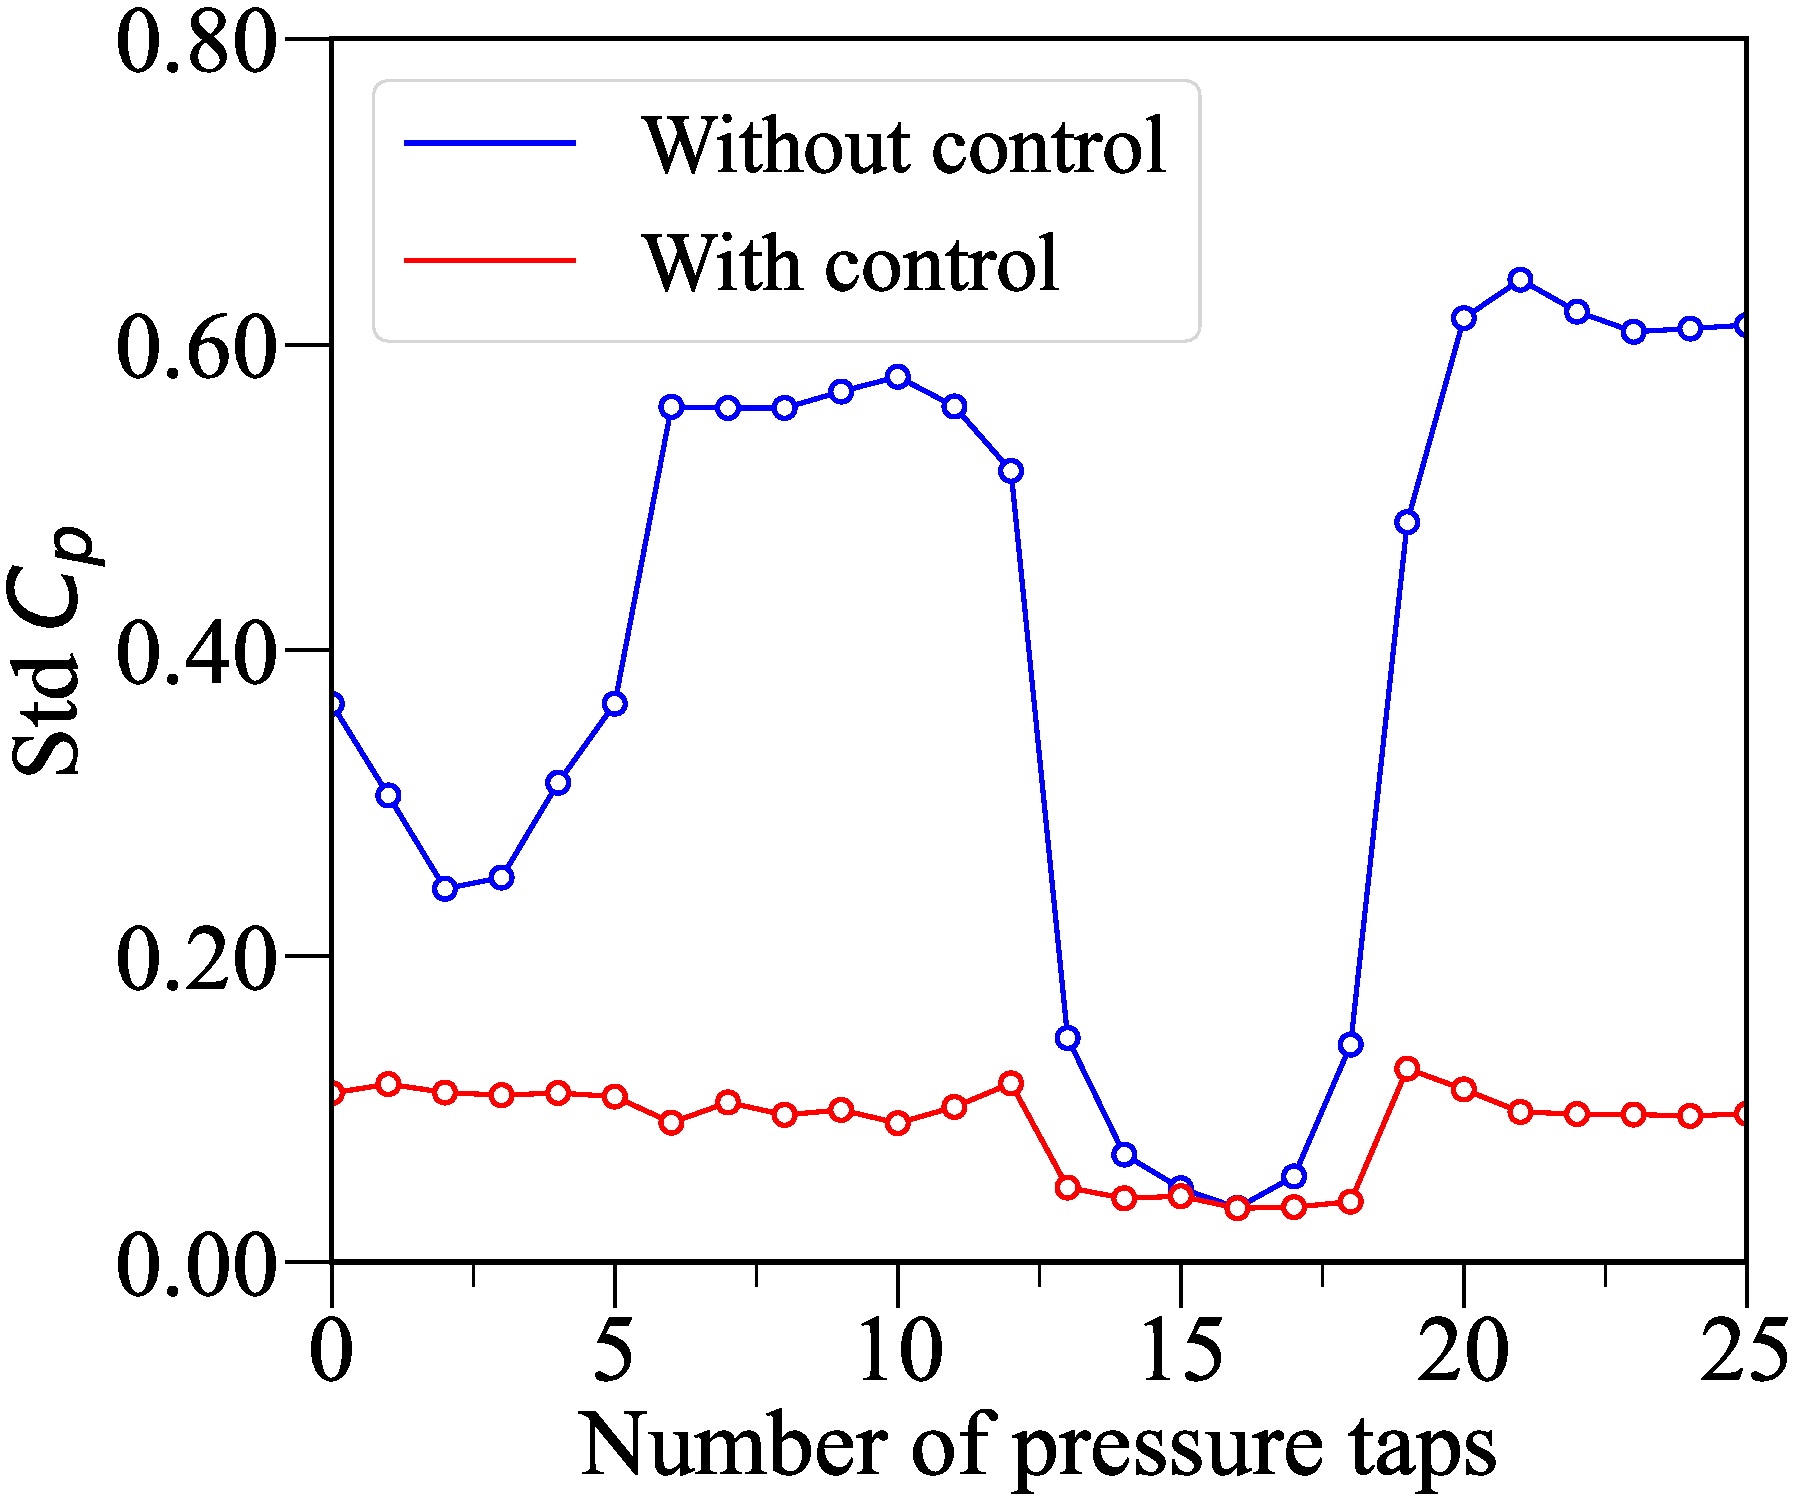
\includegraphics[width=\linewidth]{Cp_std.pdf}
        \caption{Std of pressure coefficient $C_p$}
        \label{Cp-std}
    \end{subfigure}
    
    \caption{\black{Mean and standard deviation of pressure coefficient along surface of square cylinder at an incoming wind velocity of 5.8 m/s}}
    \label{Cp}
\end{figure}

To compare the advantages and disadvantages of the models obtained from the three cases, the optimal models from each case were tested and compared under the flow fields of the three respective cases. The results are displayed as box plots in FIG. \ref{box123}. \black{FIG. \ref{eval_in_120s_period}, \ref{eval_in_120s_random} and \ref{eval_in_30s_random} represent reward, mean $C_d$ and std $C_l$ obtained from evaluating the models in the wind fields of three cases.}

In these box plots, the upper and lower edges of the boxes represent the upper and lower quartiles respectively. The median is indicated by the central orange line, while the highest and lowest horizontal lines denote the maximum and minimum values within the data set. Outliers are marked with circles, and mean value is shown as a green triangle. The height of the box and the extent of outlier deviation are directly proportional to the degree of performance fluctuation in the models. Meanwhile, mean value and median offer insights into the overall performance of the models, providing an understanding of how the models perform with and without the influence of outlier samples. 

From the figure, it can be observed that the average and median reward of the three models across the three flow fields are relatively consistent; however, there are notable differences in the stability. The model from case 2 demonstrates the highest stability across all three flow fields. In contrast, the model from case 1 exhibits good stability within its own training flow field but performs poorly in the other two flow fields. The model from case 3, on the other hand, shows poor stability across all three flow fields.

In terms of drag and lift coefficients, the performance of the three models varies significantly, further highlighting the differences in their adaptability and performance across different flow conditions.

\black{In FIG. \ref{eval_in_120s_period}, for mean $C_d$ and std $C_l$, the model from case 2 demonstrates the best mean and median, followed by case 1, with case 3 being the worst. In terms of stability, the models rank in the order of case 1 > case 2 > case 3.}

\black{In FIG. \ref{eval_in_120s_random}, for mean $C_d$ and std $C_l$, mean and median rankings of the three models are: case 2 < case 1 $\le$ case 3. In terms of stability, the models rank as case 2 > case 1 $\ge$ case 3.}

\black{In FIG. \ref{eval_in_30s_random}}, for mean $C_d$, the performance order is consistent with the first two flow fields, with mean and median values ranked as case 2 < case 1 $\le$ case 3. Besides, the stability order is case 2 > case 3 $\ge$ case 1. For std $C_l$, the model from case 2 performs the best in terms of median, mean, and stability, followed by case 3, with case 1 performing the worst.

In summary, the most robust model among the three originates from case 2. Except for the reward and mean $C_d$ in the flow field of case 1, where it is slightly inferior to the model from case 1, the model from case 2 performs the best in nearly all scenarios across the three flow fields. In the other two flow fields, its performance significantly surpasses that of the other two models.

Subsequently, the model obtained in case 2 was subjected to \black{validation}. The test method is as follows: First, the wind field is initiated, and the blowing pipes are closed. Data for mean $C_d$ and std $C_l$ are recorded without control. At the 240th step, the blowing pipes are opened and controlled using the DRL model from case 2. The result curves of mean $C_d$ and std $C_l$ during the test are shown in FIG. \ref{final training}.

From the figures, the DRL model from case 2 can effectively reduce drag and lift coefficients of the two-dimensional square cylinder under three different flow fields, with mean $C_d$ reduced by approximately 16\% and std $C_l$ reduced by about 88\%. This not only demonstrates the ability of DRL but also verifies the effectiveness of DRLinWT in facilitating communication between DRL and wind tunnel testing.

\subsection{\black{Spectrum and surface pressure coefficient analysis}}

\black{A pair of lift data for the controlled and uncontrolled two-dimensional square cylinder at a consistent wind velocity of 5.8 m/s was randomly selected from the validation of DRL model of case 2 for spectrum and pressure coefficient analysis.}

\black{\textbf{Spectrum Analysis.} The frequency was converted into the Strouhal number, with the results shown in FIG. \ref{fft}. As illustrated, following the application of blowing control, the primary peak associated with vortex shedding is no longer present. This outcome indicates that the control strategy effectively suppresses vortex shedding energy, thereby reducing the aerodynamic fluctuations acting on the square cylinder.}

\black{\textbf{Pressure Coefficient Analysis.} Pressure coefficient analysis was conducted using data from pressure taps on the row without blowing holes, as shown in FIG. \ref{pressuretaps}. FIG. \ref{Cp} presents mean and standard deviation of the pressure coefficient distribution along surface of the model.}

\black{As shown in FIG. \ref{Cp-mean}, the pressure coefficient on the windward of the model remains nearly unchanged after control, while mean pressure coefficients on the other three sides are reduced. Notably, the negative pressure on the leeward incrases, aligning with the observed reduction in mean $C_d$ in the validation. In FIG. \ref{Cp-std}, it can be seen that following blowing control, the standard deviation of the pressure coefficients on both sides is significantly reduced, consistent with the substantial reduction in std $C_l$ observed in the validation.}





\begin{figure*}
    \centering
    
    \begin{subfigure}{0.3\linewidth} % 第一个子图
        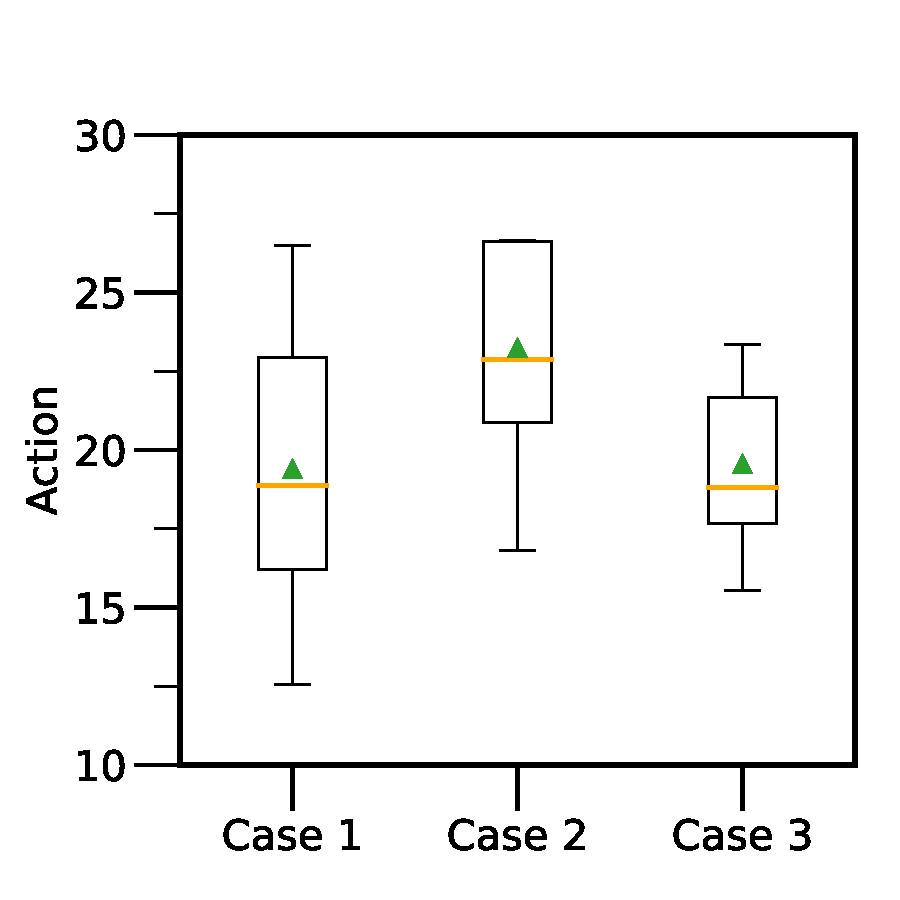
\includegraphics[width=\linewidth]{eval_action_box_2mins_period_env.pdf}
        \caption{Action box plot for the models during evaluation in the flow field of case 1.}
        \label{action_in_120s_period}
    \end{subfigure}
    % \hspace{0.5\linewidth}
    \begin{subfigure}{0.3\linewidth} % 第二个子图
        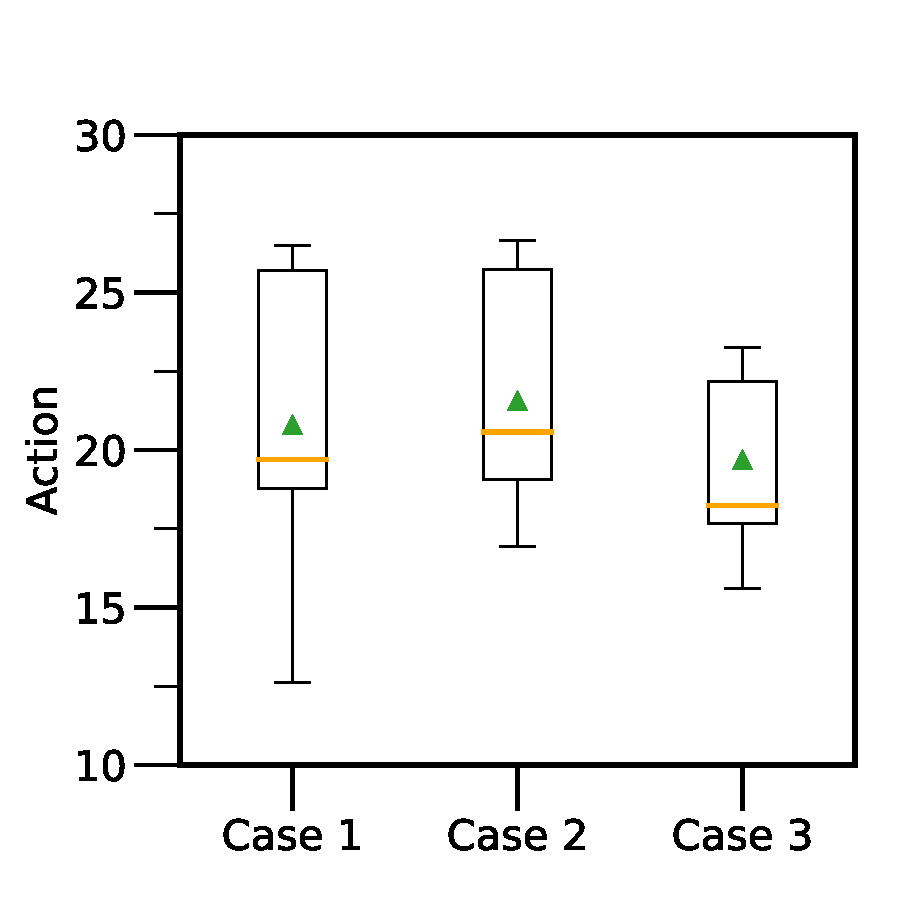
\includegraphics[width=\linewidth]{eval_action_box_2mins_random_env.pdf}
        \caption{Action box plot for the models during evaluation in the flow field of case 2.}
        \label{action_in_120s_random}
    \end{subfigure}
        \begin{subfigure}{0.3\linewidth} % 第二个子图
        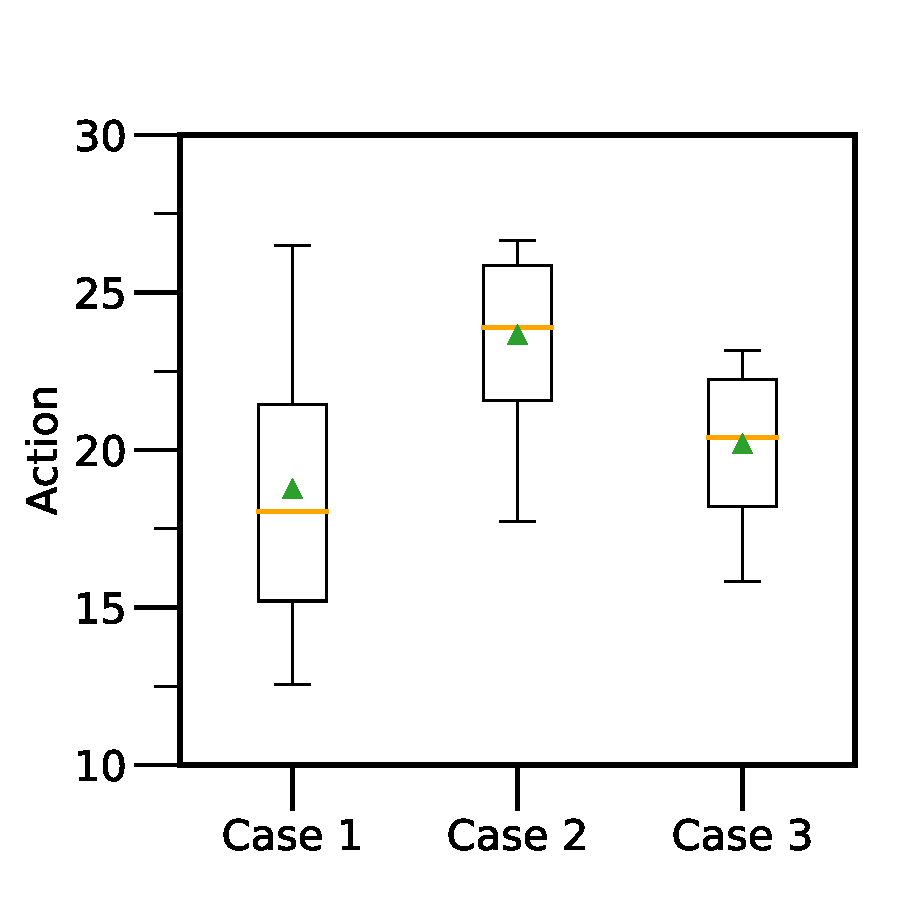
\includegraphics[width=\linewidth]{eval_action_box_30s_random_env.pdf}
        \caption{Action box plot for the models during evaluation in the flow field of case 3.}
        \label{action_in_30s_random}
    \end{subfigure}
    
    \caption{Action box plots for the models from three cases during evaluation.}
    \label{box_action}
\end{figure*}

\subsection{Discussions}

The reason for this phenomenon can be analyzed from the action box plots of the three models. As shown in FIG. \ref{box_action}, \black{the action box plots for the three models during evaluation in the different flow fields reveal distinct patterns. The action values of the model from case 1 are widely distributed, ranging from $13 \sim 27$ L/min. In contrast, the model from case 2 shows a more concentrated range, with higher flow rates between $18 \sim 26$ L/min, while the model from case 3 is focused on moderate flow rates, around $16 \sim 23$ L/min.}

In the flow field of case 1, the environment is predictable, and the agent does not encounter low reward caused by unexpected wind velocity variations. As a result, the optimal flow rate at each step is well-defined, allowing the model to effectively manage varying wind velocities and a broad range of actions. Furthermore, due to the gradual changes in wind velocity, the model can consistently select the actions that yield the highest reward at each step, thereby maximizing the cumulative reward. However, when applied to unpredictable environments, the model struggles to adapt to abrupt and irregular wind velocity changes, leading to a significant decline in performance.

In contrast, the model from case 3, trained in a more complex and variable flow field, faces significant challenges. The fluctuating wind velocities strain the model, as it must frequently manage situations where the flow rate is insufficient to control aerodynamic coefficients during rapid increases in wind velocity. Additionally, the model must address the substantial negative impact on reward caused by excessive flow during sharp decreases in wind velocity. \black{As a result, the model exhibits a conservative behavior, with its selected flow rates concentrated within the moderate range.}

Among the models derived from the three cases, the model from case 2 demonstrates the best performance across all flow fields. This superior performance can be attributed to several factors. Unlike the model from case 1, which was trained in a completely predictable flow field where each step is executed sequentially without considering future uncertainties, the model from case 2 is trained to handle sudden and unpredictable changes in the flow field. 

Additionally, unlike the model from case 3, which operates in a highly variable wind environment, the model from case 2 demonstrates greater adaptability. During its training, the model from case 2 is exposed to each wind velocity for 120 seconds, enabling it to collect accurate data and develop the capacity to handle random variations in wind velocity. Compared to the model from case 1, the minimum blowing flow rate for the model from case 2 is higher, as it must manage sudden increases in wind velocity and avoid very low reward. Furthermore, in contrast to the model from case 3, the model from case 2 confidently selects a wind velocity of 26 L/min, similar to the model in case 1, striking a balance between adaptability and stability. Based on its performance across the three flow fields, the model from case 2 exhibits confident and effective behavior.

\section{Conclusion}

In this study, we developed a novel DRL-based wind tunnel testing platform, named DRLinWT. DRLinWT substantially reduces the interaction cost between the DRL algorithm and wind tunnel testing by employing a universal adapter that supports multiple mainstream communication protocols and integrating widely used DRL libraries.

We applied DRLinWT to 2D square cylinder flow control experiments across three flow fields of varying complexity to validate its effectiveness. The objective of the experiment is to minimize drag and lift coefficients while optimizing energy consumption, aiming to balance enhanced aerodynamic performance with energy efficiency. Based on our findings, the following conclusions can be drawn:

(\romannumeral1) \textbf{Active flow control using DRLinWT leads to substantial reductions in drag and lift.} The implementation of active flow control via DRLinWT across three distinct flow fields has been proven effective in significantly reducing the drag and lift forces acting on the square cylinder, which highlights the capability of DRLinWT to improve aerodynamic performance in various flow conditions.

(\romannumeral2) \textbf{Importance of hyperparameters tunning}. As the complexity of the flow field increases, the training of the DRL model becomes progressively more challenging. This heighten complexity necessitates precise and careful tuning of hyperparameters to effectively optimize the control strategy while maintaining stability and performance in increasingly dynamic and unpredictable flow environments.

(\romannumeral3) \textbf{Superior robustness and practicality.} The DRL model trained in case 2 is particularly notable for its ability to reduce mean $C_d$ of the square cylinder by 16\% and std $C_l$ by 88\% across all three flow fields. This performance highlights stability and robustness of the model, demonstrating its capacity to effectively adapt to diverse flow field conditions. These findings emphasize that a well-designed training environment, coupled with carefully tuned hyperparameters, can produce a DRL model with broad applicability and strong generalization capabilities.

Therefore, given the significant role of wind tunnel testing in fluid dynamics, we believe that DRLinWT has vast potential applications in the field of fluid mechanics. It bridges the gap between advanced DRL techniques and traditional fluid mechanics research, facilitating deeper experimental exploration in this domain and promoting the rapid implementation of DRL-based innovations in related industries.

\section*{Acknowledgement}
This study is supported by National Natural Science Foundation of China (52278493), Shenzhen Science and Technology Program (GXWD20231129111527001, KQTD20210811090112003).


% \nocite{*}
\bibliography{reference}% Produces the bibliography via BibTeX.

\end{document}
%
% ****** End of file aipsamp.tex ******